% chapter: 問題演習

\section{演習}\label{節：演習}
これまでの\bookterm{recurrence}{漸化式}の解法を,問題で確かめる.
式のどこに着目し,どの変形で何を簡単にしたかを追おう.
\par\smallskip
標準55題は基本・応用11パターンを混ぜ,式から解法を選ぶ練習とした.
一つの型の確認には\chapterref{章：漸化式の解法}の例題を使える.
以下の読む経路は理解確認と読み返しの案内であり,演習順序の指定ではない.
\par\smallskip
応用10題では,複数の解法をどの順番で組み合わせるかを考える.
発展入門10題では誘導に沿って\bookterm{recurrence}{漸化式}を立て,場合の数・確率・整数・図形などを調べる.
発展10題では,その立式を広げる.
発展的な解法・式の構造を使う解法の演習15題では,\chapterref{章：漸化式の解法}で扱った整数性・多項間の関係・恒等式・初項の選び方に着目する.
\bookterm{general}{一般項}を求めることに加え,周期・\bookterm{limit}{極限}・項が定義できる条件を調べる.
\par\smallskip
方針・解答・解法は問題と同じ問番号に対応し,問番号から対応箇所へ移動できる.

% BOOK-FILE-ID: f-ce46647ce2fe
% 既存の演習を、読む目的に応じて選ぶための案内。
\subsection*{演習の進め方}\label{節：演習の読む経路}
まず例題の解き方を使えるか確かめたい場合は,次の12題に取り組むとよい.その後は他の問題も解き,式の特徴から解法を選ぶ練習をしよう.

\paragraphbf{基本パターン}
\begin{itemize}
  \item \bookproblemref{practice-basic}{10}{標準問10}：等差型.
  \item \bookproblemref{practice-basic}{5}{標準問5}：等比型.
  \item \bookproblemref{practice-basic}{11}{標準問11}：\bookterm{difference}{階差}を書き下して足し合わせる.
  \item \bookproblemref{practice-basic}{3}{標準問3}：階乗で割って等比型にする.
\end{itemize}
\paragraphbf{置き換える式を選ぶ}
\begin{itemize}
  \item \bookproblemref{practice-basic}{9}{標準問9}：\bookterm{fixed}{不動点}からの差.
  \item \bookproblemref{practice-basic}{4}{標準問4}：元の漸化式を満たす一次式との差.
  \item \bookproblemref{practice-basic}{8}{標準問8}：\bookterm{logarithm}{対数}で指数を取り出す.
  \item \bookproblemref{practice-basic}{1}{標準問1}：逆数を使う.
  \item \bookproblemref{practice-basic}{26}{標準問26}：2つの\bookterm{fixed}{不動点}からの差の比.
\end{itemize}
\paragraphbf{対象を組み替える}
\begin{itemize}
  \item \bookproblemref{practice-basic}{6}{標準問6}：隣接3項間を等比型へ分ける.
  \item \bookproblemref{practice-basic}{2}{標準問2}：総和の式をずらして引く.
  \item \bookproblemref{practice-basic}{7}{標準問7}：連立する量の和と差.
\end{itemize}
係数や見た目が変わった場合の確認には,標準の
\bookproblemref{practice-basic}{17}{問17},
\bookproblemref{practice-basic}{20}{問20},
\bookproblemref{practice-basic}{23}{問23},
\bookproblemref{practice-basic}{34}{問34}を使う.
変形を組み合わせる段階では,応用の
\bookproblemref{practice-advanced}{1}{問1},
\bookproblemref{practice-advanced}{7}{問7},
\bookproblemref{practice-advanced}{9}{問9}へ進める.

\paragraphbf{漸化式を立てる}
応用に慣れたら,\,\sectionref*{節：発展入門}で,どの量を数列として置くかを自分で決める練習をしよう.
\bookproblemref{practice-bridge}{1}{発展入門問1}では増える領域の個数,
\bookproblemref{practice-bridge}{2}{問2}では偶奇の移り変わり,
\bookproblemref{practice-bridge}{3}{問3}では短い文字列との対応から式を作る.
\bookproblemref{practice-bridge}{7}{問7}では,連立する量の和と差の意味も言葉で説明してみよう.

\paragraphbf{解法を比較する}
\begin{itemize}
  \item \bookproblemref{practice-basic}{4}{標準問4}と\bookproblemref{practice-basic}{24}{問24}：引く量を探す方法と,\bookterm{difference}{階差}を取る方法や両辺を割る方法は,何を消しているか.
  \item \bookproblemref{practice-basic}{19}{標準問19}と\bookproblemref{practice-basic}{42}{問42}：積・両辺を割る方法・\bookterm{logarithm}{対数}で,条件と計算量はどう違うか.
  \item \bookproblemref{practice-basic}{23}{標準問23}と\bookproblemref{practice-basic}{25}{問25}：特性方程式の重解と,\bookterm{difference}{階差}を重ねる方法はどう結び付くか.
\end{itemize}
短さに加え,初項・係数の変更への対応と例外の見え方も比較する.

\paragraphbf{背景を学ぶ}
\begin{itemize}
  \item \bookproblemref{practice-bridge}{6}{発展入門問6}で箱への分配から和を作った後,\bookproblemref{practice-entrance}{3}{発展問3}へ進める.この総和は,\,\sectionref*{節：演習を別の視点から}で\bookterm{generating}{母関数}の積と比べられる.
  \item \bookproblemref{practice-bridge}{5}{発展入門問5}では位置ベクトルで中点を調べ,\bookproblemref{practice-entrance}{4}{発展問4}では辺上の分点へ広げる.図形の変化は,複素数による回転や\bookterm{matrix}{行列}の積として見直せる.
  \item \bookproblemref{practice-bridge}{8}{発展入門問8}から\bookproblemref{practice-entrance}{6}{発展問6}へは,\bookterm{general}{一般項}に限らず減り方を調べる方法を広げる.\bookproblemref{practice-bridge}{9}{発展入門問9}から\bookproblemref{practice-entrance}{9}{発展問9}へは,整数の関係を保つ漸化式を比較できる.
\end{itemize}

\paragraphbf{操作をつなぐ}
\sectionref*{節：解法のつながり}では,両辺を割る方法と引き算,\bookterm{invariant}{不変量}と\bookterm{linear}{線形}化,
2方向に広がる数表,一周期分の合成,ペル解と近似,二項係数と和を扱う.
本文の方法を確かめるなら問1・2・4・5を選べる.
数表の二方向への広がりは\sectionref*{節：二方向の階差}と問3,
近似分数と和の別の解釈は\chapterref*{章：解法の背景と広がり}と問6・7を往復して読む.
共通する操作を,異なる対象へ使う演習である.

% BOOK-FILE-ID: f-c679a74cbb29
% 第4章 標準：4つの基本パターン・7つの応用パターンを各5題。
% 主分類・出題意図・別解の対応は docs/chapter4-standard-design-2026-10-04.md。

\subsection{標準}\label{節：標準}
\chapterref{章：漸化式の解法}の4つの基本パターン・7つの応用パターンから,各5題,計55題を出題する.
移項や約分で整理し,差や比を取る量を選ぼう.
別解では手掛かり・計算量・条件を比較できる.
特に\bookterm{ratio}{階比}型と\bookterm{logarithm}{対数}型には共通する考え方がある.
以下,$n$は正の整数とし,必要なときは
\[
  S_n=\sum_{k=1}^{n}a_k
\]
とおく.

\subsubsection{問題}\label{節：標準：問題}
\begin{enumerate}[label=\textbf{問\arabic*.},leftmargin=3.8em,format=\bookitemlink{practice-basic}{problem}{answer}]
  % Q1
  \item $a_1=3$ とし,
    \[
      (2a_n+3)a_{n+1}=3a_n
    \]
    を満たす\bookterm{sequence}{数列}$\{a_n\}$の\bookterm{general}{一般項}を求めよ.
    % S1
  \item $S_n=2a_n-n^2$
    を満たす\bookterm{sequence}{数列}$\{a_n\}$の\bookterm{general}{一般項}を求めよ.
    % R1
  \item $a_1=3,\qquad a_{n+1}=2(n+1)a_n$
    で定められる\bookterm{sequence}{数列}の\bookterm{general}{一般項}を求めよ.
    % M1
  \item $a_1=2,\qquad a_{n+1}=2a_n+n-1$
    で定められる\bookterm{sequence}{数列}$\{a_n\}$の\bookterm{general}{一般項}を求めよ.
    % G1
  \item $a_1=6,\qquad a_{n+1}=-\frac12a_n$
    で定められる\bookterm{sequence}{数列}の\bookterm{general}{一般項}を求めよ.
    % T1
  \item $a_1=2,\,a_2=5$ とし,
    \[
      a_{n+2}+6a_n=5a_{n+1}
    \]
    を満たす\bookterm{sequence}{数列}$\{a_n\}$の\bookterm{general}{一般項}を求めよ.
    % U1
  \item $a_1=3,\qquad b_1=1,$
    \[
      \begin{cases}
        a_{n+1}=2a_n-b_n,\\
        b_{n+1}=-a_n+2b_n
      \end{cases}
    \]
    で定められる2つの\bookterm{sequence}{数列}$\{a_n\},\{b_n\}$の\bookterm{general}{一般項}を求めよ.
    % L1
  \item $a_1=4,\qquad a_{n+1}=\frac{a_n^3}{4}$
    で定められる\bookterm{sequence}{数列}$\{a_n\}$の\bookterm{general}{一般項}を求めよ.
    % C1
  \item $a_1=5,\qquad a_{n+1}=3a_n-4$
    で定められる\bookterm{sequence}{数列}$\{a_n\}$の\bookterm{general}{一般項}を求めよ.
    % D1
  \item $a_1=\frac56,\qquad 3a_{n+1}=3a_n-2$
    で定められる\bookterm{sequence}{数列}の\bookterm{general}{一般項}を求めよ.
    % F1
  \item $a_1=2,\qquad a_{n+1}=a_n+3n-1$
    で定められる\bookterm{sequence}{数列}の\bookterm{general}{一般項}を求めよ.
    % T2
  \item $a_1=3,\,a_2=1$ とし,
    \[
      a_{n+2}+a_{n+1}=6a_n
    \]
    を満たす\bookterm{sequence}{数列}$\{a_n\}$の\bookterm{general}{一般項}を求めよ.
    % F2
  \item $a_1=1,\qquad a_{n+1}=a_n+3n^2+3n+1$
    で定められる\bookterm{sequence}{数列}の\bookterm{general}{一般項}を求めよ.
    % Q2
  \item $a_1=2,\,a_{n+1}=-\frac{2a_n}{3a_n+2}$
    で定められる\bookterm{sequence}{数列}$\{a_n\}$の\bookterm{general}{一般項}を求めよ.
    % C2
  \item $a_1=1,\qquad 2a_{n+1}+a_n=9$
    で定められる\bookterm{sequence}{数列}$\{a_n\}$の\bookterm{general}{一般項}を求めよ.
    % U2
  \item $a_1=3,\qquad b_1=1,$
    \[
      \begin{cases}
        a_{n+1}=4a_n-2b_n,\\
        b_{n+1}=a_n+b_n
      \end{cases}
    \]
    で定められる2つの\bookterm{sequence}{数列}$\{a_n\},\{b_n\}$の\bookterm{general}{一般項}を求めよ.
    % D2
  \item $a_1=-4,\qquad 2a_{n+1}+a_n=3a_n+6$
    で定められる\bookterm{sequence}{数列}の\bookterm{general}{一般項}を求めよ.
    % G2
  \item $a_1=3,\qquad 2a_{n+1}-5a_n=a_{n+1}+a_n$
    で定められる\bookterm{sequence}{数列}の\bookterm{general}{一般項}を求めよ.
    % R2
  \item $a_1=6,\qquad
      (n+1)(n+2)a_{n+1}=n(n+3)a_n$
    で定められる\bookterm{sequence}{数列}の\bookterm{general}{一般項}を求めよ.
    % M2
  \item $a_1=3,\qquad a_{n+1}+a_n=2n^2+2n+1$
    で定められる\bookterm{sequence}{数列}$\{a_n\}$の\bookterm{general}{一般項}を求めよ.
    % S2
  \item $S_n=a_n+(n-1)2^{n-1}$
    を満たす\bookterm{sequence}{数列}$\{a_n\}$の\bookterm{general}{一般項}を求めよ.
    % L2
  \item $a_1=5,\qquad a_{n+1}=a_n^2-4a_n+6$
    で定められる\bookterm{sequence}{数列}$\{a_n\}$の\bookterm{general}{一般項}を求めよ.
    % T3
  \item $a_1=1,\,a_2=0$ とし,
    \[
      a_{n+2}-4a_{n+1}+4a_n=0
    \]
    を満たす\bookterm{sequence}{数列}$\{a_n\}$の\bookterm{general}{一般項}を求めよ.
    % M3
  \item $a_1=1,\qquad a_{n+1}=3a_n-2^n$
    で定められる\bookterm{sequence}{数列}$\{a_n\}$の\bookterm{general}{一般項}を求めよ.
    % U3
  \item $a_1=1,\qquad b_1=2,$
    \[
      \begin{cases}
        a_{n+1}=2a_n+b_n,\\
        b_{n+1}=2b_n
      \end{cases}
    \]
    で定められる2つの\bookterm{sequence}{数列}$\{a_n\},\{b_n\}$の\bookterm{general}{一般項}を求めよ.
    % Q3
  \item $a_1=4,\,a_{n+1}=\frac{3a_n+2}{a_n+2}$
    で定められる\bookterm{sequence}{数列}$\{a_n\}$の\bookterm{general}{一般項}を求めよ.
    % G3
  \item $a_1=4,\qquad (n+1)a_{n+1}=\frac{n+1}{3}a_n$
    で定められる\bookterm{sequence}{数列}の\bookterm{general}{一般項}を求めよ.
    % D3
  \item $a_1=1-\sqrt2,\qquad a_{n+1}+n=a_n+n+\sqrt2$
    で定められる\bookterm{sequence}{数列}の\bookterm{general}{一般項}を求めよ.
    % L3
  \item $a_1=2,\qquad a_{n+1}=a_n^{\frac{n+2}{n}}$
    で定められる正の\bookterm{sequence}{数列}$\{a_n\}$の\bookterm{general}{一般項}を求めよ.
    % S3
  \item $S_1=1,\qquad S_{n+1}=3S_n+2$
    を満たす\bookterm{sequence}{数列}$\{a_n\}$の\bookterm{general}{一般項}を求めよ.
    % F3
  \item $a_1=3,\qquad a_{n+1}=a_n+2\cdot3^n$
    で定められる\bookterm{sequence}{数列}の\bookterm{general}{一般項}を求めよ.
    % R3
  \item $a_1=4,\qquad (n+1)^2a_{n+1}=n^2a_n$
    で定められる\bookterm{sequence}{数列}の\bookterm{general}{一般項}を求めよ.
    % C3
  \item $a_1=0,\qquad a_{n+1}-a_n=\frac{6-a_n}{3}$
    で定められる\bookterm{sequence}{数列}$\{a_n\}$の\bookterm{general}{一般項}を求めよ.
    % S4
  \item $a_1=1,\qquad a_{n+1}=2S_n+2^n$
    で定められる\bookterm{sequence}{数列}$\{a_n\}$の\bookterm{general}{一般項}を求めよ.
    % Q4
  \item $a_1=1,\,a_{n+1}=2+\frac3{a_n}$
    で定められる\bookterm{sequence}{数列}$\{a_n\}$の\bookterm{general}{一般項}を求めよ.
    % G4
  \item \bookterm{sequence}{数列}$\{a_n\}$は,ある実数$r$について
    \[
      a_{n+1}=ra_n
    \]
    を満たし,$a_2=-6$, $a_5=48$である.$r$および\bookterm{general}{一般項}$a_n$を求めよ.
    % F4
  \item $a_1=0,\qquad a_{n+1}=a_n+\frac{2}{(n+1)(n+3)}$
    で定められる\bookterm{sequence}{数列}の\bookterm{general}{一般項}を求めよ.
    % T4
  \item $a_1=3,\,a_2=5$ とし,
    \[
      a_{n+2}=2a_{n+1}+3a_n-8
    \]
    を満たす\bookterm{sequence}{数列}$\{a_n\}$の\bookterm{general}{一般項}を求めよ.
    % U4
  \item $a_1=0,\qquad b_1=1,$
    \[
      \begin{cases}
        a_{n+1}=2a_n+b_n+1,\\
        b_{n+1}=a_n+2b_n-1
      \end{cases}
    \]
    で定められる2つの\bookterm{sequence}{数列}$\{a_n\},\{b_n\}$の\bookterm{general}{一般項}を求めよ.
    % L4
  \item $a_1=1,\qquad a_{n+1}=2\sqrt{a_n}$
    で定められる\bookterm{sequence}{数列}$\{a_n\}$の\bookterm{general}{一般項}を求めよ.
    % C4
  \item 実数$t$に対し,
    \[
      a_1=t,\qquad a_{n+1}=4a_n-9
    \]
    で\bookterm{sequence}{数列}$\{a_n\}$を定める.\bookterm{general}{一般項}を求め,この\bookterm{sequence}{数列}が定数\bookterm{sequence}{数列}となる$t$の値を求めよ.
    % R4
  \item $a_1=2,\qquad a_{n+1}=2^{2n+1}a_n$
    で定められる\bookterm{sequence}{数列}の\bookterm{general}{一般項}を求めよ.
    % D4
  \item \bookterm{sequence}{数列}$\{a_n\}$は,ある実数$d$について
    \[
      a_{n+1}=a_n+d
    \]
    を満たし,$a_3=8$, $a_8=-7$である.$d$, $a_1$および\bookterm{general}{一般項}$a_n$を求めよ.
    % M4
  \item $a_1=2,\qquad a_{n+1}=2a_n+3\cdot2^n$
    で定められる\bookterm{sequence}{数列}$\{a_n\}$の\bookterm{general}{一般項}を求めよ.
    % U5
  \item $a_1=1,\qquad b_1=0,$
    \[
      \begin{cases}
        a_{n+1}=a_n+2b_n,\\
        b_{n+1}=a_n
      \end{cases}
    \]
    で定められる2つの\bookterm{sequence}{数列}$\{a_n\},\{b_n\}$の\bookterm{general}{一般項}を求めよ.
    % R5
  \item $a_1=1,\qquad a_{n+1}=\frac{n(n+1)}2a_n$
    で定められる\bookterm{sequence}{数列}の\bookterm{general}{一般項}を求めよ.
    % Q5
  \item $a_1=2,\,a_{n+1}=2-\frac1{a_n}$
    で定められる\bookterm{sequence}{数列}$\{a_n\}$の\bookterm{general}{一般項}を求めよ.
    % G5
  \item $a_1=0,\qquad a_{n+1}=7a_n$
    で定められる\bookterm{sequence}{数列}の\bookterm{general}{一般項}を求めよ.
    % L5
  \item $a_1=4,\qquad a_{n+1}=\frac{a_n^2}{2^{n-1}}$
    で定められる\bookterm{sequence}{数列}$\{a_n\}$の\bookterm{general}{一般項}を求めよ.
    % F5
  \item $a_1=1,\qquad a_{n+1}=a_n+(-1)^n$
    で定められる\bookterm{sequence}{数列}の\bookterm{general}{一般項}を求めよ.
    % C5
  \item 実数$p,q$を用いて,
    \[
      a_{n+1}=pa_n+q
    \]
    で定められる\bookterm{sequence}{数列}$\{a_n\}$について,
    \[
      a_1=8,\qquad a_2=5,\qquad a_3=\frac72
    \]
    であることが分かっている.$p,q$の値と\bookterm{general}{一般項}を求めよ.
    % T5
  \item $a_1=1,\,a_2=2$ とし,
    \[
      a_{n+2}-3a_{n+1}+2a_n=1
    \]
    を満たす\bookterm{sequence}{数列}$\{a_n\}$の\bookterm{general}{一般項}を求めよ.
    % D5
  \item $a_1=\frac74,\qquad 4a_{n+1}-4a_n=0$
    で定められる\bookterm{sequence}{数列}の\bookterm{general}{一般項}を求めよ.
    % M5
  \item $a_1=0,\qquad a_{n+1}=2a_n+3(-1)^n$
    で定められる\bookterm{sequence}{数列}$\{a_n\}$の\bookterm{general}{一般項}を求めよ.
    % S5
  \item $a_1=2,\qquad S_n=\frac{n+2}{3}a_n$
    を満たす\bookterm{sequence}{数列}$\{a_n\}$の\bookterm{general}{一般項}を求めよ.
\end{enumerate}

\subsubsection{方針}\label{節：標準：方針}
\begin{enumerate}[label=\textbf{問\arabic*.},leftmargin=3.8em,format=\bookitemlink{practice-basic}{hint}{problem}]
  % Q1
  \item $a_{n+1}$について解き,両辺の逆数を取る.$\frac{1}{a_n}$の増え方に注目する.
    % S1
  \item $n=1$から初項を求める. 次に$S_{n+1}-S_n=a_{n+1}$を使い, 総和を消す. 得られた\bookterm{recurrence}{漸化式}では$a_n$に$n$の一次式を加えて\bookterm{geometric}{等比数列}を作る.
    % R1
  \item $(n+1)!=(n+1)n!$を使い,$a_n$を$n!$で割る.
    % M1
  \item $a_n$から適切な一次式を引き,残りが\bookterm{geometric}{等比数列}になるようにする.
    % G1
  \item 初項から第$n$項までに,$-\frac12$を掛ける回数を考える.
    % T1
  \item \bookterm{characteristic}{特性方程式}を解き,$a_{n+1}-2a_n$と$a_{n+1}-3a_n$を求める.二式の差で$a_n$が残る.
    % U1
  \item 2つの式を足すと和は変わらず, 引くと差は3倍になる. 和と差を求めてから$a_n,b_n$に戻す.
    % L1
  \item 全項が正であることを確かめ,底を$2$とする\bookterm{logarithm}{対数}を取る.
    % C1
  \item $a_n$の値が変わらないとしたときの値を求め,その値との差を考える.
    % D1
  \item 両辺を$3$で割り,$a_{n+1}-a_n$を求める.
    % F1
  \item $a_{k+1}-a_k=3k-1$を$k=1$から$n-1$まで加える.
    % T2
  \item \bookterm{characteristic}{特性方程式}の解は$2$と$-3$である.負の解に対応する\bookterm{auxiliary}{補助数列}と$(-3)^{n-1}$の符号に注意する.
    % F2
  \item $3n^2+3n+1$が$(n+1)^3-n^3$であることを使う.
    % Q2
  \item 逆数を取って一次の\bookterm{recurrence}{漸化式}に帰着させる.最初の数項を計算すると,より短い解法も見つかる.
    % C2
  \item まず$a_{n+1}$について解く.\bookterm{fixed}{不動点}との差は負の公比をもつ\bookterm{geometric}{等比数列}になる.
    % U2
  \item $a_n+t b_n$が\bookterm{geometric}{等比数列}になるように$t$を選ぶ. $t=-1,-2$で2本の\bookterm{geometric}{等比数列}を得られる. 片方を消して隣接3項間の\bookterm{recurrence}{漸化式}にする別解もある.
    % D2
  \item 両辺から$a_n$を引き,その後で$2$で割る.
    % G2
  \item $a_{n+1}$を左辺に,$a_n$を右辺にまとめる.
    % R2
  \item 係数を$\frac{n}{n+1}\frac{n+3}{n+2}$と分解し,順に掛ける.
    % M2
  \item 右辺を$(n+1)^2+n^2$と見れば,引くべき二次式が分かる.
    % S2
  \item $S_{n+1}-S_n=a_{n+1}$に代入する. 両辺の$a_{n+1}$が消え,$a_n$が直接求まる. $n=1$の与式だけでは初項が決まらないことにも注意する.
    % L2
  \item \bookterm{square}{平方完成}すると$a_{n+1}-2=(a_n-2)^2$となる.正の量$a_n-2$の\bookterm{logarithm}{対数}を取る.
    % T3
  \item \bookterm{characteristic}{特性方程式}は重解$2$を持つ.$a_{n+1}-2a_n$を\bookterm{geometric}{等比数列}にした後,$\frac{a_n}{2^{n-1}}$を考える.
    % M3
  \item $2^n$に関係する\bookterm{geometric}{等比数列}を引くか,$2^{n-1}$で割って一次の\bookterm{recurrence}{漸化式}にする.
    % U3
  \item $b_n$は$a_n$と関係なく先に解ける. その結果を第1式に代入し,$\frac{a_n}{2^{n-1}}$の\bookterm{difference}{階差}を調べる.
    % Q3
  \item \bookterm{fixed}{不動点}は$2$と$-1$である.$\frac{a_n-2}{a_n+1}$を考える.$\frac{1}{a_n-2}$を考える別解もある.
    % G3
  \item $n$は正整数なので,$n+1$で割ることができる.
    % D3
  \item 両辺に現れる$n$を消去してから,隣り合う項の差を見る.
    % L3
  \item \bookterm{logarithm}{対数}を取った\bookterm{sequence}{数列}の\bookterm{ratio}{階比}が$\frac{n+2}{n}$となる.積の途中の因子が消えることに注目する.
    % S3
  \item $S_n+1$を\bookterm{geometric}{等比数列}として解いてから,$a_n=S_n-S_{n-1}$を使う. この差の公式を使う範囲と$a_1$を区別する.
    % F3
  \item \bookterm{difference}{階差}を加えた後,$3+3^2+\cdots+3^{n-1}$を求める.
    % R3
  \item 左辺は第$n+1$項に$(n+1)^2$を掛けた形,右辺は第$n$項に$n^2$を掛けた形である.
    % C3
  \item 右辺が$0$になる値$6$との差を取ると,等比型になる.
    % S4
  \item $S_{n+1}=S_n+a_{n+1}$から$S_n$の\bookterm{recurrence}{漸化式}を作る. $S_n+2^n$が\bookterm{geometric}{等比数列}になる. 1つ前の式との差から$a_n$の\bookterm{recurrence}{漸化式}を作る別解もある.
    % Q4
  \item 右辺を一つの分数にまとめる.\bookterm{fixed}{不動点}$3,-1$からの比を取ると,公比が負の\bookterm{geometric}{等比数列}になる.
    % G4
  \item 第$2$項から第$5$項までには$r$を$3$回掛ける.
    % F4
  \item $\frac{2}{(k+1)(k+3)}=\frac1{k+1}-\frac1{k+3}$と分解する.
    % T4
  \item 定数解$2$を引く.その後の\bookterm{characteristic}{特性方程式}の一つの解$3$を使うと,初項が$0$の\bookterm{auxiliary}{補助数列}が現れる.
    % U4
  \item 定数項にも注意して2つの式を足し引きする. 和は3倍され, 差には2が加えられる.
    % L4
  \item 平方根を$a_n^{\frac{1}{2}}$と書き,底を$2$とする\bookterm{logarithm}{対数}を取る.
    % C4
  \item \bookterm{fixed}{不動点}との差を取る.その差の初項が$0$となる場合も,分けて確認する.
    % R4
  \item $2$の累乗を掛けると指数が加わる.\bookterm{logarithm}{対数}を取って和に直してもよい.
    % D4
  \item 第$3$項から第$8$項までには,公差を何回加えるかを数える.
    % M4
  \item $2^{n-1}$で割った\bookterm{sequence}{数列}を考える.変形後は等差型になる.
    % U5
  \item 第1式の添字を1つ進め, 第2式を代入して$b_n$を消す. $a_2$はもとの連立から求める. 最後に$b_n$を求めるときは初項も確認する.
    % R5
  \item $(n-1)!n!$の次の項との比が$n(n+1)$であることを使う.
    % Q5
  \item \bookterm{fixed}{不動点}の方程式は重解$1$を持つ.二つの差の比の代わりに,$\frac{1}{a_n-1}$を考える.
    % G5
  \item $0$に$7$を掛けても$0$のままである.項で割らずに考える.
    % L5
  \item \bookterm{logarithm}{対数}を取ると$b_{n+1}=2b_n-n+1$となる.この式を満たす一次式を探す.
    % F5
  \item $(-1)^k$の和は\bookterm{geometric}{等比数列}の和として求められる.最初の数項も調べる.
    % C5
  \item $n=1,2$の漸化式を引けば$q$が消える.係数を求めた後,\bookterm{fixed}{不動点}との差を取る.
    % T5
  \item 定数を引くだけでは右辺を$0$にできない.$d_n=a_{n+1}-a_n$を考え,一次の\bookterm{recurrence}{漸化式}に帰着させる.
    % D5
  \item $a_{n+1}=a_n$なら,項の値は変わらない.
    % M5
  \item $(-1)^n$も指数の形である.$(-1)^{n-1}$で割った\bookterm{sequence}{数列}を考える.
    % S5
  \item $S_{n+1}-S_n=a_{n+1}$から$\frac{a_{n+1}}{a_n}$を求める. 比を順に掛けると, 分子と分母の大部分が打ち消し合う.
\end{enumerate}

\subsubsection{答え}\label{節：標準：答え}
\begin{enumerate}[label=\textbf{問\arabic*.},leftmargin=3.8em,format=\bookitemlink{practice-basic}{answer}{problem}]
  % Q1
  \item \[
      a_n=\frac{3}{2n-1}
    \]
    % S1
  \item \[
      a_n=6\cdot2^{n-1}-2n-3
    \]
    % R1
  \item \[
      a_n=3\cdot2^{n-1}n!
    \]
    % M1
  \item \[
      a_n=3\cdot2^{n-1}-n
    \]
    % G1
  \item \[
      a_n=6\left(-\frac12\right)^{n-1}
    \]
    % T1
  \item \[
      a_n=2^{n-1}+3^{n-1}
    \]
    % U1
  \item \[
      a_n=2+3^{n-1},\qquad b_n=2-3^{n-1}
    \]
    % L1
  \item \[
      a_n=2^{\,1+3^{n-1}}
    \]
    % C1
  \item \[
      a_n=2+3^n
    \]
    % D1
  \item \[
      a_n=\frac56-\frac23(n-1)=\frac{9-4n}{6}
    \]
    % F1
  \item \[
      a_n=\frac{3n^2-5n+6}{2}
    \]
    % T2
  \item \[
      a_n=2^n+(-3)^{n-1}
    \]
    % F2
  \item \[
      a_n=n^3
    \]
    % Q2
  \item \[
      a_n=\frac4{5(-1)^{n-1}-3}
    \]
    % C2
  \item \[
      a_n=3-2\left(-\frac12\right)^{n-1}
    \]
    % U2
  \item \[
      a_n=4\cdot3^{n-1}-2^{n-1},\qquad b_n=2\cdot3^{n-1}-2^{n-1}
    \]
    % D2
  \item \[
      a_n=3n-7
    \]
    % G2
  \item \[
      a_n=3\cdot6^{n-1}
    \]
    % R2
  \item \[
      a_n=\frac{2(n+2)}n
    \]
    % M2
  \item \[
      a_n=n^2+2(-1)^{n-1}
    \]
    % S2
  \item \[
      a_n=(n+1)2^{n-1}
    \]
    % L2
  \item \[
      a_n=2+3^{\,2^{n-1}}
    \]
    % T3
  \item \[
      a_n=(2-n)2^{n-1}
    \]
    % M3
  \item \[
      a_n=2^n-3^{n-1}
    \]
    % U3
  \item \[
      a_n=n2^{n-1},\qquad b_n=2^n
    \]
    % Q3
  \item \[
      a_n=\frac{10\cdot4^{n-1}+2}{5\cdot4^{n-1}-2}
    \]
    % G3
  \item \[
      a_n=4\left(\frac13\right)^{n-1}
    \]
    % D3
  \item \[
      a_n=1+(n-2)\sqrt2
    \]
    % L3
  \item \[
      a_n=2^{\frac{n(n+1)}2}
    \]
    % S3
  \item \[
      a_1=1,\qquad a_n=4\cdot3^{n-2}\quad(n\ge2)
    \]
    % F3
  \item \[
      a_n=3^n
    \]
    % R3
  \item \[
      a_n=\frac4{n^2}
    \]
    % C3
  \item \[
      a_n=6\left\{1-\left(\frac23\right)^{n-1}\right\}
    \]
    % S4
  \item \[
      a_n=2\cdot3^{n-1}-2^{n-1}
    \]
    % Q4
  \item \[
      a_n=\frac{3^n+(-1)^n}{3^{n-1}-(-1)^n}
    \]
    % G4
  \item \[
      r=-2,\qquad a_n=3(-2)^{n-1}
    \]
    % F4
  \item \[
      a_n=\frac56-\frac1{n+1}-\frac1{n+2}
    \]
    % T4
  \item \[
      a_n=2+3^{n-1}
    \]
    % U4
  \item \[
      a_n=\frac{3^{n-1}+2n-3}{2},\qquad b_n=\frac{3^{n-1}-2n+3}{2}
    \]
    % L4
  \item \[
      a_n=2^{\,2-2^{2-n}}
    \]
    % C4
  \item \BookMathLayout{\[
        a_n=3+(t-3)4^{n-1},\qquad
        \text{定数数列となるのは }t=3
      \]}{
      \[
        \begin{aligned}
          a_n&=3+(t-3)4^{n-1},\\
          &\text{定数数列となるのは }t=3
        \end{aligned}
      \]
    }
    % R4
  \item \[
      a_n=2^{n^2}
    \]
    % D4
  \item \[
      d=-3,\qquad a_1=14,\qquad a_n=17-3n
    \]
    % M4
  \item \[
      a_n=(3n-1)2^{n-1}
    \]
    % U5
  \item \BookMathLayout{\[
        a_n=\frac{2^n+(-1)^{n-1}}{3},\qquad b_n=\frac{2^{n-1}-(-1)^{n-1}}{3}
      \]}{
      \[
        \begin{aligned}
          a_n&=\frac{2^n+(-1)^{n-1}}3,\\
          b_n&=\frac{2^{n-1}-(-1)^{n-1}}3
        \end{aligned}
      \]
    }
    % R5
  \item \[
      a_n=\frac{(n-1)!\,n!}{2^{n-1}}
    \]
    % Q5
  \item \[
      a_n=\frac{n+1}{n}
    \]
    % G5
  \item \[
      a_n=0
    \]
    % L5
  \item \[
      a_n=2^{\,n+2^{n-1}}
    \]
    % F5
  \item \[
      a_n=\frac{1+(-1)^{n-1}}2
    \]
    % C5
  \item \[
      p=\frac12,\qquad q=1,\qquad
      a_n=2+6\left(\frac12\right)^{n-1}
    \]
    % T5
  \item \[
      a_n=2^n-n
    \]
    % D5
  \item \[
      a_n=\frac74
    \]
    % M5
  \item \[
      a_n=(-1)^{n-1}-2^{n-1}
    \]
    % S5
  \item \[
      a_n=n(n+1)
    \]
\end{enumerate}

\subsubsection{解説}\label{節：標準：解説}
\begin{enumerate}[label=\textbf{問\arabic*.},leftmargin=3.8em,format=\bookitemlink{practice-basic}{solution}{problem}]
  % Q1
  \item \booknavref{節：逆数型}{〔復習：逆数型〕}\BookMathLayout{}{\\}
    $a_1>0$であり,$a_n>0$なら$a_{n+1}=\frac{3a_n}{2a_n+3}>0$である.
    全項が正なので逆数を取れる.$b_n=\frac{1}{a_n}$とおくと,
    \[
      b_{n+1}=b_n+\frac23,\qquad b_1=\frac13.
    \]
    よって$b_n=\frac{2n-1}{3}$, $a_n=\frac{3}{2n-1}$となる.復元の分母も正である.
    \par\smallskip\noindent\textbf{【別解】}\par
    最初の三項$\frac{3}{1},\frac{3}{3},\frac{3}{5}$から同じ式を予想する.
    初項と一致し,$a_k=\frac{3}{2k-1}$を漸化式へ入れると$a_{k+1}=\frac{3}{2k+1}$となるので,
    \bookterm{induction}{数学的帰納法}で確かめられる.

    % S1
  \item \booknavref{節：総和型}{〔復習：総和型〕}\BookMathLayout{}{\\}
    $n=1$から$a_1=1$となる.総和を消すため隣り合う式を引くと,
    \[
      a_{n+1}=2a_{n+1}-(n+1)^2-2a_n+n^2
    \]
    より$a_{n+1}=2a_n+2n+1$である.
    $n$の項を消すため$b_n=a_n+un+v$とおけば,
    \[
      b_{n+1}-2b_n=(2-u)n+1+u-v.
    \]
    $u=2,v=3$を選ぶと$b_{n+1}=2b_n$, $b_1=6$となる.
    よって$b_n=6\cdot2^{n-1}$から$a_n=6\cdot2^{n-1}-2n-3$を得る.

    % R1
  \item \booknavref{節：階比型}{〔復習：階比型〕}\BookMathLayout{}{\\}
    $(n+1)!=(n+1)n!$に合わせて$b_n=\frac{a_n}{n!}$とおくと,
    \[
      b_{n+1}=2b_n,\quad b_1=3,\quad b_n=3\cdot2^{n-1}.
    \]
    したがって$a_n=3\cdot2^{n-1}n!$である.
    係数$n+1$を約分するため,$(n-1)!$ではなく$n!$で割った.
    \par\smallskip\noindent\textbf{【別解】}\par
    係数を順に掛けても,
    \[
      a_n=3\prod_{k=1}^{n-1}2(k+1)=3\cdot2^{n-1}n!
    \]
    となる.$2$は$n-1$個あり,$n=1$の空積は$1$とする.

    % M1
  \item \booknavref{節：階差等比複合型}{〔復習：階差等比複合型〕}\BookMathLayout{}{\\}
    定数だけでは$n-1$を消せないので,元の漸化式を満たす一次式$g(n)=un+v$を探す.
    $g(n+1)=2g(n)+n-1$の係数を比べると,
    \[
      u=2u+1,\quad u+v=2v-1
    \]
    より$g(n)=-n$である.$b_n=a_n+n$とおくと,
    \[
      b_{n+1}=2b_n,\quad b_1=3,\quad a_n=3\cdot2^{n-1}-n.
    \]
    \par\smallskip\noindent\textbf{【別解：\bookterm{difference}{階差}を先に求める】}\par
    隣り合う2つの漸化式を引くと,$d_n=a_{n+1}-a_n$は
    \[
      d_{n+1}=2d_n+1,\quad d_1=2
    \]
    を満たす.よって$d_n+1=3\cdot2^{n-1}$であり,
    \[
      a_n=2+\sum_{k=1}^{n-1}(3\cdot2^{k-1}-1)
      =3\cdot2^{n-1}-n.
    \]
    空の和を$0$とすれば$n=1$も含む.
    主解は一次式を引いて付加項を消し,別解は差を取って付加項を定数にする.
    主解の方が短いが,一次式の候補が見えないときにも\bookterm{difference}{階差}を試せる.

    % G1
  \item \booknavref{節：等比型}{〔復習：等比型〕}\BookMathLayout{}{\\}
    初項$6$,公比$-\frac{1}{2}$の\bookterm{geometric}{等比数列}だから,
    \[
      a_n=6\left(-\frac12\right)^{n-1}.
    \]
    符号は交互に変わり,絶対値は毎回半分になる.

    % T1
  \item \booknavref{節：隣接3項型}{〔復習：隣接3項型〕}\BookMathLayout{}{\\}
    \bookterm{characteristic}{特性方程式}は$(x-2)(x-3)=0$である.
    $b_n=a_{n+1}-2a_n$, $c_n=a_{n+1}-3a_n$とおくと,
    \[
      b_{n+1}=3b_n,\quad c_{n+1}=2c_n,
    \]
    \[
      b_1=1,\quad c_1=-1
    \]
    より$b_n=3^{n-1}$, $c_n=-2^{n-1}$となる.
    二式を引いて共通の$a_{n+1}$を消せば,
    \[
      a_n=b_n-c_n=2^{n-1}+3^{n-1}.
    \]

    % U1
  \item \booknavref{節：連立型}{〔復習：連立型〕}\BookMathLayout{}{\\}
    $s_n=a_n+b_n$, $d_n=a_n-b_n$とおく.二式を足し引きすると,
    \[
      s_{n+1}=s_n,\quad d_{n+1}=3d_n,\quad s_1=4,\ d_1=2.
    \]
    よって$s_n=4$, $d_n=2\cdot3^{n-1}$であり,
    \[
      a_n=\frac{s_n+d_n}{2}=2+3^{n-1},
    \]
    \[
      b_n=\frac{s_n-d_n}{2}=2-3^{n-1}.
    \]
    \par\smallskip\noindent\textbf{【別解】}\par
    和が一定なので$b_n=4-a_n$を代入すると,$a_{n+1}=3a_n-4$となる.
    $a_{n+1}-2=3(a_n-2)$と$a_1-2=1$から$a_n$を求め,$b_n=4-a_n$で戻す.

    % L1
  \item \booknavref{節：対数型}{〔復習：対数型〕}\BookMathLayout{}{\\}
    $a_1>0$であり,正の項から次も正になるので全項の\bookterm{logarithm}{対数}を取れる.
    指数$3$を係数へ変えるため$b_n=\log_2a_n$とおくと,
    \[
      b_{n+1}=3b_n-2,\quad b_1=2.
    \]
    \bookterm{fixed}{不動点}$1$を引けば$b_{n+1}-1=3(b_n-1)$だから,
    \[
      b_n=1+3^{n-1},\quad a_n=2^{\,1+3^{n-1}}.
    \]
    \par\smallskip\noindent\textbf{【別解：定数倍して置き換える】}\par
    $a_n=Kc_n$なら$c_{n+1}=\left(\frac{K^2}{4}\right)c_n^3$である.
    $c_{n+1}=c_n^3$の形にしたいので,残る係数が$1$になるように$K$を選ぶ.
    $K=2$で係数を消すと$c_{n+1}=c_n^3$, $c_1=2$となるので,
    \[
      c_n=2^{3^{n-1}},\qquad a_n=2c_n.
    \]
    この式は初項に合い,三乗すると次項の式になる.
    \par\smallskip\noindent\textbf{【別解：\bookterm{ratio}{階比}を置く】}\par
    全項が正なので$r_n=\frac{a_{n+1}}{a_n}=\frac{a_n^2}{4}$とおくと,
    \[
      r_{n+1}=r_n^3,\quad r_1=4,\quad r_n=4^{3^{n-1}}.
    \]
    比を掛け戻せば,
    \[
      \begin{aligned}
        a_n&=4\prod_{k=1}^{n-1}r_k
          =4^{\,1+\sum_{k=1}^{n-1}3^{k-1}}\\
        &=2^{\,1+3^{n-1}}.
      \end{aligned}
    \]
    $\frac{a_n}{2}$と置く方法が最短である.
    \bookterm{logarithm}{対数}を取れば,その置換が見えなくても一次の漸化式にできる.
    \bookterm{ratio}{階比}には積を戻す手間があるが,積と指数の和のつながりが見える.

    % C1
  \item \booknavref{節：特性方程式型}{〔復習：特性方程式型〕}\BookMathLayout{}{\\}
    定数項を消すため,$\alpha=3\alpha-4$を解いて$\alpha=2$を引く.
    $b_n=a_n-2$とおくと,
    \[
      b_{n+1}=3b_n,\quad b_1=3,\quad a_n=2+3^n.
    \]
    \par\smallskip\noindent\textbf{【別解：\bookterm{difference}{階差}を使う】}\par
    添字を1つずらした式と引くと,$d_n=a_{n+1}-a_n$は$d_{n+1}=3d_n$, $d_1=6$を満たす.
    よって,
    \[
      a_n=5+6\sum_{k=1}^{n-1}3^{k-1}=2+3^n.
    \]
    空の和を$0$とすれば初項も含む.

    % D1
  \item \booknavref{節：等差型}{〔復習：等差型〕}\BookMathLayout{}{\\}
    両辺を$3$で割ると$a_{n+1}=a_n-\frac{2}{3}$となる.
    公差$-\frac{2}{3}$の\bookterm{arithmetic}{等差数列}なので,
    \[
      a_n=\frac56-\frac23(n-1)=\frac{9-4n}{6}.
    \]

    % F1
  \item \booknavref{節：階差型}{〔復習：階差型〕}\BookMathLayout{}{\\}
    初項に$n-1$回分の増加を加えると,
    \BookMathLayout{\[
        \begin{aligned}
          a_n&=2+\sum_{k=1}^{n-1}(3k-1)\\
          &=2+\frac{3n(n-1)}2-(n-1)
          =\frac{3n^2-5n+6}{2}.
        \end{aligned}
      \]}{\[
        \begin{aligned}
          a_n&=2+\sum_{k=1}^{n-1}(3k-1)\\
          &=2+\frac{3n(n-1)}2-(n-1)\\
          &=\frac{3n^2-5n+6}{2}.
        \end{aligned}
      \]}
    $n=1$の空の和は$0$とする.和の上限を$n$にすると第$n+1$項になる.

    % T2
  \item \booknavref{節：隣接3項型}{〔復習：隣接3項型〕}\BookMathLayout{}{\\}
    \bookterm{characteristic}{特性方程式}は$(x-2)(x+3)=0$である.
    $b_n=a_{n+1}-2a_n$, $c_n=a_{n+1}+3a_n$とおけば,
    \[
      b_{n+1}=-3b_n,\quad c_{n+1}=2c_n,
    \]
    \[
      b_1=-5,\quad c_1=10.
    \]
    したがって$b_n=-5(-3)^{n-1}$, $c_n=10\cdot2^{n-1}$であり,
    \[
      a_n=\frac{c_n-b_n}{5}=2^n+(-3)^{n-1}.
    \]
    負の公比もそのまま\bookterm{geometric}{等比数列}として扱える.

    % F2
  \item \booknavref{節：階差型}{〔復習：階差型〕}\BookMathLayout{}{\\}
    $3n^2+3n+1=(n+1)^3-n^3$なので,
    \[
      a_n=1+\sum_{k=1}^{n-1}\{(k+1)^3-k^3\}=n^3.
    \]
    途中の立方数が相殺するため,平方和の計算を省ける.空の和なら初項も含む.
    \par\smallskip\noindent\textbf{【別解1】}\par
    最初の三項$1,8,27$から$a_n=n^3$を予想する.
    初項に合い,$a_{n+1}=n^3+3n^2+3n+1=(n+1)^3$となるので,
    \bookterm{induction}{数学的帰納法}で示せる.
    \par\smallskip\noindent\textbf{【別解2】}\par
    $a_{n+1}-(n+1)^3=a_n-n^3$と書けば,$a_n-n^3$は初項での値$0$に等しい.

    % Q2
  \item \booknavref{節：逆数型}{〔復習：逆数型〕}\BookMathLayout{}{\\}
    初めの項は$2,-\frac{1}{2},2$となり,前の二値は互いに移り合う.
    その分母$3a_n+2$は$8$と$\frac{1}{2}$であるため,全項が定まり,$0$にもならない.
    $b_n=\frac{1}{a_n}$とおくと,
    \[
      b_{n+1}=-b_n-\frac32,\quad b_1=\frac12.
    \]
    $\frac{3}{4}$を加えて等比型にすれば,
    \[
      b_n+\frac34=\frac54(-1)^{n-1},\quad
      a_n=\frac4{5(-1)^{n-1}-3}.
    \]
    復元の分母は奇数番目で$2$,偶数番目で$-8$となる.
    \par\smallskip\noindent\textbf{【別解】}\par
    二値の往復だけで,
    \[
      a_n=\begin{cases}
        2&(n\text{が奇数}),\\
        -\frac{1}{2}&(n\text{が偶数})
      \end{cases}
    \]
    と表せる.逆数の解法は,これを$(-1)^{n-1}$で一式にまとめたものになる.

    % C2
  \item \booknavref{節：特性方程式型}{〔復習：特性方程式型〕}\BookMathLayout{}{\\}
    整理すると$a_{n+1}=-\frac{a_n}{2}+\frac{9}{2}$である.
    \bookterm{fixed}{不動点}$3$を引いて$b_n=a_n-3$とおくと,
    \[
      b_{n+1}=-\frac12b_n,\quad b_1=-2,
    \]
    より$a_n=3-2\left(-\frac{1}{2}\right)^{n-1}$となる.負の公比により$3$との差の符号が交互に変わる.

    % U2
  \item \booknavref{節：連立型}{〔復習：連立型〕}\BookMathLayout{}{\\}
    $a_n+t b_n$を\bookterm{geometric}{等比数列}にするため,
    \[
      a_{n+1}+t b_{n+1}=(4+t)a_n+(t-2)b_n
    \]
    を$(4+t)(a_n+t b_n)$に合わせる.
    $t-2=t(4+t)$より$t=-1,-2$であり,初項を使うと,
    \[
      a_n-b_n=2\cdot3^{n-1},\quad a_n-2b_n=2^{n-1}.
    \]
    二式を解けば,
    \[
      \begin{aligned}
        a_n&=4\cdot3^{n-1}-2^{n-1},\\
        b_n&=2\cdot3^{n-1}-2^{n-1}.
      \end{aligned}
    \]
    \par\smallskip\noindent\textbf{【別解】}\par
    $2b_n=4a_n-a_{n+1}$を使って消去すると,
    \[
      a_{n+2}=4a_{n+1}-2(a_n+b_n)=5a_{n+1}-6a_n.
    \]
    \bookterm{characteristic}{特性方程式}の根$2,3$から$a_n=C2^{n-1}+D3^{n-1}$とおく.
    $a_1=3,a_2=10$より$C=-1,D=4$となり,$b_n=\frac{4a_n-a_{n+1}}{2}$で戻せる.

    % D2
  \item \booknavref{節：等差型}{〔復習：等差型〕}\BookMathLayout{}{\\}
    整理すると$a_{n+1}=a_n+3$である.
    初項$-4$,公差$3$の\bookterm{arithmetic}{等差数列}だから$a_n=-4+3(n-1)=3n-7$となる.

    % G2
  \item \booknavref{節：等比型}{〔復習：等比型〕}\BookMathLayout{}{\\}
    同じ項をまとめると$a_{n+1}=6a_n$となる.
    初項$3$,公比$6$の\bookterm{geometric}{等比数列}だから$a_n=3\cdot6^{n-1}$である.

    % R2
  \item \booknavref{節：階比型}{〔復習：階比型〕}\BookMathLayout{}{\\}
    $n\ge1$なので係数の分母は0でない.係数を2つに分けて掛けると,
    \[
      \begin{aligned}
        a_n&=6\prod_{k=1}^{n-1}\frac{k}{k+1}
        \prod_{k=1}^{n-1}\frac{k+3}{k+2}\\
        &=6\cdot\frac1n\cdot\frac{n+2}3
        =\frac{2(n+2)}n.
      \end{aligned}
    \]
    中間の因子が相殺し,両端だけが残る.$n=1$でも初項に合う.
    \par\smallskip\noindent\textbf{【別解】}\par
    相殺後の因子を組み込み,$b_n=\frac{na_n}{n+2}$とおくと,
    \[
      b_{n+1}=\frac{n+1}{n+3}
      \frac{n(n+3)}{(n+1)(n+2)}a_n=b_n.
    \]
    $b_1=2$なので,$a_n=\frac{2(n+2)}{n}$となる.

    % M2
  \item \booknavref{節：階差等比複合型}{〔復習：階差等比複合型〕}\BookMathLayout{}{\\}
    右辺が$(n+1)^2+n^2$であることから,
    \[
      a_{n+1}-(n+1)^2=-(a_n-n^2).
    \]
    $b_n=a_n-n^2$は$b_{n+1}=-b_n$, $b_1=2$を満たすので,
    \[
      a_n=n^2+2(-1)^{n-1}.
    \]
    二次式を引いた残りが$2,-2$を繰り返す.

    % S2
  \item \booknavref{節：総和型}{〔復習：総和型〕}\BookMathLayout{}{\\}
    $n=1$の式は$S_1=a_1$だけなので初項はまだ決まらない.
    全添字での関係を使って差を取ると,
    \[
      \begin{aligned}
        a_{n+1}&=S_{n+1}-S_n\\
        &=a_{n+1}+n2^n-a_n-(n-1)2^{n-1}.
      \end{aligned}
    \]
    両辺の$a_{n+1}$を消すと$a_n=(n+1)2^{n-1}$となる.
    この計算は$n\ge1$で使え,$a_1=2$も決まる.

    % L2
  \item \booknavref{節：対数型}{〔復習：対数型〕}\BookMathLayout{}{\\}
    和のまま\bookterm{logarithm}{対数}を取る前に\bookterm{square}{平方完成}すると,
    \[
      a_{n+1}-2=(a_n-2)^2.
    \]
    $a_1-2=3>0$から全項で$a_n-2>0$である.
    $b_n=\log_3(a_n-2)$は$b_{n+1}=2b_n$, $b_1=1$を満たすので,
    \[
      b_n=2^{n-1},\qquad a_n=2+3^{\,2^{n-1}}.
    \]
    \par\smallskip\noindent\textbf{【別解：二乗を繰り返す】}\par
    $c_n=a_n-2$なら$c_{n+1}=c_n^2$, $c_1=3$である.
    指数が毎回二倍になるため$c_n=3^{2^{n-1}}$となる.
    初項に合い,二乗して次項になるので\bookterm{induction}{数学的帰納法}でも確かめられる.

    % T3
  \item \booknavref{節：隣接3項型}{〔復習：隣接3項型〕}\BookMathLayout{}{\\}
    \bookterm{characteristic}{特性方程式}は$(x-2)^2=0$である.
    異なる2本の\bookterm{auxiliary}{補助数列}は作れないので,$b_n=a_{n+1}-2a_n$だけを考える.
    \[
      b_{n+1}=2b_n,\quad b_1=-2,\quad b_n=-2^n.
    \]
    $a_{n+1}-2a_n=-2^n$を$2^n$で割り,$c_n=\frac{a_n}{2^{n-1}}$とおくと,
    \[
      c_{n+1}-c_n=-1,\quad c_1=1,
    \]
    より$c_n=2-n$, $a_n=(2-n)2^{n-1}$を得る.
    項$a_2=0$で割っておらず,分母$2^n$は常に0でない.
    \par\smallskip\noindent\textbf{【別解】}\par
    初めから同じ$c_n$を使って元の式を$2^{n+1}$で割ると,
    \[
      c_{n+2}-2c_{n+1}+c_n=0.
    \]
    $c_1=1,c_2=0$なので公差$-1$の\bookterm{arithmetic}{等差数列}となる.
    重解の指数部分を除くと等差型が残ることが直接見える.

    % M3
  \item \booknavref{節：階差等比複合型}{〔復習：階差等比複合型〕}\BookMathLayout{}{\\}
    付加項$-2^n$を消すため,元の漸化式を満たす$g(n)=c2^n$を探す.
    $c2^{n+1}=3c2^n-2^n$から$c=1$である.
    $b_n=a_n-2^n$とおくと$b_{n+1}=3b_n$, $b_1=-1$なので,
    \[
      a_n=2^n-3^{n-1}.
    \]
    \par\smallskip\noindent\textbf{【別解：指数部分で割る】}\par
    $c_n=\frac{a_n}{2^{n-1}}$とおけば$c_{n+1}=\frac{3c_n}{2}-1$, $c_1=1$となる.
    \bookterm{fixed}{不動点}$2$を引くと$c_n-2=-\left(\frac{3}{2}\right)^{n-1}$であり,
    \[
      a_n=2^{n-1}\left\{2-\left(\frac32\right)^{n-1}\right\}.
    \]
    主解は付加項を消し,別解は$2^{n-1}$で割って付加項を定数に変える.
    付加項の底と係数が等しい場合は別解が等差型になる一方,主解には$c2^n$だけでは足りない.
    \sectionref*{節：階差等比複合型}の$p=q$の場合に対応する.

    % U3
  \item \booknavref{節：連立型}{〔復習：連立型〕}\BookMathLayout{}{\\}
    第2式だけで$b_n=2^n$が求まる.これを第1式へ入れ,
    $c_n=\frac{a_n}{2^{n-1}}$とおくと,
    \[
      c_{n+1}=c_n+1,\quad c_1=1.
    \]
    よって$c_n=n$, $a_n=n2^{n-1}$である.
    \par\smallskip\noindent\textbf{【別解】}\par
    $b_n=a_{n+1}-2a_n$を$b_{n+1}=2b_n$へ代入すると,
    \[
      a_{n+2}=4a_{n+1}-4a_n.
    \]
    \bookterm{characteristic}{特性方程式}は$(r-2)^2=0$であり,指数を除けば$c_{n+2}-2c_{n+1}+c_n=0$となる.
    $a_1=1,a_2=4$より$c_1=1,c_2=2$なので,$c_n=n$を得る.

    % Q3
  \item \booknavref{節：一次分数型}{〔復習：一次分数型〕}\BookMathLayout{}{\\}
    \bookterm{fixed}{不動点}は$x^2-x-2=0$の根$2,-1$である.
    $a_1>2$と
    \[
      a_{n+1}-2=\frac{a_n-2}{a_n+2}
    \]
    より全項で$a_n>2$となり,必要な分母は0でない.
    $b_n=\frac{a_n-2}{a_n+1}$とおくと,
    \[
      b_{n+1}=\frac14b_n,\quad b_1=\frac25,
      \quad b_n=\frac25\left(\frac14\right)^{n-1}.
    \]
    $0<b_n\le\frac{2}{5}$に注意して戻せば,
    \[
      a_n=\frac{2+b_n}{1-b_n}
      =\frac{10\cdot4^{n-1}+2}{5\cdot4^{n-1}-2}.
    \]
    \par\smallskip\noindent\textbf{【別解】}\par
    $a_n>2$なので差の逆数$c_n=\frac{1}{a_n-2}$も使える.
    \[
      c_{n+1}=1+4c_n,\quad c_1=\frac12
    \]
    より$c_n+\frac{1}{3}=\left(\frac{5}{6}\right)4^{n-1}$となり,$a_n=2+\frac{1}{c_n}$で戻せる.
    二つの\bookterm{fixed}{不動点}からの差の比と,一つからの差の逆数が,同じ分数型を簡単にしている.

    % G3
  \item \booknavref{節：等比型}{〔復習：等比型〕}\BookMathLayout{}{\\}
    $n\ge1$なので$n+1$で割ると$a_{n+1}=\frac{a_n}{3}$となる.
    見た目の係数に$n$があっても公比は一定であり,$a_n=4\left(\frac{1}{3}\right)^{n-1}$である.

    % D3
  \item \booknavref{節：等差型}{〔復習：等差型〕}\BookMathLayout{}{\\}
    両辺の$n$を消すと$a_{n+1}=a_n+\sqrt2$となる.
    公差$\sqrt2$の\bookterm{arithmetic}{等差数列}だから,
    \[
      a_n=1-\sqrt2+(n-1)\sqrt2=1+(n-2)\sqrt2.
    \]

    % L3
  \item \booknavref{節：対数型}{〔復習：対数型〕}\BookMathLayout{}{\\}
    全項が正なので$b_n=\log_2a_n$とおくと,
    \[
      b_{n+1}=\frac{n+2}{n}b_n,\quad b_1=1.
    \]
    \bookterm{ratio}{階比}型として積を取れば,
    \[
      b_n=\prod_{k=1}^{n-1}\frac{k+2}{k}=\frac{n(n+1)}2,
      \qquad a_n=2^{\frac{n(n+1)}2}.
    \]
    空積を$1$とすれば初項も含む.
    \par\smallskip\noindent\textbf{【別解：累乗して定数にする】}\par
    得られた因子を使って$c_n=a_n^{\dfrac{2}{n(n+1)}}$とおくと,
    \[
      c_{n+1}
      =\left(a_n^{\frac{n+2}{n}}\right)^{\frac2{(n+1)(n+2)}}
      =c_n.
    \]
    $c_1=2$から同じ答えを得る.
    \bookterm{logarithm}{対数}を取ると現れる係数を,別解では累乗の指数で打ち消した.
    どちらも正値が条件となり,別解の指数は主解で割った因子から見つかる.

    % S3
  \item \booknavref{節：総和型}{〔復習：総和型〕}\BookMathLayout{}{\\}
    まず$S_{n+1}+1=3(S_n+1)$, $S_1+1=2$から$S_n=2\cdot3^{n-1}-1$を求める.
    $n\ge2$では,
    \[
      a_n=S_n-S_{n-1}=4\cdot3^{n-2}.
    \]
    初項は$a_1=S_1=1$であり,上の式を$n=1$まで延長できない.
    \par\smallskip\noindent\textbf{【別解】}\par
    $n\ge2$で,総和についての隣り合う2つの式を引けば,
    \[
      a_{n+1}=(3S_n+2)-(3S_{n-1}+2)=3a_n.
    \]
    $S_2=5$より$a_2=4$なので同じ式を得る.
    添字を1つ戻した式を使ったため$n\ge2$であり,$a_1$は別に付け加える.

    % F3
  \item \booknavref{節：階差型}{〔復習：階差型〕}\BookMathLayout{}{\\}
    \bookterm{difference}{階差}を足すと,
    \[
      a_n=3+2\sum_{k=1}^{n-1}3^k=3^n.
    \]
    空の和を$0$とすれば初項も含む.
    \par\smallskip\noindent\textbf{【別解1】}\par
    $2\cdot3^n=3^{n+1}-3^n$から,$a_{n+1}-3^{n+1}=a_n-3^n$となる.
    この差は初項で$0$なので$a_n=3^n$である.
    \par\smallskip\noindent\textbf{【別解2】}\par
    同じ式を予想しても,初項に合い,$a_{n+1}=3^n+2\cdot3^n=3^{n+1}$となるので帰納法で示せる.

    % R3
  \item \booknavref{節：階比型}{〔復習：階比型〕}\BookMathLayout{}{\\}
    両辺が「添字の平方×その項」になっているので,$b_n=n^2a_n$とおく.
    $b_{n+1}=b_n$, $b_1=4$より$a_n=\frac{4}{n^2}$となる.$n\ge1$なので割る因子は0でない.
    \par\smallskip\noindent\textbf{【別解】}\par
    最初の項$4,1,\frac{4}{9},\frac{1}{4}$から同じ式を予想する.
    初項と一致し,$a_{n+1}=\frac{n^2a_n}{(n+1)^2}=\frac{4}{(n+1)^2}$となるので,
    \bookterm{induction}{数学的帰納法}で確かめられる.

    % C3
  \item \booknavref{節：特性方程式型}{〔復習：特性方程式型〕}\BookMathLayout{}{\\}
    右辺に$a_n$が残るため,既知の\bookterm{difference}{階差}として足すことはできない.
    整理すると$a_{n+1}=\frac{2a_n}{3}+2$であり,\bookterm{fixed}{不動点}$6$を引けば,
    \[
      a_{n+1}-6=\frac23(a_n-6).
    \]
    $a_1-6=-6$から$a_n=6-6\left(\frac{2}{3}\right)^{n-1}$となる.
    \par\smallskip\noindent\textbf{【別解：増加量を求める】}\par
    添字を1つずらした式と引くと,$d_n=a_{n+1}-a_n$は$d_{n+1}=\frac{2d_n}{3}$, $d_1=2$を満たす.
    よって,
    \[
      a_n=\sum_{k=1}^{n-1}2\left(\frac23\right)^{k-1}
      =6\left\{1-\left(\frac23\right)^{n-1}\right\}.
    \]
    空の和は$0$とする.

    % S4
  \item \booknavref{節：総和型}{〔復習：総和型〕}\BookMathLayout{}{\\}
    $S_{n+1}=S_n+a_{n+1}=3S_n+2^n$である.
    $c_n=S_n+2^n$なら$c_{n+1}=3c_n$, $c_1=3$となるので$S_n=3^n-2^n$を得る.
    \[
      a_n=S_n-S_{n-1}=2\cdot3^{n-1}-2^{n-1}
      \quad(n\ge2).
    \]
    最終式は$n=1$でも$a_1=1$に合う.
    \par\smallskip\noindent\textbf{【別解】}\par
    $n\ge2$で与式を一つずらして引くと,
    \[
      a_{n+1}-a_n=2(S_n-S_{n-1})+2^{n-1}
    \]
    より$a_{n+1}=3a_n+2^{n-1}$となる.
    $a_2=4=3a_1+1$なので$n=1$でも成り立つ.
    $b_n=a_n+2^{n-1}$は$b_{n+1}=3b_n$, $b_1=2$を満たし,同じ答えを得る.

    % Q4
  \item \booknavref{節：一次分数型}{〔復習：一次分数型〕}\BookMathLayout{}{\\}
    正の項から次も正になるので全項で$a_n>0$であり,元の分母は0でない.
    $a_{n+1}=\frac{2a_n+3}{a_n}$の\bookterm{fixed}{不動点}は$3,-1$である.
    $b_n=\frac{a_n-3}{a_n+1}$とおくと,
    \[
      b_{n+1}=-\frac13b_n,\quad b_1=-1,
      \quad b_n=\frac{(-1)^n}{3^{n-1}}.
    \]
    復元すると,
    \[
      a_n=\frac{3+b_n}{1-b_n}
      =\frac{3^n+(-1)^n}{3^{n-1}-(-1)^n}.
    \]
    最後の分母は奇数番目では$3^{n-1}+1$,偶数番目では$n\ge2$より$3^{n-1}-1>0$となる.
    \par\smallskip\noindent\textbf{【別解】}\par
    $u_1=u_2=1$, $u_{n+2}=2u_{n+1}+3u_n$とすると全項が正であり,
    \[
      \frac{u_{n+2}}{u_{n+1}}=2+\cfrac3{\cfrac{u_{n+1}}{u_n}}.
    \]
    初項の比も$1$なので$a_n=\frac{u_{n+1}}{u_n}$である.
    \bookterm{characteristic}{特性方程式}の根$3,-1$から,
    \BookMathLayout{\[
        u_{n+1}+u_n=2\cdot3^{n-1},
        \quad u_{n+1}-3u_n=-2(-1)^{n-1}.
      \]}{\[
        \begin{aligned}
          u_{n+1}+u_n&=2\cdot3^{n-1},\\
          u_{n+1}-3u_n&=-2(-1)^{n-1}.
        \end{aligned}
      \]}
    二式を引けば$u_n=\frac{3^{n-1}+(-1)^{n-1}}{2}$となり,比を取って同じ答えを得る.
    分数型は,隣り合う項の比として表すと隣接3項型になる.

    % G4
  \item \booknavref{節：等比型}{〔復習：等比型〕}\BookMathLayout{}{\\}
    第2項から第5項までに$r$を三回掛けるので,$48=-6r^3$である.
    $r$は実数だから$r=-2$, $a_1=\frac{a_2}{r}=3$となり,
    \[
      a_n=3(-2)^{n-1}.
    \]

    % F4
  \item \booknavref{節：階差型}{〔復習：階差型〕}\BookMathLayout{}{\\}
    因数の差が$2$なので,\bookterm{partial}{部分分数分解}すると,
    \[
      \frac2{(k+1)(k+3)}=\frac1{k+1}-\frac1{k+3}.
    \]
    \[
      \begin{aligned}
        a_n&=\sum_{k=1}^{n-1}\left(\frac1{k+1}-\frac1{k+3}\right)\\
        &=\frac12+\frac13-\frac1{n+1}-\frac1{n+2}.
      \end{aligned}
    \]
    二つの和が二項ずつずれるため,両端に二項ずつ残る.最終式は$n=1,2$でも直接確かめられる.

    % T4
  \item \booknavref{節：隣接3項型}{〔復習：隣接3項型〕}\BookMathLayout{}{\\}
    定数解$\alpha=2\alpha+3\alpha-8$から$2$を引く.
    $b_n=a_n-2$は$b_{n+2}=2b_{n+1}+3b_n$, $b_1=1,b_2=3$を満たす.
    \bookterm{characteristic}{特性方程式}の根$3,-1$のうち$3$を使い,$c_n=b_{n+1}-3b_n$とおくと,
    \[
      c_{n+1}=-c_n,\quad c_1=0.
    \]
    よって$c_n=0$から$b_{n+1}=3b_n$となり,$a_n=2+3^{n-1}$を得る.
    一方の\bookterm{auxiliary}{補助数列}が0になるので,二本目を解く前に復元できる.
    \par\smallskip\noindent\textbf{【別解】}\par
    2項間の漸化式$a_{n+1}=3a_n-4$が成り立つことを帰納法で示す.
    $a_2=3a_1-4$であり,この関係が$k$で成り立つなら,
    \[
      a_{k+2}-(3a_{k+1}-4)=-a_{k+1}+3a_k-4=0.
    \]
    あとは$a_{n+1}-2=3(a_n-2)$を解けばよい.

    % U4
  \item \booknavref{節：連立型}{〔復習：連立型〕}\BookMathLayout{}{\\}
    $s_n=a_n+b_n$, $d_n=a_n-b_n$とおく.
    和では定数項が消え,差では$2$となるので,
    \BookMathLayout{\[
        s_{n+1}=3s_n,\quad d_{n+1}=d_n+2,
        \quad s_1=1,\ d_1=-1.
      \]}{\[
        \begin{aligned}
          s_{n+1}&=3s_n,\quad d_{n+1}=d_n+2,\\
          s_1&=1,\quad d_1=-1.
        \end{aligned}
      \]}
    よって$s_n=3^{n-1}$, $d_n=2n-3$であり,
    \[
      a_n=\frac{s_n+d_n}2,\qquad b_n=\frac{s_n-d_n}2
    \]
    から解答の式を得る.

    % L4
  \item \booknavref{節：対数型}{〔復習：対数型〕}\BookMathLayout{}{\\}
    $a_1>0$と正の項から次も正になることより,全項が正である.
    $b_n=\log_2a_n$とおくと$b_{n+1}=1+\frac{b_n}{2}$, $b_1=0$となる.
    \bookterm{fixed}{不動点}$2$を引けば,
    \[
      b_n-2=-2\left(\frac12\right)^{n-1},
      \qquad a_n=2^{\,2-2^{2-n}}.
    \]
    \par\smallskip\noindent\textbf{【別解：\bookterm{fixed}{不動点}で割る】}\par
    正の\bookterm{fixed}{不動点}$4$で割り,$c_n=\frac{a_n}{4}$とおくと$c_{n+1}=\sqrt{c_n}$, $c_1=\frac{1}{4}$である.
    指数が毎回半分になるので,
    \[
      c_n=\left(\frac14\right)^{(\frac12)^{n-1}},
      \qquad a_n=4c_n.
    \]

    % C4
  \item \booknavref{節：特性方程式型}{〔復習：特性方程式型〕}\BookMathLayout{}{\\}
    \bookterm{fixed}{不動点}$3$との差$b_n=a_n-3$は$b_{n+1}=4b_n$, $b_1=t-3$を満たす.
    したがって$a_n=3+(t-3)4^{n-1}$である.
    $t-3$で割っていないため$t=3$も含み,このときは定\bookterm{sequence}{数列}となる.
    逆に定\bookterm{sequence}{数列}には$a_2=a_1$,すなわち$4t-9=t$が必要なので,$t=3$だけである.

    % R4
  \item \booknavref{節：階比型}{〔復習：階比型〕}\BookMathLayout{}{\\}
    初項も係数も正なので全項が正である.係数を順に掛けると,
    \[
      \begin{aligned}
        a_n&=2\prod_{k=1}^{n-1}2^{2k+1}\\
        &=2^{\,1+\sum_{k=1}^{n-1}(2k+1)}=2^{n^2}.
      \end{aligned}
    \]
    積を指数の和へ直した.空積なら初項も含む.
    \par\smallskip\noindent\textbf{【別解1】}\par
    $b_n=\log_2a_n$なら$b_{n+1}=b_n+2n+1$, $b_1=1$である.
    \[
      b_n=1+\sum_{k=1}^{n-1}(2k+1)=n^2
    \]
    と求め,$a_n=2^{b_n}$で戻す.
    \par\smallskip\noindent\textbf{【別解2】}\par
    $2n+1=(n+1)^2-n^2$に合わせれば,
    \[
      \frac{a_{n+1}}{2^{(n+1)^2}}=\frac{a_n}{2^{n^2}}=1
    \]
    となる.最後の値は初項から決まる.
    積と\bookterm{logarithm}{対数}は同じ和を計算し,別解2はその和の計算も省く.
    初項が負でも積と別解2は使えるが,$\log_2a_n$は使えない.
    \sectionref*{節：操作を選ぶ練習}の第3問に対応する.

    % D4
  \item \booknavref{節：等差型}{〔復習：等差型〕}\BookMathLayout{}{\\}
    第3項から第8項までに公差を五回加えるので,$-7-8=5d$より$d=-3$である.
    $a_3=a_1+2d$から$a_1=14$となり,$a_n=14-3(n-1)=17-3n$を得る.

    % M4
  \item \booknavref{節：階差等比複合型}{〔復習：階差等比複合型〕}\BookMathLayout{}{\\}
    係数と付加項の指数の底がともに$2$なので,$b_n=\frac{a_n}{2^{n-1}}$とおく.
    $b_{n+1}=b_n+3$, $b_1=2$から$b_n=3n-1$であり,
    \[
      a_n=(3n-1)2^{n-1}.
    \]
    底が等しいため,割った残りは\bookterm{fixed}{不動点}を使わずに等差型で解ける.
    \par\smallskip\noindent\textbf{【別解：形を置く】}\par
    付加項$3\cdot2^n$と同じ形$A\cdot2^{n-1}$は付加項のない式の解なので,$n$を掛けて$g(n)=An\cdot2^{n-1}$と置く.
    $g(n+1)=2g(n)+3\cdot2^n$に代入すると$A=3$であり,
    $a_n=C\cdot2^{n-1}+3n\cdot2^{n-1}$に初項を入れれば$C=-1$となる.
    \sectionref*{節：答えの形を見通す}の考え方である.

    % U5
  \item \booknavref{節：連立型}{〔復習：連立型〕}\BookMathLayout{}{\\}
    \BookMathLayout{第1式を進めて第2式を代入すると,$a_{n+2}=a_{n+1}+2a_n$となる.}{第1式を進めて第2式を代入すると,\newline
      $a_{n+2}=a_{n+1}+2a_n$となる.}
    \bookterm{characteristic}{特性方程式}の根は$2,-1$であり,
    $a_n=C2^{n-1}+D(-1)^{n-1}$とおく.
    $a_1=a_2=1$より$C=\frac{2}{3},D=\frac{1}{3}$だから,
    \[
      a_n=\frac{2^n+(-1)^{n-1}}3.
    \]
    $n\ge2$では$b_n=a_{n-1}$なので,
    \[
      b_n=\frac{2^{n-1}-(-1)^{n-1}}3.
    \]
    この最終式は$n=1$でも$b_1=0$に合う.
    \par\smallskip\noindent\textbf{【別解】}\par
    $c_n=a_n+b_n$, $d_n=a_n-2b_n$とおくと,
    \[
      c_{n+1}=2c_n,\quad d_{n+1}=-d_n,
      \quad c_1=d_1=1.
    \]
    よって$c_n=2^{n-1}$, $d_n=(-1)^{n-1}$であり,
    $3b_n=c_n-d_n$, $3a_n=2c_n+d_n$で直接戻せる.

    % R5
  \item \booknavref{節：階比型}{〔復習：階比型〕}\BookMathLayout{}{\\}
    添字を一つ進めると,$(n-1)!$には$n$が,$n!$には$n+1$が掛かる.
    2つの階乗を組み合わせれば,$n$によって変わる係数$n(n+1)$を作れる.
    $n(n+1)$を約分するために両辺を$n!(n+1)!$で割り,\BookMathLayout{}{\\}%
    $b_n=\frac{a_n}{(n-1)!n!}$とおくと,
    \[
      b_{n+1}=\frac{n(n+1)a_n}{2n!(n+1)!}
      =\frac12b_n.
    \]
    $0!=1$より$b_1=1$なので,\BookMathLayout{}{\\}%
    $a_n=\frac{(n-1)!n!}{2^{n-1}}$を得る.
    \par\smallskip\noindent\textbf{【別解】}\par
    係数を分けて掛ければ,
    \[
      \begin{aligned}
        a_n&=\frac1{2^{n-1}}\prod_{k=1}^{n-1}k
        \prod_{k=1}^{n-1}(k+1)\\
        &=\frac{(n-1)!n!}{2^{n-1}}.
      \end{aligned}
    \]
    $n=1$では二つの空積を$1$とする.

    % Q5
  \item \booknavref{節：一次分数型}{〔復習：一次分数型〕}\BookMathLayout{}{\\}
    \bookterm{fixed}{不動点}の方程式は$(x-1)^2=0$である.
    二つの異なる差の比は作れないので,
    \[
      a_{n+1}-1=\frac{a_n-1}{a_n}
    \]
    を調べる.$a_1>1$から全項で$a_n>1$となり,元の分母と差はともに0でない.
    $b_n=\frac{1}{a_n-1}$とおくと,
    \[
      b_{n+1}=b_n+1,\quad b_1=1,
      \quad a_n=1+\frac1n=\frac{n+1}n.
    \]
    重なる\bookterm{fixed}{不動点}からの差の逆数が等差型になった.
    \par\smallskip\noindent\textbf{【別解】}\par
    最初の三項$\frac{2}{1},\frac{3}{2},\frac{4}{3}$から同じ式を予想する.
    初項に合い,$a_k=\frac{k+1}{k}$なら$a_{k+1}=2-\frac{k}{k+1}=\frac{k+2}{k+1}$となるので,
    \bookterm{induction}{数学的帰納法}で示せる.
    \par\smallskip\noindent\textbf{【初項を変えたとき】}\par\nopagebreak[4]
    初項$1$なら定数数列となり差の逆数は使えない.
    初項$0$なら第2項が定義できず,$\frac{1}{2}$なら次項が$0$になって第3項が定義できない.
    置き換えに必要な条件と,元の漸化式に必要な条件を区別する.

    % G5
  \item \booknavref{節：等比型}{〔復習：等比型〕}\BookMathLayout{}{\\}
    $a_1=0$であり,$0$からは次も$0$となるので全項が$0$である.
    \bookterm{geometric}{等比数列}の式でも$a_n=0\cdot7^{n-1}=0$となるが,
    項で割って$\frac{a_{n+1}}{a_n}$を作ってはいけない.

    % L5
  \item \booknavref{節：対数型}{〔復習：対数型〕}\BookMathLayout{}{\\}
    正の項から次も正になるので全項の\bookterm{logarithm}{対数}を取れる.
    $b_n=\log_2a_n$とおくと,
    \[
      b_{n+1}=2b_n-n+1,\quad b_1=2.
    \]
    $b_{n+1}=2b_n-n+1$を満たす一次式$g(n)=un+v$を探すと,$u=2u-1$, $u+v=2v+1$より$g(n)=n$である.
    $c_n=b_n-n$は$c_{n+1}=2c_n$, $c_1=1$を満たすので,
    \[
      b_n=n+2^{n-1},\qquad a_n=2^{\,n+2^{n-1}}.
    \]
    \par\smallskip\noindent\textbf{【別解：$2^n$で割る】}\par
    \bookterm{logarithm}{対数}で$n$を引く操作は,元の項を$2^n$で割ることに対応する.
    $d_n=\frac{a_n}{2^n}$とおけば,
    \[
      d_{n+1}=\frac{a_n^2}{2^{2n}}=d_n^2,\quad d_1=2.
    \]
    よって$d_n=2^{2^{n-1}}$であり,$a_n=2^nd_n$で同じ答えを得る.

    % F5
  \item \booknavref{節：階差型}{〔復習：階差型〕}\BookMathLayout{}{\\}
    \bookterm{difference}{階差}を足し,公比$-1$の和を使うと,
    \[
      a_n=1+\sum_{k=1}^{n-1}(-1)^k
      =\frac{1+(-1)^{n-1}}2.
    \]
    空の和なら初項も含み,奇数番目は$1$,偶数番目は$0$となる.
    \par\smallskip\noindent\textbf{【別解】}\par
    二回分をまとめると$a_{n+2}=a_n+(-1)^n+(-1)^{n+1}=a_n$である.
    $a_1=1,a_2=0$なので$1,0$を繰り返し,同じ式で表せる.

    % C5
  \item \booknavref{節：特性方程式型}{〔復習：特性方程式型〕}\BookMathLayout{}{\\}
    $n=1,2$の漸化式から$5=8p+q$, $\frac{7}{2}=5p+q$となる.
    引いて$q$を消すと$p=\frac{1}{2}$, $q=1$である.
    \bookterm{fixed}{不動点}$2$を引けば,
    \[
      a_{n+1}-2=\frac12(a_n-2),\quad a_1-2=6
    \]
    より$a_n=2+6\left(\frac{1}{2}\right)^{n-1}$となる.
    \par\smallskip\noindent\textbf{【別解：\bookterm{difference}{階差}から\bookterm{general}{一般項}へ】}\par
    添字を1つずらした式と引くと,$d_n=a_{n+1}-a_n$は$d_{n+1}=\frac{d_n}{2}$, $d_1=-3$を満たす.
    よって,
    \[
      a_n=8-3\sum_{k=1}^{n-1}\left(\frac12\right)^{k-1}
      =2+6\left(\frac12\right)^{n-1}.
    \]
    空の和なら初項も含む.

    % T5
  \item \booknavref{節：隣接3項型}{〔復習：隣接3項型〕}\BookMathLayout{}{\\}
    定数を入れると左辺は$\alpha-3\alpha+2\alpha=0$となるため,定数解はない.
    $d_n=a_{n+1}-a_n$でまとめると,
    \[
      d_{n+1}=2d_n+1,\quad d_1=1.
    \]
    $d_{n+1}+1=2(d_n+1)$から$d_n=2^n-1$であり,
    \[
      a_n=1+\sum_{k=1}^{n-1}(2^k-1)=2^n-n.
    \]
    空の和なら初項も含む.\bookterm{difference}{階差}を取り,さらに$1$を加えて等比型にした.
    \par\smallskip\noindent\textbf{【別解】}\par
    $-n$は$-(n+2)-3\{-(n+1)\}+2(-n)=1$を満たす.
    そこで$b_n=a_n+n$とおくと,
    \[
      b_{n+2}-3b_{n+1}+2b_n=0,\quad b_1=2,\ b_2=4.
    \]
    $c_n=b_{n+1}-2b_n$は$c_{n+1}=c_n$, $c_1=0$を満たすので$b_n=2^n$となる.
    定数の代わりに一次式を引いても,右辺を消せる.
    これは\sectionref*{節：答えの形を見通す}で,定数の候補に$n$を掛けた形を使う例である.

    % D5
  \item \booknavref{節：等差型}{〔復習：等差型〕}\BookMathLayout{}{\\}
    両辺を$4$で割ると$a_{n+1}=a_n$であり,全項が初項$\frac{7}{4}$に等しい.
    公差$0$の\bookterm{arithmetic}{等差数列}としても$a_n=\frac{7}{4}+(n-1)\cdot0=\frac{7}{4}$となる.

    % M5
  \item \booknavref{節：階差等比複合型}{〔復習：階差等比複合型〕}\BookMathLayout{}{\\}
    $(-1)^{n-1}\ne0$なので$b_n=\frac{a_n}{(-1)^{n-1}}$とおく.
    $b_{n+1}=-2b_n+3$, $b_1=0$から\bookterm{fixed}{不動点}$1$を引けば,
    \[
      b_n=1-(-2)^{n-1}.
    \]
    $(-1)^{n-1}(-2)^{n-1}=2^{n-1}$を使って戻すと,
    \[
      a_n=(-1)^{n-1}-2^{n-1}.
    \]
    \par\smallskip\noindent\textbf{【別解：交代する項を引く】}\par
    $g_n=(-1)^{n-1}$も$g_{n+1}=2g_n+3(-1)^n$を満たす.
    与式から引くと$a_{n+1}-g_{n+1}=2(a_n-g_n)$であり,
    $a_1-g_1=-1$より$a_n-g_n=-2^{n-1}$を得る.

    % S5
  \item \booknavref{節：総和型}{〔復習：総和型〕}\BookMathLayout{}{\\}
    隣り合う総和の式を引くと,
    \[
      a_{n+1}=\frac{n+3}3a_{n+1}-\frac{n+2}3a_n
    \]
    より$na_{n+1}=(n+2)a_n$である.係数を順に掛ければ,
    \[
      a_n=2\prod_{k=1}^{n-1}\frac{k+2}{k}=n(n+1).
    \]
    $n=1$の空積は$1$とする.
    \par\smallskip\noindent\textbf{【別解】}\par
    同じ漸化式を
    \[
      \frac{a_{n+1}}{(n+1)(n+2)}=\frac{a_n}{n(n+1)}
    \]
    と書けば,この比は初項での値$1$に等しい.
\end{enumerate}

% BOOK-FILE-ID: f-32f956430c22
\subsection{応用}\label{節：応用}
複数の解法を組み合わせる10題である.
共通の分母,和と差,積や総和に着目し,変換する量と順番を選ぶ.
以下,\,$n$は正の整数とし,必要なときは$S_n=\sum_{k=1}^{n}a_k$とおく.

\subsubsection{問題}\label{節：応用：問題}
\begin{enumerate}[label=\textbf{問\arabic*.},leftmargin=3.8em,format=\bookitemlink{practice-advanced}{problem}{answer}]
  % A1: 階乗で重みをそろえた総和
  \item $a_1=1$ とし,
    \[
      a_{n+1}
      =4(n+1)a_n
      -(n+1)!\sum_{k=1}^{n}\frac{a_k}{k!}
    \]
    で\bookterm{sequence}{数列}$\{a_n\}$を定める.\bookterm{general}{一般項}を求めよ.
    % A2: 添字を含む分母と不動点
  \item $a_1=2$ とし,
    \[
      a_{n+1}
      =\frac{(n+1)a_n+1-n}{na_n+2-n}
    \]
    で\bookterm{sequence}{数列}$\{a_n\}$を定める.\bookterm{general}{一般項}を求めよ.
    % A3: 三角形状の重みをもつ積
  \item $a_1=1$ とし,
    \[
      a_{n+1}
      =2^n\prod_{k=1}^{n}a_k^{\,n-k+1}
    \]
    で正の\bookterm{sequence}{数列}$\{a_n\}$を定める.\bookterm{general}{一般項}を求めよ.
    % A4: 非線形3項間式から階比を作る
  \item $a_1=1,\qquad a_2=2$ とし,
    \[
      (na_n+a_{n+1})a_{n+2}
      =(n+1)a_{n+1}^{\,2}
    \]
    で正の\bookterm{sequence}{数列}$\{a_n\}$を定める.\bookterm{general}{一般項}を,階乗を用いて表せ.
    % A5: 和と差で異なる構造が現れる連立
  \item $a_1=\frac32,\qquad b_1=\frac12$ とし,
    \begin{align*}
      a_{n+1}
      &=(n+1)(a_n+b_n)\\
      &\quad+\frac{3(a_n-b_n)}
      {2\{3+(n+1)(a_n-b_n)\}},\\
      b_{n+1}
      &=(n+1)(a_n+b_n)\\
      &\quad-\frac{3(a_n-b_n)}
      {2\{3+(n+1)(a_n-b_n)\}}
    \end{align*}
    で2つの\bookterm{sequence}{数列}を定める.それぞれの\bookterm{general}{一般項}を求めよ.
    % A6: 積の3項間関係と二重の階差
  \item $a_1=2,\qquad a_2=16$ とし,
    \[
      a_{n+2}a_n=2^{2n+1}a_{n+1}^{\,2}
    \]
    を満たす正の\bookterm{sequence}{数列}$\{a_n\}$の\bookterm{general}{一般項}を求めよ.
    % A7: 添字とともに動く基準点
  \item $a_1=3$ とし,
    \[
      a_{n+1}
      =\frac{(n+1)^2a_n+n(n+1)}
      {a_n+n(n+1)}
    \]
    で\bookterm{sequence}{数列}$\{a_n\}$を定める.\bookterm{general}{一般項}を求めよ.
    % A8: 係数の和が零になる3項間関係
  \item $a_1=0,\qquad a_2=1$ とし,
    \begin{align*}
      &(n+2)(n+4)a_{n+2}\\
      &\quad-(2n^2+10n+11)a_{n+1}\\
      &\quad+(n+1)(n+3)a_n=0
    \end{align*}
    を満たす\bookterm{sequence}{数列}$\{a_n\}$の\bookterm{general}{一般項}を求めよ.
    % A9: 掛け算で結び付いた二つの数列
  \item $a_1=b_1=2$ とし,
    \[
      \begin{cases}
        a_{n+1}=2^{2n+1}a_n^{\,2}b_n,\\
        b_{n+1}=\frac{a_nb_n^{\,2}}{2^{2n+1}}
      \end{cases}
    \]
    で2つの正の\bookterm{sequence}{数列}を定める.それぞれの\bookterm{general}{一般項}を求めよ.
    % A10: 二つの平方が作る分数式
  \item $a_1=\frac97$ とし,
    \[
      a_{n+1}
      =\frac{(a_n+1)^2+2^n(a_n-1)^2}
      {(a_n+1)^2-2^n(a_n-1)^2}
    \]
    で\bookterm{sequence}{数列}$\{a_n\}$を定める.\bookterm{general}{一般項}を求めよ.
\end{enumerate}

\subsubsection{方針}\label{節：応用：方針}
\begin{enumerate}[label=\textbf{問\arabic*.},leftmargin=3.8em,format=\bookitemlink{practice-advanced}{hint}{problem}]
  % A1: 階乗で重みをそろえた総和
  \item 総和の中の$\frac{a_k}{k!}$と,前項の係数$n+1$を同時に見よう.まず$b_n=\frac{a_n}{n!}$とおき,その部分和を消去する.得られる3項間\bookterm{recurrence}{漸化式}では,さらに$2^{n-1}$で割る.
    % A2: 添字を含む分母と不動点
  \item 係数に$n$があるので,初めから一定の公比を探してもうまくいかない.まず$a_{n+1}-1$を計算し,その逆数を取る.最後に$n$の一次式を加えて等比型にする.
    % A3: 三角形状の重みをもつ積
  \item \bookterm{logarithm}{対数}を取ると,係数が$n-k+1$の重み付き総和になる.隣接する式の差を取ると重みが$1$になり,もう一度差を取ると総和が消える.
    % A4: 非線形3項間式から階比を作る
  \item 項そのものではなく, $r_n=\frac{a_{n+1}}{a_n}$を導入する.次に$\frac{1}{r_n}$の\bookterm{recurrence}{漸化式}を作り,定数$1$を引くと積の相殺が見える.
    % A5: 和と差で異なる構造が現れる連立
  \item 2式に共通する部分と,符号だけが違う部分を分ける.和は係数が$n$に依存する\bookterm{ratio}{階比}型で,差は逆数を取ると\bookterm{difference}{階差}型になる.
    % A6: 積の3項間関係と二重の階差
  \item \bookterm{logarithm}{対数}を取った後, $x_{n+1}-x_n$を新しい\bookterm{sequence}{数列}として扱う.また,\bookterm{logarithm}{対数}を取る前に$\frac{a_{n+1}}{a_n}$を作るルートもある.
    % A7: 添字とともに動く基準点
  \item $a_n=n$を代入すると次項は$n+1$になる.
    添字とともに動く数列を基準にし,\,$c_n=\frac{a_n}{n}$とおけば,その基準は一定の値$1$になる.
    同様に$a_n=-n$からは$-1$が現れる.その後$c_n=1,-1$からの差の比を作る.
    % A8: 係数の和が零になる3項間関係
  \item 3つの係数を符号も含めて足すと$0$になる.式を隣接する項の差でまとめ,その\bookterm{difference}{階差}\bookterm{sequence}{数列}を\bookterm{ratio}{階比}型として解く.最後の和には\bookterm{partial}{部分分数分解}を使う.
    % A9: 掛け算で結び付いた二つの数列
  \item \bookterm{logarithm}{対数}を取ると,対称な連立\bookterm{recurrence}{漸化式}になる.和と差を取れば,指数の増え方を分離できる.\bookterm{logarithm}{対数}を取る前に$a_nb_n$と$\frac{a_n}{b_n}$を作る方法も考えよう.
    % A10: 二つの平方が作る分数式
  \item 分子と分母の和・差を使って$a_{n+1}\pm1$を計算する.それらの比を取ると平方が現れるが,係数$2^n$も残る.その次に\bookterm{logarithm}{対数}を使う.
\end{enumerate}

\subsubsection{答え}\label{節：応用：答え}
\begin{enumerate}[label=\textbf{問\arabic*.},leftmargin=3.8em,format=\bookitemlink{practice-advanced}{answer}{problem}]
  % A1: 階乗で重みをそろえた総和
  \item \bookterm{general}{一般項}は
    \[
      a_n=n!(n+1)2^{n-2}
    \]
    である.この式は$n=1$でも成り立つ.
    % A2: 添字を含む分母と不動点
  \item \bookterm{general}{一般項}は
    \[
      a_n
      =1+\frac{1}{3\cdot2^{n-1}-n-1}
    \]
    である.
    % A3: 三角形状の重みをもつ積
  \item $\alpha=\frac{3+\sqrt5}{2},\quad
      \beta=\frac{3-\sqrt5}{2}$
    とおくと,\bookterm{general}{一般項}は
    \[
      a_n=2^{\frac{\alpha^{n-1}-\beta^{n-1}}{\sqrt5}}
    \]
    である.
    % A4: 非線形3項間式から階比を作る
  \item \bookterm{general}{一般項}は
    \[
      a_n
      =\frac{4^{n-1}\{(n-1)!\}^2}{(2n-2)!}
    \]
    である.ここでは$0!=1$とする.
    % A5: 和と差で異なる構造が現れる連立
  \item \bookterm{general}{一般項}は
    \begin{align*}
      a_n&=2^{n-1}n!+\frac3{n^2+n+4},\\
      b_n&=2^{n-1}n!-\frac3{n^2+n+4}
    \end{align*}
    である.
    % A6: 積の3項間関係と二重の階差
  \item $E_n=\frac{n(n-1)(2n-1)}6+2n-1$
    とおくと,
    \[
      a_n=2^{E_n}
    \]
    である.
    % A7: 添字とともに動く基準点
  \item \bookterm{general}{一般項}は
    \[
      a_n
      =n\,\frac{n^2+n+1}{n^2+n-1}
    \]
    である.
    % A8: 係数の和が零になる3項間関係
  \item \bookterm{general}{一般項}は
    \[
      a_n
      =\frac{10}{3}-\frac4{n+1}-\frac4{n+2}
    \]
    である.
    % A9: 掛け算で結び付いた二つの数列
  \item \bookterm{general}{一般項}は
    \begin{align*}
      a_n&=2^{\,3^{n-1}+n^2-1},\\
      b_n&=2^{\,3^{n-1}-n^2+1}
    \end{align*}
    である.
    % A10: 二つの平方が作る分数式
  \item $E_n=n+1+2^{n-1}$ とおくと,\bookterm{general}{一般項}は
    \[
      a_n=\frac{2^{E_n}+1}{2^{E_n}-1}
    \]
    である.
\end{enumerate}

\subsubsection{解説}\label{節：応用：解説}
\begin{enumerate}[label=\textbf{問\arabic*.},leftmargin=3.8em,format=\bookitemlink{practice-advanced}{solution}{problem}]
  % A1: 階乗で重みをそろえた総和
  \item 先に総和を消すと階乗も係数も変わるので,総和の各項に合わせて
    \[
      b_n=\frac{a_n}{n!},\qquad
      T_n=\sum_{k=1}^{n}b_k
    \]
    とおく.両辺を$(n+1)!$で割れば,
    \[
      b_{n+1}=4b_n-T_n,\qquad b_1=1.
    \]
    これより$b_2=3$である.次の式では
    \[
      b_{n+2}=4b_{n+1}-T_{n+1}
      =3b_{n+1}-T_n
    \]
    となるので, $T_n=4b_n-b_{n+1}$を代入して
    \[
      b_{n+2}-4b_{n+1}+4b_n=0
    \]
    を得る.\bookterm{characteristic}{特性方程式}は重解$2$をもつので,
    \[
      c_n=\frac{b_n}{2^{n-1}}
    \]
    とおくと,
    \[
      c_{n+2}-2c_{n+1}+c_n=0.
    \]
    したがって$c_{n+1}-c_n$は一定である.初めの2項は$c_1=1$, $c_2=\frac{3}{2}$だから,
    \[
      c_n=1+\frac{n-1}{2}=\frac{n+1}{2}.
    \]
    よって$b_n=(n+1)2^{n-2}$を$a_n=n!b_n$へ戻す.
    最初に両辺を割る変形から,総和型・重解型へと順に帰着させた.
    % A2: 添字を含む分母と不動点
  \item 分子と分母の係数を個別に計算するより,差を計算しよう.
    \[
      a_{n+1}-1
      =\frac{a_n-1}{2+n(a_n-1)}.
    \]
    $a_1>1$であり, $a_n>1$ならば右辺も正である.したがって帰納的に$a_n>1$が成り立ち,元の分母も常に正となる.

    ここで
    \[
      b_n=\frac{1}{a_n-1}
    \]
    とおくと,
    \[
      b_{n+1}=2b_n+n,\qquad b_1=1.
    \]
    逆数を取ると分数型は消えるが,まだ等比型ではない.右辺の$n$を消すため,
    \[
      c_n=b_n+n+1
    \]
    とおけば,
    \begin{align*}
      c_{n+1}
      &=2b_n+n+(n+1)+1\\
      &=2(b_n+n+1)=2c_n.
    \end{align*}
    $c_1=3$だから$c_n=3\cdot2^{n-1}$であり,
    \[
      b_n=3\cdot2^{n-1}-n-1.
    \]
    逆数を戻して\bookterm{general}{一般項}を得る.なお, $b_1=1$で, $b_{n+1}=2b_n+n>0$なので,得られた式の分母も$0$にならない.

    $1$を引き,逆数を取り,一次式を加えることで,順に等比型へ帰着させた.

    \noindent \textbf{【別解】}\\
    $b_n$の式を$2^n$で割ると,
    \[
      \frac{b_{n+1}}{2^n}
      -\frac{b_n}{2^{n-1}}=\frac{n}{2^n}.
    \]
    したがって
    \[
      \frac{b_n}{2^{n-1}}
      =1+\sum_{k=1}^{n-1}\frac{k}{2^k}.
    \]
    ここで
    \[
      \frac{k}{2^k}
      =\frac{k+1}{2^{k-1}}-\frac{k+2}{2^k}
    \]
    だから総和は相殺し,
    \[
      \sum_{k=1}^{n-1}\frac{k}{2^k}
      =2-\frac{n+1}{2^{n-1}}.
    \]
    これから同じ$b_n$を得る.一次式を加える解法は,この相殺を\bookterm{auxiliary}{補助数列}の形で先に組み込んだものといえる.
    % A3: 三角形状の重みをもつ積
  \item 各項が正なので,
    \[
      x_n=\log_2a_n
    \]
    とおける.\bookterm{logarithm}{対数}を取ると積が和になり,
    \[
      x_{n+1}
      =n+\sum_{k=1}^{n}(n-k+1)x_k,
      \qquad x_1=0
    \]
    となる.この式から$x_2=1$である.

    $n\ge2$で総和の上端を合わせると,
    \begin{align*}
      x_{n+1}
      &=n+\sum_{k=1}^{n-1}(n-k+1)x_k+x_n,\\
      x_n
      &=(n-1)+\sum_{k=1}^{n-1}(n-k)x_k
    \end{align*}
    である.既存の各項の重みは$1$ずつ増え,新しく加わる項は$x_n$である.
    したがって差を取ると,
    \begin{align*}
      x_{n+1}-x_n
      &=1+\sum_{k=1}^{n-1}x_k+x_n\\
      &=1+\sum_{k=1}^{n}x_k.
    \end{align*}
    $n=1$でも$x_2-x_1=1+x_1$が成り立つので,この関係はすべての$n\ge1$で使える.さらに隣接する式の差を取ると,
    \[
      x_{n+2}-2x_{n+1}+x_n=x_{n+1}.
    \]
    したがって,
    \[
      x_{n+2}-3x_{n+1}+x_n=0.
    \]
    \bookterm{characteristic}{特性方程式}の2根を
    \[
      \alpha=\frac{3+\sqrt5}{2},\qquad
      \beta=\frac{3-\sqrt5}{2}
    \]
    とすると, $\alpha+\beta=3$, $\alpha\beta=1$である.よって
    \[
      x_{n+2}-\beta x_{n+1}
      =\alpha(x_{n+1}-\beta x_n).
    \]
    初期値$x_1=0$, $x_2=1$に合う形は
    \[
      x_n
      =\frac{\alpha^{n-1}-\beta^{n-1}}{\alpha-\beta}
      =\frac{\alpha^{n-1}-\beta^{n-1}}{\sqrt5}.
    \]
    この式は3項間の関係と2つの初期値を満たす.この漸化式では初めの2項から全項が決まるので,\,$x_n$に一致する.
    $a_n=2^{x_n}$で戻す.指数は$0,1,3,8,21,\ldots$となり,重み付き総和の差を二回取ると巨大な積を避けられた.
    % A4: 非線形3項間式から階比を作る
  \item 各項の積の次数が$2$でそろい,各項は正なので,
    \[
      r_n=\frac{a_{n+1}}{a_n}
    \]
    とおき,元の式を$a_na_{n+1}$で割ると,
    \[
      (n+r_n)r_{n+1}=(n+1)r_n.
    \]
    したがって,
    \[
      r_{n+1}=\frac{(n+1)r_n}{n+r_n},
      \qquad r_1=2.
    \]
    ここで逆数$c_n=\frac{1}{r_n}$を取れば,
    \[
      c_{n+1}=\frac{nc_n+1}{n+1}.
    \]
    各$n$で$c_n=1$が変わらないことに注目して,
    \[
      d_n=c_n-1
    \]
    とおくと,
    \[
      d_{n+1}=\frac{n}{n+1}d_n,\qquad d_1=-\frac12.
    \]
    よって積の相殺から
    \BookMathLayout{\[
        d_n=-\frac1{2n},\qquad
        c_n=\frac{2n-1}{2n},\qquad
        r_n=\frac{2n}{2n-1}.
      \]}{
      \[
        \begin{aligned}
          d_n&=-\frac1{2n},\\c_n&=\frac{2n-1}{2n},\\r_n&=\frac{2n}{2n-1}.
        \end{aligned}
      \]
    }
    初項$a_1=1$に戻って,
    \[
      a_n=\prod_{k=1}^{n-1}\frac{2k}{2k-1}.
    \]
    $m=n-1$とおくと分子は$2^m m!$である.分母の奇数の積については,
    \[
      (2m)!
      =(1\cdot3\cdots(2m-1))\,2^m m!
    \]
    なので,
    \[
      a_n=\frac{4^m(m!)^2}{(2m)!}.
    \]
    $m=0$の空積は$1$なので初項も含む.最初の\bookterm{ratio}{階比}が決め手だった.

    \noindent \textbf{【別解】}\\
    逆数の式で,平行移動せず直接両辺に$n+1$を掛けてもよい.
    \[
      (n+1)c_{n+1}-nc_n=1.
    \]
    したがって$e_n=nc_n$は公差$1$の\bookterm{arithmetic}{等差数列}であり, $e_1=\frac{1}{2}$から
    \[
      e_n=n-\frac12,\qquad c_n=1-\frac1{2n}
    \]
    となる.\bookterm{fixed}{不動点}を引く方法と,添字を掛けて\bookterm{difference}{階差}を一定にする方法の両方が使える.
    % A5: 和と差で異なる構造が現れる連立
  \item 共通部分は引き,逆符号の部分は足して消すため,
    \[
      s_n=a_n+b_n,\qquad d_n=a_n-b_n
    \]
    とおくと,
    \[
      s_{n+1}=2(n+1)s_n,\qquad s_1=2,
    \]
    \[
      d_{n+1}
      =\frac{3d_n}{3+(n+1)d_n},\qquad d_1=1.
    \]
    $d_n>0$なら$d_{n+1}>0$であるから,帰納的に差は常に正となり,元の分母は$0$にならない.

    和の式は,階乗で割ると
    \[
      \frac{s_{n+1}}{(n+1)!}=2\frac{s_n}{n!}
    \]
    となる.よって
    \[
      s_n=2^n n!.
    \]
    一方,差の式の逆数を取って$c_n=\frac{1}{d_n}$とおけば,
    \[
      c_{n+1}=c_n+\frac{n+1}{3},\qquad c_1=1.
    \]
    したがって,
    \BookMathLayout{\begin{align*}
        c_n
        &=1+\frac13\sum_{k=1}^{n-1}(k+1)\\
        &=1+\frac{(n-1)(n+2)}6
        =\frac{n^2+n+4}{6}.
      \end{align*}}{
      \[
        \begin{aligned}
          c_n&=1+\frac13\sum_{k=1}^{n-1}(k+1)\\
          &=1+\frac{(n-1)(n+2)}6\\
          &=\frac{n^2+n+4}6.
        \end{aligned}
      \]
    }
    これより$d_n=\frac{6}{n^2+n+4}$である.最後に
    \[
      a_n=\frac{s_n+d_n}{2},\qquad
      b_n=\frac{s_n-d_n}{2}
    \]
    と戻して\bookterm{general}{一般項}を得る.

    和と差にはそれぞれに適した解法を使える.
    % A6: 積の3項間関係と二重の階差
  \item 正値の条件を使って$x_n=\log_2a_n$とおくと,
    \BookMathLayout{\[
        x_{n+2}-2x_{n+1}+x_n=2n+1,
        \qquad x_1=1,\quad x_2=4.
      \]}{
      \[
        \begin{aligned}
          x_{n+2}-2x_{n+1}+x_n&=2n+1,\\
          x_1&=1,\quad x_2=4.
        \end{aligned}
      \]
    }
    左辺は二重の\bookterm{difference}{階差}なので,
    \[
      d_n=x_{n+1}-x_n
    \]
    とおけば,
    \[
      d_{n+1}-d_n=2n+1,\qquad d_1=3.
    \]
    $2n+1=(n+1)^2-n^2$なので,
    \[
      d_n=3+(n^2-1)=n^2+2.
    \]
    さらにもう一度\bookterm{difference}{階差}を加えて,
    \BookMathLayout{\begin{align*}
        x_n
        &=1+\sum_{k=1}^{n-1}(k^2+2)\\
        &=1+\frac{n(n-1)(2n-1)}6+2(n-1)\\
        &=\frac{n(n-1)(2n-1)}6+2n-1.
      \end{align*}}{
      \[
        \begin{aligned}
          x_n&=1+\sum_{k=1}^{n-1}(k^2+2)\\
          &=1+\frac{n(n-1)(2n-1)}6\\
          &\quad+2(n-1)\\
          &=\frac{n(n-1)(2n-1)}6+2n-1.
        \end{aligned}
      \]
    }
    最後に$a_n=2^{x_n}$と戻せばよい.

    付加項は$n$に依存するが,二重の\bookterm{difference}{階差}なら二回の和で解ける.
    \bookterm{characteristic}{特性方程式}より先に左辺の構造を見た.

    \noindent \textbf{【別解】}\\
    $r_n=\frac{a_{n+1}}{a_n}$とおき,元の式を$a_na_{n+1}$で割ると,
    \[
      r_{n+1}=2^{2n+1}r_n,\qquad r_1=8.
    \]
    これは\bookterm{ratio}{階比}型なので,
    \begin{align*}
      r_n
      &=2^{\,3+\sum_{k=1}^{n-1}(2k+1)}\\
      &=2^{\,n^2+2}.
    \end{align*}
    もう一度比を掛け合わせて,
    \[
      a_n
      =2\prod_{k=1}^{n-1}2^{k^2+2}
      =2^{\,1+\sum_{k=1}^{n-1}(k^2+2)}
    \]
    を得る.\bookterm{logarithm}{対数}で差を取る方法と,元の\bookterm{sequence}{数列}で比を取る方法は,同じ構造を異なる形で使っている.
    % A7: 添字とともに動く基準点
  \item $a_n=n$なら$a_{n+1}=n+1$となるので,基準になる値も$n$に応じて変わっている.そこで
    \[
      c_n=\frac{a_n}{n}
    \]
    とおくと,
    \[
      c_{n+1}
      =\frac{(n+1)c_n+1}{c_n+n+1},
      \qquad c_1=3.
    \]
    $c_n>1$なら分母は正であり,
    \[
      c_{n+1}-1=\frac{n(c_n-1)}{c_n+n+1}>0.
    \]
    したがって全項$c_n>1$が成り立ち,元の分母も正となる.

    この式で$c_n=1,-1$を代入すると,次の項も同じ値になる.そこで,それぞれとの差を計算すると,
    \[
      c_{n+1}+1
      =\frac{(n+2)(c_n+1)}{c_n+n+1}.
    \]
    同じ分母が消えるように,
    \[
      b_n=\frac{c_n-1}{c_n+1}
    \]
    とおけば,
    \[
      b_{n+1}=\frac{n}{n+2}b_n,\qquad b_1=\frac12.
    \]
    よって,
    \[
      b_n
      =\frac12\prod_{k=1}^{n-1}\frac{k}{k+2}
      =\frac{1}{n(n+1)}.
    \]
    $c_n=\frac{1+b_n}{1-b_n}$だから,
    \[
      c_n=\frac{n(n+1)+1}{n(n+1)-1}.
    \]
    最後に$a_n=nc_n$で戻す.両辺を割る変形から分数型,\bookterm{ratio}{階比}型へ順に変えた.

    \noindent \textbf{【別解】}\\
    $c_n$の式から$u_n=\frac{1}{c_n-1}$とおいてもよい.
    \[
      u_{n+1}=\frac{n+2}{n}u_n+\frac1n.
    \]
    定数$\frac{1}{2}$を加えると,
    \[
      u_{n+1}+\frac12
      =\frac{n+2}{n}\left(u_n+\frac12\right).
    \]
    $u_1=\frac{1}{2}$から,\, $u_n+\frac{1}{2}=\frac{n(n+1)}{2}$を得る.二つの不動点との差の比を取る方法と,一つの不動点との差の逆数を取ってから定数を加える方法が,同じ答えを与える.
    % A8: 係数の和が零になる3項間関係
  \item 係数は$n$に依存するため,\bookterm{constant}{定数係数}の\bookterm{characteristic}{特性方程式}型ではない.一方,
    \[
      2n^2+10n+11
      =(n+2)(n+4)+(n+1)(n+3)
    \]
    なので,元の式は
    \begin{align*}
      &(n+2)(n+4)(a_{n+2}-a_{n+1})\\
      &\qquad=(n+1)(n+3)(a_{n+1}-a_n)
    \end{align*}
    とまとめられる.ここで$d_n=a_{n+1}-a_n$とおけば,
    \[
      d_{n+1}
      =\frac{(n+1)(n+3)}{(n+2)(n+4)}d_n,
      \qquad d_1=1.
    \]
    2つの比に分けて掛け合わせると,
    \begin{align*}
      d_n
      &=\prod_{k=1}^{n-1}
      \frac{k+1}{k+2}\frac{k+3}{k+4}\\
      &=\frac2{n+1}\frac4{n+3}
      =\frac8{(n+1)(n+3)}.
    \end{align*}
    次に元の\bookterm{sequence}{数列}を求めるには,この\bookterm{difference}{階差}を足す.
    \[
      d_k=4\left(\frac1{k+1}-\frac1{k+3}\right)
    \]
    だから, $n\ge2$について
    \begin{align*}
      a_n
      &=4\sum_{k=1}^{n-1}
      \left(\frac1{k+1}-\frac1{k+3}\right)\\
      &=4\left(\frac12+\frac13
      -\frac1{n+1}-\frac1{n+2}\right).
    \end{align*}
    整理すると解答の式となり,\,$n=1$でも$a_1=0$に合う.
    \bookterm{difference}{階差}の\bookterm{ratio}{階比}を解き,最後に和で戻した.

    \noindent \textbf{【別解】}\\
    \bookterm{difference}{階差}の式に両辺の係数を掛ける形のまま,
    \[
      (n+2)(n+4)d_{n+1}
      =(n+1)(n+3)d_n
    \]
    から$e_n=(n+1)(n+3)d_n$は一定で,\,$e_1=8$から$d_n=\frac{8}{(n+1)(n+3)}$を得る.
    積で残る因子を\bookterm{auxiliary}{補助数列}へ組み込んだ.
    % A9: 掛け算で結び付いた二つの数列
  \item 各項は正なので,
    \[
      x_n=\log_2a_n,\qquad y_n=\log_2b_n
    \]
    とおくと,
    \[
      \begin{cases}
        x_{n+1}=2x_n+y_n+2n+1,\\
        y_{n+1}=x_n+2y_n-2n-1
      \end{cases}
    \]
    となる.ここからは本編の連立型と同じように,
    \[
      s_n=x_n+y_n,\qquad d_n=x_n-y_n
    \]
    を使う.足し算では$n$の項が消えて,
    \[
      s_{n+1}=3s_n,\qquad s_1=2,
    \]
    引き算では
    \[
      d_{n+1}=d_n+4n+2,\qquad d_1=0
    \]
    となる.よって$s_n=2\cdot3^{n-1}$である.また
    \[
      4n+2=2\{(n+1)^2-n^2\}
    \]
    なので,
    \[
      d_n=2(n^2-1).
    \]
    したがって,
    \[
      x_n=\frac{s_n+d_n}{2}=3^{n-1}+n^2-1,
    \]
    \[
      y_n=\frac{s_n-d_n}{2}=3^{n-1}-n^2+1.
    \]
    指数に戻して答えを得る.\bookterm{logarithm}{対数}型から連立型へつながった.

    \noindent \textbf{【別解】}\\
    \bookterm{logarithm}{対数}を取らずに,積と商を作っても分離できる.
    \[
      P_n=a_nb_n,\qquad R_n=\frac{a_n}{b_n}
    \]
    とおくと,
    \BookMathLayout{
      \[
        \begin{aligned}
          P_{n+1}&=P_n^3,\quad P_1=4,\\
          R_{n+1}&=2^{4n+2}R_n,\quad R_1=1.
        \end{aligned}
      \]
    }{
      \[
        \begin{aligned}
          P_{n+1}&=P_n^3,\quad P_1=4,\\
          R_{n+1}&=2^{4n+2}R_n,\quad R_1=1.
        \end{aligned}
      \]
    }
    よって,
    \[
      P_n=2^{\,2\cdot3^{n-1}},\qquad
      R_n=2^{\,2(n^2-1)}.
    \]
    正値を使って$a_n=\sqrt{P_nR_n}$, $b_n=\sqrt{\frac{P_n}{R_n}}$と戻せば同じ答えになる.\bookterm{logarithm}{対数}の和と差は,元の\bookterm{sequence}{数列}の積と商に対応する.
    % A10: 二つの平方が作る分数式
  \item 分子だけを展開すると構造が見えにくくなる.分母を$D_n$と書けば,
    \BookMathLayout{\[
        a_{n+1}-1=\frac{2^{n+1}(a_n-1)^2}{D_n},
        \qquad
        a_{n+1}+1=\frac{2(a_n+1)^2}{D_n}.
      \]}{
      \[
        \begin{aligned}
          a_{n+1}-1&=\frac{2^{n+1}(a_n-1)^2}{D_n},\\
          a_{n+1}+1&=\frac{2(a_n+1)^2}{D_n}.
        \end{aligned}
      \]
    }
    共通する分母を消すため,
    \[
      b_n=\frac{a_n-1}{a_n+1}
    \]
    とおくと,
    \[
      b_{n+1}=2^n b_n^2,\qquad b_1=\frac18.
    \]
    次の項が定義できる条件も確かめる.
    \[
      a_n>1,\qquad 0<b_n\le2^{-n-2}
    \]
    は$n=1$で成り立つ.\,$n$で仮定すると,
    \[
      D_n=(a_n+1)^2(1-2^nb_n^2)>0
    \]
    より次項が定まり,\,$a_{n+1}>1$となる.比の式からも
    \[
      0<b_{n+1}\le2^{-n-4}<2^{-(n+1)-2}
    \]
    となる.帰納法で全項が定まり,逆数と\bookterm{logarithm}{対数}も使える.

    \par\smallskip\noindent\textbf{【対数で二乗を一次に変える】}\par\nopagebreak[4]
    次に$x_n=-\log_2b_n$とおけば,
    \[
      x_{n+1}=2x_n-n,\qquad x_1=3.
    \]
    $n$の一次式を消すため$y_n=x_n-n-1$とおくと,
    \[
      y_{n+1}=2y_n,\qquad y_1=1.
    \]
    よって$x_n=n+1+2^{n-1}=E_n$であり,
    \[
      b_n=2^{-E_n}.
    \]
    $a_n=\frac{1+b_n}{1-b_n}$と戻して答えを得る.
    比と\bookterm{logarithm}{対数}で,分数と二乗を順に消した.

    \par\smallskip\noindent\textbf{【別解：$2$の累乗を掛ける】}\par\nopagebreak[4]
    同じ比を\bookterm{logarithm}{対数}なしで整理する.
    $c_n=2^{n+1}b_n$とおくと,
    \[
      c_{n+1}=2^{n+2}\cdot2^n b_n^2
        =(2^{n+1}b_n)^2=c_n^2.
    \]
    $2^{n+1}$を掛けたのは,$2^{n+2}\cdot2^n=(2^{n+1})^2$となり,$c_{n+1}=c_n^2$の形にできるためである.
    $c_1=\frac{1}{2}$なので,二乗を繰り返すと
    \[
      c_n=2^{-2^{n-1}},\qquad
      b_n=2^{-n-1-2^{n-1}}.
    \]
    元の$a_n$へ戻せば,同じ答えを得る.
    \par\smallskip
    先ほど引いた一次式は,
    \begin{align*}
      y_n&=x_n-n-1\\
      &=-\log_2(2^{n+1}b_n)=-\log_2c_n
    \end{align*}
    である.\bookterm{logarithm}{対数}で引く操作と,元の比へ因子を掛ける操作が対応する.
\end{enumerate}

\subsection{発展入門}\label{節：発展入門}
誘導に沿って\bookterm{recurrence}{漸化式}を立てる10題である.
操作を一回増やしたときに変わる量を選び,基本の解法へつなぐ.
問8では\bookterm{general}{一般項}を求めずに項の範囲を調べ,問9では整数方程式の解を作る.
問10のみ数学IIIの指数関数の積分・部分積分を前提とする.
それ以外は,場合の数・確率・整数・ベクトル・\bookterm{sequence}{数列}の既習事項を使う.
この10題で立式に慣れたら,\sectionref{節：発展}へ進もう.

\subsubsection{問題}\label{節：発展入門：問題}
\begin{enumerate}[label=\textbf{問\arabic*.},leftmargin=3.8em,format=\bookitemlink{practice-bridge}{problem}{answer}]
  % B1: 直線が分ける領域
  \item 平面上に直線を1本ずつ引く.どの2本も平行でなく,どの3本も1点で交わらないものとする.\,
    $\displaystyle n$本の直線で分けられた領域の個数を$\displaystyle R_n$とし,$\displaystyle R_0=1$とする.
    \par\smallskip\noindent
    (1) $\displaystyle R_1,R_2,R_3$を求めよ.
    \par\smallskip\noindent
    (2) $\displaystyle n$本目の直線は,それまでの直線によっていくつの部分に分かれるか.
    これを使って$\displaystyle R_n$と$\displaystyle R_{n-1}$の関係式を求めよ.
    \par\smallskip\noindent
    (3) $\displaystyle R_n$を求めよ.また,領域の個数が初めて$\displaystyle 100$以上になる直線の本数を求めよ.
    % B2: 取り出した赤玉の個数の偶奇
  \item 袋に赤玉2個と青玉1個が入っている.
    玉を1個無作為に取り出し,色を記録してから袋へ戻して十分に混ぜる操作を繰り返す.
    各回の取り出しは独立とする.\,
    $\displaystyle n$回の記録に現れた赤の個数が偶数である確率を$\displaystyle p_n$とする.\,
    $\displaystyle 0$は偶数なので$\displaystyle p_0=1$である.
    \par\smallskip\noindent
    (1) 直前の赤の個数の偶奇で場合分けし,$\displaystyle p_{n+1}$を$\displaystyle p_n$で表せ.
    \par\smallskip\noindent
    (2) $\displaystyle p_n$を求めよ.
    \par\smallskip\noindent
    (3) $\displaystyle \lim_{n\to\infty}p_n$を求めよ.
    % B3: 1が隣り合わない文字列
  \item $\displaystyle 0$と$\displaystyle 1$を並べて作る長さ$\displaystyle n$の文字列のうち,$\displaystyle 1$が隣り合わないものの個数を$\displaystyle c_n$とする.
    長さ$\displaystyle 0$の空の文字列は1個と数え,$\displaystyle c_0=1$とする.
    \par\smallskip\noindent
    (1) $\displaystyle c_1,c_2,c_3$を求めよ.
    \par\smallskip\noindent
    (2) 最後の文字が$\displaystyle 0$の場合と$\displaystyle 1$の場合に分け,$\displaystyle c_n,c_{n-1},c_{n-2}$の関係式を求めよ.
    ただし,$\displaystyle n\ge2$とする.
    \par\smallskip\noindent
    (3) $\displaystyle \alpha=\frac{1+\sqrt5}{2}$,$\displaystyle \beta=\frac{1-\sqrt5}{2}$とおく.
    \bookterm{characteristic}{特性方程式}を使って$\displaystyle c_n$を求めよ.
    % B4: 大きな項を計算せずに整数の性質を調べる
  \item \bookterm{sequence}{数列}$\displaystyle \{a_n\}$を
    \[
      a_0=1,\qquad a_{n+1}=2a_n^2+1
      \quad(n=0,1,2,\ldots)
    \]
    によって定める.
    \par\smallskip\noindent
    (1) $\displaystyle a_1,a_2,a_3$を求めよ.
    \par\smallskip\noindent
    (2) $\displaystyle a_n$を$\displaystyle 3$で割った余りを$\displaystyle r_n$とする.\,
    $\displaystyle r_n=0,1,2$のそれぞれについて$\displaystyle r_{n+1}$を調べ,$\displaystyle a_n$が$\displaystyle 3$の倍数になる添字$\displaystyle n$をすべて求めよ.
    \par\smallskip\noindent
    (3) $\displaystyle n\ge1$のとき,$\displaystyle a_n$が整数の平方にならないことを,$\displaystyle 4$で割った余りを用いて示せ.
    % B5: 三角形の辺の中点を取り続ける
  \item 三角形$\displaystyle A_0B_0C_0$の重心を$\displaystyle O$とする.\,
    辺$\displaystyle B_nC_n$の中点を$\displaystyle A_{n+1}$,
    辺$\displaystyle C_nA_n$の中点を$\displaystyle B_{n+1}$,
    辺$\displaystyle A_nB_n$の中点を$\displaystyle C_{n+1}$とし,この操作を繰り返す.\,
    $\displaystyle n$は$\displaystyle 0$以上の整数とする.
    \par\smallskip\noindent
    (1) 各三角形の重心が$\displaystyle O$であることを示せ.
    さらに,$\displaystyle \boldsymbol a_n=\overrightarrow{OA_n}$とおいて,\,
    $\displaystyle \boldsymbol a_{n+1}$を$\displaystyle \boldsymbol a_n$で表せ.
    \par\smallskip\noindent
    (2) 三角形$\displaystyle A_nB_nC_n$の面積を$\displaystyle S_n$とする.\,
    $\displaystyle S_n$を$\displaystyle S_0,n$で表せ.
    \par\smallskip\noindent
    (3) $\displaystyle \overrightarrow{OA_n}$を$\displaystyle n,\overrightarrow{OA_0}$で表し,$\displaystyle A_n,B_n,C_n$がすべて$\displaystyle O$に近づくことを示せ.
    % B6: 四つの箱への分配と畳み込み和
  \item 区別しない$\displaystyle n$個の玉を,区別する箱へ分ける.空の箱があってもよい.\,
    $\displaystyle n$は$\displaystyle 0$以上の整数とする.
    2個の箱へ分ける方法の数を$\displaystyle a_n$,4個の箱$\displaystyle A,B,C,D$へ分ける方法の数を$\displaystyle T_n$とする.
    \par\smallskip\noindent
    (1) $\displaystyle a_n$を求めよ.
    \par\smallskip\noindent
    (2) 箱$\displaystyle A,B$に入る玉の合計を$\displaystyle k$として場合分けし,
    \[
      T_n=\sum_{k=0}^{n}a_ka_{n-k}
    \]
    を示せ.
    \par\smallskip\noindent
    (3) $\displaystyle n\ge1$について$\displaystyle T_n-T_{n-1}$を求め,$\displaystyle T_n$を求めよ.\,
    $\displaystyle T_0=1$であることに注意せよ.
    % B7: 食塩水を少しずつ交換する
  \item 容器$\displaystyle A,B$に,それぞれ体積$\displaystyle 1\,\mathrm{L}$の液体が入っている.
    初め,$\displaystyle A$には食塩$\displaystyle 10\,\mathrm{g}$が溶け,$\displaystyle B$には食塩が含まれていない.
    各容器を十分に混ぜた後,それぞれから$\displaystyle \frac14\,\mathrm{L}$を取り出し,取り出した液体を互いの容器へ移す.
    移した後に十分に混ぜる操作を1回とし,これを繰り返す.
    体積は加え合わせた分になり,食塩の析出や液体の損失はないものとする.\,
    $\displaystyle n$回の操作後の$\displaystyle A,B$の食塩の質量を,それぞれ$\displaystyle x_n,y_n$（単位$\displaystyle \mathrm{g}$）とする.
    \par\smallskip\noindent
    (1) $\displaystyle x_{n+1},y_{n+1}$を$\displaystyle x_n,y_n$で表せ.
    \par\smallskip\noindent
    \BookMathLayout{(2) $\displaystyle x_n+y_n,x_n-y_n$の\bookterm{recurrence}{漸化式}を作り,$\displaystyle x_n,y_n$を求めよ.}{(2) $\displaystyle x_n+y_n,x_n-y_n$の\bookterm{recurrence}{漸化式}を作り,\\$\displaystyle x_n,y_n$を求めよ.}
    \par\smallskip\noindent
    (3) $\displaystyle x_n,y_n$の\bookterm{limit}{極限}を求めよ.
    % B8: 一般項を求めずに減少と極限を調べる
  \item \bookterm{sequence}{数列}$\displaystyle \{a_n\}$を
    \[
      a_1=1,\qquad a_{n+1}=a_n-\frac12a_n^2
      \quad(n\ge1)
    \]
    によって定める.
    \par\smallskip\noindent
    (1) すべての$\displaystyle n\ge1$について$\displaystyle 0<a_{n+1}<a_n\le1$を示せ.
    \par\smallskip\noindent
    (2) $\displaystyle b_n=\frac1{a_n}$とおく.\,
    $\displaystyle b_{n+1}-b_n$を$\displaystyle a_n$で表し,
    \[
      \frac12\le b_{n+1}-b_n\le1
    \]
    を示せ.
    \par\smallskip\noindent
    (3) (2)の不等式を足し合わせ,
    \[
      \frac1n\le a_n\le\frac2{n+1}
    \]
    を示せ.さらに,$\displaystyle \lim_{n\to\infty}a_n$を求めよ.
    % B9: 整数方程式の解を作る
  \item 二つの\bookterm{sequence}{数列}$\displaystyle \{x_n\},\{y_n\}$を
    \[
      x_0=1,\qquad y_0=0,
    \]
    \[
      \begin{cases}
        x_{n+1}=2x_n+3y_n,\\
        y_{n+1}=x_n+2y_n
      \end{cases}
      \quad(n\ge0)
    \]
    によって定める.
    \par\smallskip\noindent
    (1) $\displaystyle x_1,y_1,x_2,y_2$を求め,
    \[
      x_{n+1}^2-3y_{n+1}^2=x_n^2-3y_n^2
    \]
    を示せ.
    \par\smallskip\noindent
    (2) $\displaystyle z_n=x_n+\sqrt3\,y_n$,$\displaystyle w_n=x_n-\sqrt3\,y_n$とおく.\,
    $\displaystyle z_n,w_n$を求め,$\displaystyle x_n,y_n$を求めよ.
    \par\smallskip\noindent
    (3) 方程式$\displaystyle x^2-3y^2=1$に正の整数解が無限個あることを,この二つの\bookterm{sequence}{数列}を用いて示せ.
    % B10: 積分の指数を添字にする
  \item この問題では数学IIIの指数関数の積分・部分積分を用いる.\,
    $\displaystyle e$は自然\bookterm{logarithm}{対数}の底とし,
    \[
      I_n=\int_0^1 x^n e^x\,dx
      \quad(n=0,1,2,\ldots)
    \]
    とする.
    \par\smallskip\noindent
    (1) $\displaystyle I_0$を求めよ.
    \par\smallskip\noindent
    (2) $\displaystyle n\ge1$について,部分積分を用いて$\displaystyle I_n$と$\displaystyle I_{n-1}$の関係式を求め,$\displaystyle I_1,I_2,I_3$を計算せよ.
    \par\smallskip\noindent
    (3) $\displaystyle 0\le x\le1$で$\displaystyle e^x\le e$であることを使って
    \[
      0<I_n\le\frac{e}{n+1}
    \]
    を示し,$\displaystyle \lim_{n\to\infty}I_n$を求めよ.
\end{enumerate}

\subsubsection{方針}\label{節：発展入門：方針}
\begin{enumerate}[label=\textbf{問\arabic*.},leftmargin=3.8em,format=\bookitemlink{practice-bridge}{hint}{problem}]
  % B1
  \item 新しい直線上の交点は$\displaystyle n-1$個で,すべて異なる.その間の各部分が領域を一つずつ分ける.増える個数を\bookterm{difference}{階差}として足し合わせる.
    % B2
  \item 偶数回から偶数回になるには青,奇数回から偶数回になるには赤が必要である.「奇数回である確率」は$\displaystyle 1-p_n$と書ける.立式後は定数の解を引く.
    % B3
  \item 最後が$\displaystyle 0$ならその1文字を,最後が$\displaystyle 1$なら末尾の$\displaystyle 01$を取り除く.短い文字列との対応が逆向きにも成り立つことを確かめる.
    % B4
  \item 余り$\displaystyle r_n$にも「二乗して2倍し1を足す」操作を行い,再び余りを取る.平方数を$\displaystyle 4$で割った余りは,整数の偶奇から調べられる.
    % B5
  \item 重心を原点とした三つの位置ベクトルの和は$\displaystyle 0$である.中点の式で,他の二つのベクトルの和を置き換える.辺長比と面積比を区別する.
    % B6
  \item 2箱なら一方の玉の個数を決めればよい.4箱では2箱ずつにまとめる.
    差を取るときは$\displaystyle T_{n-1}$の和を$\displaystyle k=0,\ldots,n-1$とし,$\displaystyle T_n$にだけある$\displaystyle k=n$の項を残す.
    % B7
  \item 各容器の食塩のうち,4分の3が残り,4分の1が相手へ移る.
    二つの式を加えると食塩の総量が,引くと二つの容器の偏りが追える.
    % B8
  \item $\displaystyle a_{n+1}=a_n(1-\frac12a_n)$と因数分解して正値を確認する.
    逆数の差を通分し,(1)から分母の範囲を決める.不等式を足す範囲は$\displaystyle k=1,\ldots,n-1$である.
    % B9
  \item (1)は二つの平方を展開して引く.(2)は次項の$\displaystyle z,w$を実際に作ると等比型になる.
    (3)では整数性・正値に加え,同じ解を繰り返していないことを示す.
    % B10
  \item $\displaystyle x^n$を微分し,$\displaystyle e^x$を積分するように部分積分する.
    \bookterm{limit}{極限}には\bookterm{general}{一般項}を使わず,被積分関数を上から押さえればよい.
\end{enumerate}

\subsubsection{答え}\label{節：発展入門：答え}
\begin{enumerate}[label=\textbf{問\arabic*.},leftmargin=3.8em,format=\bookitemlink{practice-bridge}{answer}{problem}]
  % B1
  \item (1) $\displaystyle R_1=2,R_2=4,R_3=7$.
    \par\smallskip\noindent
    (2) $\displaystyle n$個の部分に分かれ,$\displaystyle R_n=R_{n-1}+n$.
    \par\smallskip\noindent
    (3)
    \[
      R_n=1+\frac{n(n+1)}2.
    \]
    求める本数は$\displaystyle 14$本である.
    % B2
  \item (1)
    \[
      p_{n+1}=\frac13p_n+\frac23(1-p_n).
    \]
    (2)
    \[
      p_n=\frac12+\frac12\left(-\frac13\right)^n.
    \]
    (3) \bookterm{limit}{極限}は$\displaystyle \frac12$である.
    % B3
  \item (1) $\displaystyle c_1=2,c_2=3,c_3=5$.
    \par\smallskip\noindent
    (2) $\displaystyle c_n=c_{n-1}+c_{n-2}$（$\displaystyle n\ge2$）.
    \par\smallskip\noindent
    (3)
    \[
      c_n=\frac{\alpha^{n+2}-\beta^{n+2}}{\sqrt5}
      \quad(n\ge0).
    \]
    % B4
  \item (1) $\displaystyle a_1=3,a_2=19,a_3=723$.
    \par\smallskip\noindent
    (2) 余りの変化は$\displaystyle 0\mapsto1,1\mapsto0,2\mapsto0$である.
    初期値$\displaystyle r_0=1$より,$\displaystyle 3$の倍数になるのは$\displaystyle n=1,3,5,\ldots$である.
    \par\smallskip\noindent
    (3) $\displaystyle n\ge1$では$\displaystyle a_n$を$\displaystyle 4$で割った余りは$\displaystyle 3$であり,平方数の余り$\displaystyle 0,1$と異なる.
    % B5
  \item (1) 重心は常に$\displaystyle O$であり,
    \[
      \boldsymbol a_{n+1}=-\frac12\boldsymbol a_n.
    \]
    (2)
    \[
      S_n=\frac{S_0}{4^n}.
    \]
    (3)
    \[
      \overrightarrow{OA_n}
      =\left(-\frac12\right)^n\overrightarrow{OA_0}.
    \]
    $\displaystyle B_n,C_n$にも同様の式が成り立ち,すべて$\displaystyle O$へ近づく.
    % B6
  \item (1) $\displaystyle a_n=n+1$.
    \par\smallskip\noindent
    (2) $\displaystyle A,B$への分配と$\displaystyle C,D$への分配の組合せを数えると,設問の等式が得られる.
    \par\smallskip\noindent
    (3)
    \[
      T_n-T_{n-1}=\frac{(n+1)(n+2)}2,
    \]
    \[
      T_n=\frac{(n+1)(n+2)(n+3)}6.
    \]
    % B7
  \item (1)
    \[
      \begin{cases}
        x_{n+1}=\frac34x_n+\frac14y_n,\\[3pt]
        y_{n+1}=\frac14x_n+\frac34y_n.
      \end{cases}
    \]
    (2) $\displaystyle s_n=x_n+y_n,d_n=x_n-y_n$とおくと,
    \[
      s_{n+1}=s_n,\qquad d_{n+1}=\frac12d_n.
    \]
    $\displaystyle s_0=d_0=10$より,
    \[
      x_n=5+\frac5{2^n},\qquad
      y_n=5-\frac5{2^n}.
    \]
    (3) \bookterm{limit}{極限}はともに$\displaystyle 5$（単位$\displaystyle \mathrm{g}$）である.
    % B8
  \item (1) $\displaystyle 0<a_n\le1$を仮定すると,$\displaystyle 0<a_{n+1}<a_n\le1$となるので帰納法で示せる.
    \par\smallskip\noindent
    (2)
    \[
      b_{n+1}-b_n=\frac1{2-a_n},
    \]
    よって$\displaystyle \frac12\le b_{n+1}-b_n\le1$である.
    \par\smallskip\noindent
    (3) $\displaystyle \frac{n+1}{2}\le b_n\le n$から設問の評価が得られ,\bookterm{limit}{極限}は$\displaystyle 0$である.
    % B9
  \item (1) $\displaystyle (x_1,y_1)=(2,1),(x_2,y_2)=(7,4)$.
    展開すると設問の等式が成り立つ.
    \par\smallskip\noindent
    (2)
    \[
      z_n=(2+\sqrt3)^n,\qquad w_n=(2-\sqrt3)^n,
    \]
    \[
      x_n=\frac{(2+\sqrt3)^n+(2-\sqrt3)^n}{2},
    \]
    \[
      y_n=\frac{(2+\sqrt3)^n-(2-\sqrt3)^n}{2\sqrt3}.
    \]
    (3) $\displaystyle n\ge1$の$\displaystyle (x_n,y_n)$は相異なる正の整数解である.
    % B10
  \item (1) $\displaystyle I_0=e-1$.
    \par\smallskip\noindent
    (2)
    \[
      I_n=e-nI_{n-1}\quad(n\ge1),
    \]
    \[
      I_1=1,\quad I_2=e-2,\quad I_3=6-2e.
    \]
    (3) 設問の評価から,\bookterm{limit}{極限}は$\displaystyle 0$である.
\end{enumerate}

\subsubsection{解説}\label{節：発展入門：解説}
\begin{enumerate}[label=\textbf{問\arabic*.},leftmargin=3.8em,format=\bookitemlink{practice-bridge}{solution}{problem}]
  % B1
  \item \textbf{(1)(2)~1本増やした変化.}
    1本,2本,3本の順に図を描けば,$\displaystyle R_1=2,R_2=4,R_3=7$である.\,
    $\displaystyle n$本目の直線は,平行な直線がないので以前の$\displaystyle n-1$本すべてと交わる.
    交点が重なると3本が1点で交わることになるから,交点は$\displaystyle n-1$個あり,すべて異なる.
    よって新しい直線は$\displaystyle n$個の部分に分かれる.
    それぞれの部分は異なる領域を横切り,その領域を二つに分ける.
    実際,新しい直線に沿って進むと,一度横切った以前の直線を再び横切ることはないので,同じ領域へ戻ることはない.
    したがって,増える領域は$\displaystyle n$個であり,
    \[
      R_n-R_{n-1}=n
    \]
    となる.

    \smallskip
    \textbf{(3)~\bookterm{difference}{階差}から個数へ.}
    チャートの「和を求める工夫」に沿って,
    \[
      R_n=R_0+\sum_{k=1}^{n}k
      =1+\frac{n(n+1)}2.
    \]
    $\displaystyle R_{13}=92,R_{14}=106$であり,$\displaystyle R_n$は増加するので答えは$\displaystyle 14$本である.
    領域を直接すべて数えるより,新しく増える部分を数える方が簡単である.
    % B2
  \item \textbf{(1)~直前の状態を分ける.}
    赤の個数が偶数になるのは,直前まで偶数で青を引く場合と,奇数で赤を引く場合である.
    次の色は独立で,二つの場合は重ならないから,
    \[
      p_{n+1}=\frac13p_n+\frac23(1-p_n)
      =\frac23-\frac13p_n.
    \]

    \smallskip
    \textbf{(2)(3)~定数を引いて等比型へ.}
    定数の解$\displaystyle \frac12$を引いて付加項を消すと,
    \[
      p_{n+1}-\frac12
      =-\frac13\left(p_n-\frac12\right).
    \]
    初期値$\displaystyle p_0=1$より,
    \[
      p_n-\frac12=\frac12\left(-\frac13\right)^n.
    \]
    公比の絶対値が$\displaystyle 1$未満だから\bookterm{limit}{極限}は$\displaystyle \frac12$となる.
    「偶数か奇数か」だけを記録すれば,赤の正確な個数をすべて追う必要はない.
    % B3
  \item \textbf{(1)(2)~末尾を取り除く.}
    長さ1では$\displaystyle 0,1$の2通り,長さ2では$\displaystyle 00,01,10$の3通りである.
    長さ3では\BookMathLayout{}{\newline}$\displaystyle 000,001,010,100,101$の5通りである.\,
    $\displaystyle n\ge2$とする.末尾が$0$ならそれを除き,末尾が$1$なら直前の$0$とともに除く.
    逆に短い文字列へ$0$または$01$を付ければ戻せるので,それぞれ$c_{n-1},c_{n-2}$通りであり,
    \[
      c_n=c_{n-1}+c_{n-2}.
    \]
    $\displaystyle n=2$では$\displaystyle 01$を取り除くと空の文字列になる.$\displaystyle c_0=1$とする意味がここにある.

    \smallskip
    \textbf{(3)~隣接3項型へ.}
    チャートの「項数と添字の間隔」に沿って\bookterm{characteristic}{特性方程式}
    \[
      t^2-t-1=0
    \]
    を作る.異なる二つの根は$\displaystyle \alpha,\beta$であるから,
    \[
      c_n=A\alpha^n+B\beta^n
    \]
    と書ける.$\displaystyle c_0=1,c_1=2$を代入すると,
    \[
      A=\frac{\alpha^2}{\sqrt5},\qquad
      B=-\frac{\beta^2}{\sqrt5}
    \]
    となり,解答の式を得る.
    根に無理数が現れても,数えているものが文字列の個数なので,得られる値は整数である.
    % B4
  \item \textbf{(1)(2)~余りを追う.}
    順に代入すると,$\displaystyle a_1=3,a_2=19,a_3=723$となる.
    整除には値の代わりに余りを追えばよい.
    $a_n=3q+r_n$を代入すると,$a_{n+1}$と$2r_n^2+1$の差は$3$の倍数になる.
    したがって,余りの更新は
    \[
      \begin{array}{c|ccc}
        r_n&0&1&2\\ \hline
        r_{n+1}&1&0&0
      \end{array}
    \]
    である.$\displaystyle r_0=1$なので,$\displaystyle 1,0,1,0,\ldots$と繰り返す.
    表からこの往復が続くため,$a_n$が$3$の倍数になるのは$n$が正の奇数のときである.

    \smallskip
    \textbf{(3)~平方数の余り.}
    初項も,更新式から得られる項もすべて奇数である.
    奇数の平方を$\displaystyle 4$で割った余りは$\displaystyle 1$なので,$\displaystyle n\ge1$の$\displaystyle a_n$の余りは$\displaystyle 2\cdot1+1=3$になる.
    平方数の余りは$0,1$なので,$a_n$は平方数でない.
    \bookterm{general}{一般項}を求めず,余りの\bookterm{recurrence}{漸化式}で性質を調べた.
    % B5
  \item \textbf{(1)~図形操作をベクトルで表す.}
    $\displaystyle \boldsymbol b_n=\overrightarrow{OB_n}$,$\displaystyle \boldsymbol c_n=\overrightarrow{OC_n}$ともおく.
    最初の重心が$\displaystyle O$であることから,
    \[
      \boldsymbol a_0+\boldsymbol b_0+\boldsymbol c_0
      =\boldsymbol0.
    \]
    中点の公式より,
    \[
      \boldsymbol a_{n+1}
      =\frac{\boldsymbol b_n+\boldsymbol c_n}{2}
    \]
    であり,他も同様である.三式を加えるとベクトルの和は常に$\boldsymbol0$で,重心は$O$のままとなる.
    中点の式へ戻すと,
    \[
      \boldsymbol a_{n+1}=-\frac12\boldsymbol a_n.
    \]
    $\displaystyle \boldsymbol b_n,\boldsymbol c_n$にも同じ関係が成り立つ.

    \smallskip
    \textbf{(2)(3)~長さと面積を追う.}
    各頂点の位置ベクトルが$\displaystyle -\frac12$倍されるので,三角形は$\displaystyle O$の反対側へ移り,相似比は$\displaystyle \frac12$になる.
    面積比はその平方であるから,
    \[
      S_{n+1}=\frac14S_n,\qquad S_n=\frac{S_0}{4^n}.
    \]
    位置ベクトルにも等比型の考え方を使えば,
    \[
      \boldsymbol a_n=\left(-\frac12\right)^n\boldsymbol a_0,
    \]
    \[
      OA_n=\left(\frac12\right)^n OA_0\longrightarrow0.
    \]
    他の頂点も同様である.面積の減少だけで収束を判断せず,各頂点と$\displaystyle O$の距離を調べている.
    % B6
  \item \textbf{(1)(2)~小さい分配に分ける.}
    2箱なら,一方へ入れる玉を$\displaystyle 0,1,\ldots,n$個から選ぶと他方の個数も決まる.よって$\displaystyle a_n=n+1$である.
    4箱では$A,B$への合計を$k$個とすると,$C,D$には$n-k$個入る.
    分配は$a_ka_{n-k}$通りで,異なる$k$は重ならないから,
    \[
      T_n=\sum_{k=0}^{n}(k+1)(n-k+1).
    \]

    \smallskip
    \textbf{(3)~和の\bookterm{difference}{階差}を取る.}
    チャートの「総和」に沿って,添字を一つずらした和を引く.\,
    $\displaystyle n\ge1$で,
    \[
      T_{n-1}=\sum_{k=0}^{n-1}(k+1)(n-k).
    \]
    両方にある項と,$\displaystyle T_n$にだけある最後の項を分けると,
    \begin{align*}
      T_n-T_{n-1}
      &=\sum_{k=0}^{n-1}(k+1)+(n+1)\\
      &=\frac{(n+1)(n+2)}2.
    \end{align*}
    この右辺は,連続する三つの整数の積の差
    \[
      \frac{(n+1)(n+2)(n+3)}6
      -\frac{n(n+1)(n+2)}6
    \]
    に等しい.したがって,$\displaystyle T_0=1$から帰納法で
    \[
      T_n=\frac{(n+1)(n+2)(n+3)}6
    \]
    を得る.和自体の\bookterm{recurrence}{漸化式}を作り,各項の展開を省いた.

    \noindent \textbf{【別解】}\\
    玉$\displaystyle n$個と仕切り3本を一列に並べ,仕切りの間にある玉の数を順に$\displaystyle A,B,C,D$の個数とする.
    仕切りが隣り合う場合や端にある場合が,空の箱に対応する.\,
    $\displaystyle n+3$個の位置から仕切りの位置3個を選べばよいので,
    \[
      T_n=\binom{n+3}{3}
      =\frac{(n+1)(n+2)(n+3)}6.
    \]
    一つずつ増やす考え方と,一度に全体を数える考え方を比べてみよう.
    % B7
  \item \textbf{(1)~1回に移る食塩.}
    十分に混ざっているため,$A$には食塩の$\dfrac{3}{4}$が残り,$B$から$\dfrac{y_n}{4}$が移る.よって,
    \[
      x_{n+1}=\frac34x_n+\frac14y_n.
    \]
    $\displaystyle B$についても同様に立式する.二つの取り出しは,液体を交換する前の状態から行うことに注意する.

    \smallskip
    \textbf{(2)(3)~総量と偏りを追う.}
    チャートの「複数の\bookterm{sequence}{数列}」に沿って,連立型の和と差を試す.\,
    $\displaystyle s_n=x_n+y_n,d_n=x_n-y_n$とおけば,
    \[
      s_{n+1}=s_n,\qquad d_{n+1}=\frac12d_n.
    \]
    \BookMathLayout{初期値が$\displaystyle s_0=d_0=10$なので,$\displaystyle s_n=10,d_n=10\left(\frac12\right)^n$である.\,
      $\displaystyle x_n=\frac{s_n+d_n}{2},y_n=\frac{s_n-d_n}{2}$から解答の式を得る.\,}{初期値が$\displaystyle s_0=d_0=10$なので,\\
      $\displaystyle s_n=10$,$\displaystyle d_n=10\left(\frac12\right)^n$である.\\
      $\displaystyle x_n=\frac{s_n+d_n}{2}$,$\displaystyle y_n=\frac{s_n-d_n}{2}$から解答の式を得る.}
    $\displaystyle d_n\to0$だから食塩は両方に$\displaystyle 5\,\mathrm{g}$ずつ近づく.
    和は総量の保存,差は偏りの減少を表す.

    \noindent \textbf{【別解】}\\
    先に食塩の総量が変わらないことを使い,$\displaystyle y_n=10-x_n$を代入すると,
    \[
      x_{n+1}=\frac12x_n+\frac52
    \]
    となる.\bookterm{fixed}{不動点}$\displaystyle 5$を引けば,同じ答えが得られる.
    % B8
  \item \textbf{(1)~正値を確かめる.}
    $\displaystyle a_1=1$である.$\displaystyle 0<a_n\le1$を仮定すると,
    \[
      \frac12\le1-\frac12a_n<1.
    \]
    したがって,
    \[
      a_{n+1}=a_n\left(1-\frac12a_n\right)
    \]
    は正で,$\displaystyle a_n$より小さい.帰納法で全項の正値と単調減少が示される.

    \smallskip
    \textbf{(2)~逆数の増分.}
    正値を使って逆数の差を通分すると,
    \[
      b_{n+1}-b_n
      =\frac{a_n-a_{n+1}}{a_na_{n+1}}
      =\frac1{2-a_n}.
    \]
    $\displaystyle 0<a_n\le1$より$\displaystyle 1\le2-a_n<2$であるから,
    \[
      \frac12\le b_{n+1}-b_n\le1.
    \]
    \bookterm{difference}{階差}を求め切らず,上下から押さえる.

    \smallskip
    \textbf{(3)~不等式を足す.}
    $\displaystyle b_1=1$である.$\displaystyle n\ge2$では,(2)を$\displaystyle k=1,\ldots,n-1$について足すと,
    \[
      \frac{n-1}{2}\le b_n-1\le n-1.
    \]
    よって,$\displaystyle \frac{n+1}{2}\le b_n\le n$である.この式は$\displaystyle n=1$でも成り立つ.
    すべて正なので,逆数を取ると不等号の向きが変わり,
    \[
      \frac1n\le a_n\le\frac2{n+1}.
    \]
    両端が$\displaystyle 0$に近づくから,はさみうちの原理で$\displaystyle a_n\to0$を得る.
    逆数化と\bookterm{difference}{階差}を,\bookterm{general}{一般項}から不等式の評価へ広げた.
    % B9
  \item \textbf{(1)~変わらない量を探す.}\par\nobreak
    代入すると,$\displaystyle (x_1,y_1)=(2,1),(x_2,y_2)=(7,4)$となる.
    また,
    \begin{align*}
      x_{n+1}^2-3y_{n+1}^2
      &=(2x_n+3y_n)^2\\
      &\quad-3(x_n+2y_n)^2\\
      &=x_n^2-3y_n^2.
    \end{align*}
    操作を繰り返しても値が変わらない量を\textbf{\bookterm{invariant}{不変量}}という.
    初期値から,$\displaystyle x_n^2-3y_n^2=x_0^2-3y_0^2=1$である.

    \smallskip
    \textbf{(2)~重み付きの和と差.}
    $\sqrt3$の重みを付けた和と差の次項を作ると,
    \begin{align*}
      z_{n+1}
      &=(2x_n+3y_n)+\sqrt3(x_n+2y_n)\\
      &=(2+\sqrt3)z_n.
    \end{align*}
    同様に$\displaystyle w_{n+1}=(2-\sqrt3)w_n$である.\,
    $\displaystyle z_0=w_0=1$から二つの\bookterm{geometric}{等比数列}を求め,
    \[
      x_n=\frac{z_n+w_n}{2},\qquad
      y_n=\frac{z_n-w_n}{2\sqrt3}
    \]
    と戻せばよい.重みは,展開後に元の$\displaystyle z_n,w_n$が現れるように選ばれている.

    \smallskip
    \textbf{(3)~無限個の整数解を作る.}
    初期値と係数から$x_n,y_n$は整数であり,$n\ge1$では両方が正となる.
    さらに,
    \[
      x_{n+1}-x_n=x_n+3y_n>0
    \]
    なので,同じ解は繰り返されない.
    (1)の\bookterm{invariant}{不変量}からすべて$\displaystyle x^2-3y^2=1$を満たすため,正の整数解が無限個得られる.
    \bookterm{general}{一般項}に無理数が現れても,\bookterm{recurrence}{漸化式}は整数性と異なる解の生成を保証する.
    % B10
  \item \textbf{(1)(2)~指数を一つ下げる.}\par\nobreak
    $\displaystyle I_0=\int_0^1e^x\,dx=e-1$である.\,
    $\displaystyle n\ge1$で,$\displaystyle x^n$を微分する側,$\displaystyle e^x$を積分する側として部分積分すると,
    \begin{align*}
      I_n&=[x^ne^x]_0^1
      -n\int_0^1x^{n-1}e^x\,dx\\
      &=e-nI_{n-1}.
    \end{align*}
    下端の項が$\displaystyle 0$になるのは$\displaystyle n\ge1$だからであり,$\displaystyle I_0$は別に計算する必要がある.
    この関係に初期値を入れれば,
    \[
      I_1=1,\quad I_2=e-2,\quad I_3=6-2e.
    \]
    指数を添字にすると,\bookterm{recurrence}{漸化式}で前の積分を使える.

    \smallskip
    \textbf{(3)~積分で\bookterm{limit}{極限}を求める.}
    $\displaystyle 0<x<1$で$\displaystyle x^ne^x>0$なので,$\displaystyle I_n>0$である.
    また,$\displaystyle 0\le x\le1$で$\displaystyle x^ne^x\le ex^n$であるから,
    \[
      I_n\le e\int_0^1x^n\,dx=\frac{e}{n+1}.
    \]
    右辺が$\displaystyle 0$に近づくので,はさみうちの原理から$\displaystyle I_n\to0$となる.
    値には\bookterm{recurrence}{漸化式},\bookterm{limit}{極限}には積分の評価を使った.
\end{enumerate}

\subsection{発展}\label{節：発展}
ここでは,\bookterm{recurrence}{漸化式}を場合の数,確率,整数,図形,積分,\bookterm{limit}{極限}の問題に使う10題を扱う.
まず何を\bookterm{sequence}{数列}として追うかを選び,元の条件から\bookterm{recurrence}{漸化式}を立て,最後に元の問いへ戻そう.
\bookterm{general}{一般項}を求めることだけが目的ではない. 求めたい量の性質に応じて,和,差,剰余,\bookterm{invariant}{不変量}にも注目する.
問1から問9は大学入試問題の構造・発想を参考に,問いや誘導を本書向けに再構成した演習である.
問10は著者の掲載問題を改稿したもので,完全順列の古典的題材を扱う.
参考資料は各問の末尾に示す. 問5は数学IIIの置換積分・部分積分・断面積による体積計算を前提とする.

\subsubsection{問題}\label{節：発展：問題}
\begin{enumerate}[label=\textbf{問\arabic*.},leftmargin=3.8em,format=\bookitemlink{practice-entrance}{problem}{answer}]
  % F1: 正方形上の確率移動と分布の収束
  \item 正方形の頂点を時計回りに$A,B,C,D$とする.点$P$は初め$A$にあり,1秒ごとに,その頂点にとどまる,時計回りに隣の頂点へ移る,反時計回りに隣の頂点へ移る,の3つの操作から1つを選ぶ.どの操作も選ばれる確率は$\dfrac13$であり,各回の選択は独立である.
    $n$秒後に$P$が$A,C$にいる確率をそれぞれ$p_n,q_n$,$B,D$のいずれかにいる確率を$r_n$とする.ただし,$n=0,1,2,\ldots$である.

    \smallskip
    \noindent (1)~$p_{n+1},q_{n+1}$を$p_n,q_n,r_n$で表せ.

    \smallskip
    \noindent (2)~$u_n=p_n+q_n$,$v_n=p_n-q_n$とおく.$u_n,v_n$の\bookterm{general}{一般項}を求め,各頂点にいる確率を求めよ.

    \smallskip
    \noindent (3)~各頂点にいる確率の$n\to\infty$における\bookterm{limit}{極限}を求めよ.
    \par\smallskip{\small\textit{\href{https://www.u-tokyo.ac.jp/content/400263415.pdf}{東京大学2024年理科第3問の状態分類を参考に再構成}}}
    % F2: 奇数が続く条件と2の因子
  \item 正の整数$a_0$から,\bookterm{sequence}{数列}$\{a_n\}$を
    \[
      a_{n+1}=\begin{cases}
        \dfrac{a_n}{2}&(a_n\text{が偶数}),\\[3pt]
        \dfrac{3a_n+1}{2}&(a_n\text{が奇数})
      \end{cases}
    \]
    によって定める.

    \smallskip
    \noindent (1)~$a_0,a_1,\ldots,a_m$がすべて奇数であるとき,$a_j+1$を$a_0$と$j$で表せ.ただし,$0\le j\le m$とする.

    \smallskip
    \noindent (2)~正整数$m$に対し,$a_0,a_1,\ldots,a_m$がすべて奇数となるような$a_0$をすべて求め,その最小値を答えよ.

    \smallskip
    \noindent (3)~$a_0+1=2^s t$と表す.ただし,$s$は$0$以上の整数,$t$は正の奇数である.初項$a_0$から連続して現れる奇数項の個数を求めよ.
    \par\smallskip{\small\textit{\href{https://www.kyoto-u.ac.jp/ja/admissions/undergrad/past-eq}{京都大学2024年理系第4問の偶奇分岐を参考に再構成}}}
    % F3: 畳み込み和が一定になる数列
  \item \bookterm{sequence}{数列}$\{c_n\}$を
    \BookMathLayout{\[
        c_0=1,\qquad
        c_{n+1}=\frac{2n+1}{2n+2}c_n
        \quad(n=0,1,2,\ldots)
      \]}{
      \[
        \begin{aligned}
          c_0&=1,\\
          c_{n+1}&=\frac{2n+1}{2n+2}c_n\\
          &\quad(n=0,1,2,\ldots)
        \end{aligned}
      \]
    }
    によって定め,
    \[
      T_n=\sum_{k=0}^{n}c_kc_{n-k}
    \]
    とする.

    \smallskip
    \noindent (1)~$c_n$を階乗を用いて表せ.ただし,$0!=1$とする.

    \smallskip
    \noindent (2)~正整数$n$に対し,
    \[
      nT_n=\sum_{j=0}^{n-1}(2j+1)c_jc_{n-1-j}
    \]
    を示せ.さらに,この等式を用いて$T_n$を求めよ.

    \smallskip
    \noindent (3)~正整数$n$に対し,
    \[
      \sum_{k=0}^{n}\binom{2k}{k}
      \binom{2n-2k}{n-k}=4^n
    \]
    が成り立つことを示せ.
    \par\smallskip{\small\textit{\href{https://www.osaka-u.ac.jp/ja/admissions/faculty/general/files/9o1vy3/@@download/file}{大阪大学2025年文系第2問の\bookterm{convolution}{畳み込み}構造を参考に再構成}}}
    % F4: 内分を繰り返す平行四辺形
  \item 平行四辺形$A_0B_0C_0D_0$の頂点を反時計回りに並べる.
    一定の実数$t$が$0<t<1$を満たすとする.
    四角形$A_nB_nC_nD_n$の各辺上に,
    \[
      \begin{aligned}
        A_nA_{n+1}:A_{n+1}B_n&=t:(1-t),\\
        B_nB_{n+1}:B_{n+1}C_n&=t:(1-t),\\
        C_nC_{n+1}:C_{n+1}D_n&=t:(1-t),\\
        D_nD_{n+1}:D_{n+1}A_n&=t:(1-t)
      \end{aligned}
    \]
    となる点を取り,この操作を繰り返す.$n$は$0$以上の整数とする.
    \par\noindent
    (1) 各四角形は平行四辺形であり,対角線の交点が変わらないことを示せ.
    \par\noindent
    (2) $A_nB_nC_nD_n$の面積を$S_n$とする.$S_n$を$S_0,t,n$で表せ.
    \par\noindent
    (3) $n\to\infty$のとき,すべての頂点が最初の対角線の交点$O$に近づくことを示せ.
    \par\noindent
    (4) 初めの図形が辺長$\ell$の正方形で,$\displaystyle t=\frac{1}{2}$の場合を考える.
    操作を$n$回行った正方形の辺長を求めよ.
    また,有向線分$A_nB_n$の向きは,最初の向きからどれだけ回転するか.
    \par\smallskip{\small\textit{\href{https://www.densu.jp/tsukuba/22tsukubaspass.pdf}{筑波大学2022前期 第3問の内分操作を参考に独自に再構成}}}
    % F5: 積分を数列にして円錐を切る
  \item この問題では,数学IIIの部分積分・置換積分と,断面積による体積計算を用いる.
    正整数$n$に対して,
    \[
      I_n=\int_0^{\frac{\pi}{3}}\frac{d\theta}{\cos^n\theta}
    \]
    とする.
    \par\noindent
    (1) $I_1,I_2$を求めよ.
    \par\noindent
    (2) $n\geq3$について$\,I_n$と$I_{n-2}$の関係式を求め,$I_3$を計算せよ.
    \par\noindent
    (3) 座標空間において,原点を頂点とし,平面$z=2$上の半径$2$の円を底面とする円錐を考える.
    その内部と表面は,
    \[
      0\leq z\leq2,\qquad x^2+y^2\leq z^2
    \]
    で表される.この円錐のうち$x\geq1$を満たす部分の体積を求めよ.
    \par\smallskip{\small\textit{\href{https://www.nagoya-u.ac.jp/admissions/exam/upload/06_h31_sugakurikakei-seikai.pdf}{名古屋大学2019理系 第1問の構造を参考に独自に再構成}}}
    % F6: 一般項を求めずに減衰の速さを決める
  \item $\displaystyle a_1=1,\qquad
      a_{n+1}=\frac{a_n}{(1+2a_n)^2}$
    で\bookterm{sequence}{数列}$\{a_n\}$を定め,$\displaystyle b_n=\frac{1}{a_n}$とする.
    \par\noindent
    (1) すべての項が正であることを確かめ,$n\geq2$について$b_n>4n-3$を示せ.
    \par\noindent
    (2) 次の\bookterm{limit}{極限}を求めよ.
    \[
      \lim_{n\to\infty}\frac1n\sum_{k=1}^n a_k
    \]
    (3) $\displaystyle\lim_{n\to\infty}na_n$を求めよ.
    \par\smallskip{\small\textit{\href{https://toudainyuushi.com/wp-content/uploads/2020/06/2006S.pdf}{東京大学2006理科 第5問を参考に再構成した既存題を維持・増補}}}
    % F7: 1往復で整列できる札の配置
  \item $n$枚の札には$1,2,\ldots,n$の数字が1つずつ書かれている.
    これらを横一列に並べ, 隣り合う2枚を左から順に調べる.
    左の数字が右の数字より大きいときだけ交換し, 右端まで進む.
    続いて, 隣り合う2枚を右から順に調べ, 同じ規則で交換して左端まで戻る.
    この1往復で$1,2,\ldots,n$の順になる初期配置を\textbf{成功配置}と呼び, その個数を$c_n$とする.
    ただし,$n=1$では操作を行わず,$c_1=1$とする. 以下の問に答えよ.

    \smallskip
    \noindent (1)~$c_2,c_3$を求めよ. また,$n\ge2$として成功配置の最初の2枚の数字を$A_1,A_2$とするとき,
    少なくとも一方が$2$以下であることを示せ.

    \smallskip
    \noindent (2)~$n\ge3$とする. 最初の2枚に$1$を含む場合と,$1$を含まず$2$を含む場合に分けて数え,
    $c_n,c_{n-1},c_{n-2}$の関係式を求めよ.
    後者では, 最初の比較を済ませてから$2$の札を取り除くことを考えてよい.

    \smallskip
    \noindent (3)~$c_n$を求めよ.
    \par\smallskip{\small\textit{\href{https://www.u-tokyo.ac.jp/content/400239118.pdf}{東京大学2025年度理科第5問を参考に再構成}}}
    % F8: 巨大な項の整除と, 添字の互除法
  \item $\displaystyle a_1=1,\quad a_{n+1}=a_n^2+1$
    で定まる\bookterm{sequence}{数列}$\{a_n\}$について, 以下の問に答えよ.
    整数$x,y$の最大公約数を$\gcd(x,y)$と表す.

    \smallskip
    \noindent (1)~$a_n$が$5$の倍数となる正整数$n$をすべて求めよ.

    \smallskip
    \noindent (2)~任意の正整数$m,n$に対して,$a_m$が$a_n$を割り切ることと,
    $m$が$n$を割り切ることは同値であることを示せ.
    必要なら, 補助的に$a_0=0$と定めてよい.

    \smallskip
    \noindent (3)~任意の正整数$m,n$について
    \[
      \gcd(a_m,a_n)=a_{\gcd(m,n)}
    \]
    が成り立つことを示し,$\gcd(a_{2026},a_{3040})$を求めよ.
    \par\smallskip{\small\textit{\href{https://www.densu.jp/tokyo/22tokyospass.pdf}{東京大学2022年度理科第2問を参考に再構成}}}
    % F9: 整数方程式の解を生み出す漸化式
  \item 正の整数$x,y,z$についての方程式
    \[
      x^2+y^2+z^2=xyz
    \]
    を考える. 以下の問に答えよ.

    \smallskip
    \noindent (1)~$x=3$を満たす解$(3,y,z)$について,$y\le z$ならば
    $(3,z,3z-y)$も正の整数解であり,$3z-y>z$となることを示せ.

    \smallskip
    \noindent (2)~\bookterm{sequence}{数列}$\{u_n\}$を
    \[
      u_0=u_1=3,\qquad
      u_{n+2}=3u_{n+1}-u_n\quad(n\ge0)
    \]
    によって定める. \bookterm{general}{一般項}を求めよ.

    \smallskip
    \noindent (3)~$(3,u_n,u_{n+1})$がすべての$n\ge0$について上の方程式の正の整数解となることを示せ.
    さらに, 異なる正の整数解が無限個あることを示し,
    $\displaystyle\lim_{n\to\infty}\frac{u_{n+1}}{u_n}$を求めよ.
    \par\smallskip{\small\textit{\href{https://toudainyuushi.com/wp-content/uploads/2020/06/2006S.pdf}{東京大学2006年度理科第4問を参考に独自に作成}}}
    % F10: 元のペアをすべて解消する組み替え
  \item $n$を正の整数とする. 互いに異なる$2n$個の要素
    \[
      A_1,\ldots,A_n,\quad B_1,\ldots,B_n
    \]
    があり, 初めは$A_i$と$B_i$がペアを組んでいる.
    各ペアを$A$側と$B$側から1個ずつ選んで作り, すべての要素をちょうど1回ずつ使って$n$組のペアを作り直す.
    完成した組合せを数え, ペアを並べる順序や組み替える操作の手順は区別しない.
    元のペア$(A_i,B_i)$が1組も残らない組合せの数を$S(n)$とする.
    以下,$S(0)=1$と定める.
    \par\smallskip
    (1) $S(1),S(2),S(3)$を求めよ.
    \par\smallskip
    (2) $A_1$の相手を$B_j$とする.
    $A_j$の相手が$B_1$である場合と, そうでない場合に分け,
    $S(n),S(n-1),S(n-2)$の関係式を求めよ.
    \par\smallskip
    (3) $S(n)-nS(n-1)$を求め,$S(n)$を有限和で表せ.
    \par\smallskip
    (4) $r$を$0\le r\le n$を満たす整数とする.
    元のペアがちょうど$r$組残る組合せの数を求めよ.
    また, 全$n!$通りの組合せについて, 元のペアが残る組数の平均値を求めよ.
    \par\smallskip{\small\textit{\href{https://jukenmath.net/problems/798}{著者作問「ペアの入れ替えパターン数」}}}
\end{enumerate}

\subsubsection{方針}\label{節：発展：方針}
\begin{enumerate}[label=\textbf{問\arabic*.},leftmargin=3.8em,format=\bookitemlink{practice-entrance}{hint}{problem}]
  % F1: 正方形上の確率移動と分布の収束
  \item $A$への移動は,$A$にとどまる場合と,$B,D$から移る場合に分かれる.$p_n+q_n+r_n=1$を使って和の式から$r_n$を消去する.差の式では$r_n$が相殺する.$B,D$にいる確率が等しいことも,操作の対称性から確かめる.
    % F2: 奇数が続く条件と2の因子
  \item 奇数の分岐だけを使える間は,$a_{n+1}+1=\dfrac32(a_n+1)$となる.(2)では,$a_m+1$が偶数になる必要条件を求めた後,その条件から実際に各項が奇数になることを確認する.(3)では,$a_j+1$から2の因子が1つずつ減ることに注目する.
    % F3: 畳み込み和が一定になる数列
  \item (1)は\bookterm{ratio}{階比}型として係数を掛ける.(2)では,$n=k+(n-k)$と分け,$k$を$n-k$に入れ替えて同じ和が現れることを使う.\bookterm{recurrence}{漸化式}で$kc_k$を$c_{k-1}$に直した後も,添字を逆順にした2つの式を加えると係数が一定になる.(3)は(1)の式を$T_n$に代入する.
    % F4: 内分を繰り返す平行四辺形
  \item 隣接する辺を$\boldsymbol p_n=\overrightarrow{A_nB_n}$,
    $\boldsymbol q_n=\overrightarrow{A_nD_n}$とする.
    面積は,内側の四角形の周囲に残る四つの三角形を引けばよい.
    収束を示すときは,$|\boldsymbol p_n|^2+|\boldsymbol q_n|^2$の\bookterm{recurrence}{漸化式}を作る.
    正方形の場合は,辺を表す複素数への掛け算で回転を読み取る.
    % F5: 積分を数列にして円錐を切る
  \item $I_n$を$\cos^{-(n-2)}\theta$と$\cos^{-2}\theta$の積として部分積分し,
    $\sin^2\theta=1-\cos^2\theta$で整理する.
    体積は平面$z=$一定で切る.断面は半径$z$の円の弓形になるので,
    弓形の半分の中心角を$\theta$とし,$z\cos\theta=1$で置換する.
    % F6: 一般項を求めずに減衰の速さを決める
  \item 逆数を取ると,$b_{n+1}-b_n=4+4a_n$になる.
    \bookterm{difference}{階差}を足し合わせた式を使い,まず$a_n\to0$を示す.
    平均の\bookterm{limit}{極限}は,有限個の初期項と,十分小さくなった残りの項に分けて評価する.
    最後に$\displaystyle \frac{b_n}{n}$を調べ,$na_n$へ戻す.
    % F7: 1往復で整列できる札の配置
  \item 最初の比較の後, 左端には$\min(A_1,A_2)$が残る. この札がその後で触れられるのは, 復路の最後の比較だけである.
    個数を数える際には, 最初の2枚のどちらに$1$または$2$があるかで4つに分ける.
    $1$を取り除く場合と$2$を取り除く場合は, 小さい配置との対応が異なることに注意する.
    % F8: 巨大な項の整除と, 添字の互除法
  \item (1)では項そのものを計算する代わりに,$5$で割った余りに\bookterm{recurrence}{漸化式}を適用する.
    (2)では法を$a_m$へ変える. $a_0=0$とおけば,$a_m$から先の余りは$a_0$からの余りを繰り返す.
    (3)では$n$を$m$で割った余りへ置き換える操作が, 項の最大公約数を変えないことを示す.
    % F9: 整数方程式の解を生み出す漸化式
  \item (1)では$9+z^2+(3z-y)^2-3z(3z-y)$を整理する.
    この整理で保たれる式を,\,(3)では隣接する2項に適用する.
    (2)は実数解型の3項間\bookterm{recurrence}{漸化式}である. (3)の整数性は\bookterm{general}{一般項}を展開するよりも, 初期値と\bookterm{recurrence}{漸化式}から示す方が短い.
    % F10: 元のペアをすべて解消する組み替え
  \item (2) 後者では,$B_1$の相手を$A_k$とする.
    $A_1,B_1$を除き,$A_k$と$B_j$をペアにして,$n-1$組の問題との対応を考える.
    (3) 3項間の関係式を,$S(n)-nS(n-1)$について書き直す.
    その後,$n!$で割って\bookterm{difference}{階差}を作る.
    (4) 残すペアを選んでから, 残りを完全に組み替える.
    平均値は, 各元のペアが何通りの組合せに含まれるかを数えると短い.
\end{enumerate}

\subsubsection{答え}\label{節：発展：答え}
\begin{enumerate}[label=\textbf{問\arabic*.},leftmargin=3.8em,format=\bookitemlink{practice-entrance}{answer}{problem}]
  % F1: 正方形上の確率移動と分布の収束
  \item (1)~
    \[
      p_{n+1}=\frac{p_n+r_n}{3},\qquad
      q_{n+1}=\frac{q_n+r_n}{3}.
    \]
    (2)~
    \[
      \begin{aligned}
        u_n&=\frac12+\frac12\left(-\frac13\right)^n,\\
        v_n&=\left(\frac13\right)^n.
      \end{aligned}
    \]
    したがって
    \[
      \begin{aligned}
        p_n&=\frac14+\frac12\left(\frac13\right)^n
        +\frac14\left(-\frac13\right)^n,\\
        q_n&=\frac14-\frac12\left(\frac13\right)^n
        +\frac14\left(-\frac13\right)^n.
      \end{aligned}
    \]
    $B,D$にいる確率はそれぞれ
    \[
      \frac14-\frac14\left(-\frac13\right)^n
    \]
    である.(3)~\bookterm{limit}{極限}はいずれも$\dfrac14$である.
    % F2: 奇数が続く条件と2の因子
  \item (1)~
    \[
      a_j+1=\frac{3^j}{2^j}(a_0+1)
      \quad(0\le j\le m).
    \]
    (2)~求める初期値は
    \[
      a_0=2^{m+1}\ell-1
      \quad(\ell=1,2,3,\ldots)
    \]
    であり,最小値は$2^{m+1}-1$である.

    (3)~奇数項の個数は$s$である.$s\ge1$のとき,$a_0,\ldots,a_{s-1}$が奇数であり,$a_s=3^s t-1$は偶数である.$s=0$のときは初項から偶数である.
    % F3: 畳み込み和が一定になる数列
  \item (1)~
    \[
      c_n=\frac{(2n)!}{4^n(n!)^2}
      =\frac1{4^n}\binom{2n}{n}.
    \]
    (2)~設問の等式から$T_n=T_{n-1}$が得られ,$T_0=1$より
    \[
      T_n=1\quad(n=0,1,2,\ldots).
    \]
    (3)~$c_kc_{n-k}$を(1)の式で表し,$T_n=1$の両辺を$4^n$倍すれば示される.
    % F4: 内分を繰り返す平行四辺形
  \item (1) 対角線の交点は常に$O$である.
    \par\noindent
    (2) $\rho=(1-t)^2+t^2$と置くと,
    \[
      S_n=S_0\rho^n.
    \]
    (3) 四つの頂点はすべて$O$に近づく.
    \par\noindent
    (4) 辺長は$\ell\,2^{-\frac{n}{2}}$であり,有向線分の向きは反時計回りに$\displaystyle \frac{n\pi}{4}$だけ回転する.
    向きの角は$2\pi$の整数倍の違いを同一視する.
    % F5: 積分を数列にして円錐を切る
  \item (1)
    \[
      I_1=\log(2+\sqrt3),\qquad I_2=\sqrt3.
    \]
    (2)
    \[
      (n-1)I_n=(n-2)I_{n-2}+2^{n-2}\sqrt3,
    \]
    \[
      I_3=\sqrt3+\frac12\log(2+\sqrt3).
    \]
    (3) 求める体積は
    \[
      \frac{8\pi}{9}-\frac{4\sqrt3}{3}
      +\frac13\log(2+\sqrt3).
    \]
    ここで$\log$は自然\bookterm{logarithm}{対数}である.
    % F6: 一般項を求めずに減衰の速さを決める
  \item (1) すべての項は正であり,
    \[
      b_n=4n-3+4\sum_{k=1}^{n-1}a_k>4n-3
      \qquad(n\geq2).
    \]
    (2) \bookterm{limit}{極限}は$0$である.
    \par\noindent
    (3) \bookterm{limit}{極限}は$\displaystyle \frac{1}{4}$である.
    % F7: 1往復で整列できる札の配置
  \item (1)~$c_2=2,\ c_3=6$である.

    (2)~$n\ge3$に対して
    \[
      c_n=4c_{n-1}-2c_{n-2}.
    \]
    (3)~したがって,
    \[
      \boxed{\displaystyle
        c_n=\frac{(2+\sqrt2)^{n-1}+(2-\sqrt2)^{n-1}}2}
      \quad(n\ge1).
    \]
    % F8: 巨大な項の整除と, 添字の互除法
  \item (1)~$n=3,6,9,\ldots$, すなわち$3$の正の倍数である.

    (2)~$a_m\mid a_n\ \Longleftrightarrow\ m\mid n$である.

    (3)~$\gcd(a_m,a_n)=a_{\gcd(m,n)}$であり,
    \[
      \boxed{\gcd(a_{2026},a_{3040})=a_2=2}.
    \]
    % F9: 整数方程式の解を生み出す漸化式
  \item $\displaystyle\alpha=\frac{3+\sqrt5}2,\quad
      \beta=\frac{3-\sqrt5}2$とおくと,
    \[
      \boxed{\displaystyle
        u_n=\frac32\left\{
        \alpha^n+\beta^n-
        \frac{\alpha^n-\beta^n}{\sqrt5}
        \right\}}.
    \]
    $(3,u_n,u_{n+1})$は正の整数解であり,$n\ge1$で$u_{n+1}>u_n$だから異なる解が無限個得られる.
    また,
    \[
      \boxed{\displaystyle
        \lim_{n\to\infty}\frac{u_{n+1}}{u_n}
        =\frac{3+\sqrt5}2}.
    \]
    % F10: 元のペアをすべて解消する組み替え
  \item (1)
    \[
      S(1)=0,\quad S(2)=1,\quad S(3)=2.
    \]
    (2)
    \[
      S(n)=(n-1)\{S(n-1)+S(n-2)\}
      \quad(n\ge2).
    \]
    (3)
    \[
      S(n)-nS(n-1)=(-1)^n,
    \]
    \[
      \boxed{S(n)=n!\sum_{k=0}^{n}\frac{(-1)^k}{k!}}.
    \]
    (4) 組合せの数は
    \[
      \binom{n}{r}S(n-r).
    \]
    元のペアが残る組数の平均値は$1$である.
\end{enumerate}

\subsubsection{解説}\label{節：発展：解説}
\begin{enumerate}[label=\textbf{問\arabic*.},leftmargin=3.8em,format=\bookitemlink{practice-entrance}{solution}{problem}]
  % F1: 正方形上の確率移動と分布の収束
  \item \textbf{(1)~直前の位置で分ける.}
    $A$にとどまる場合と,$B,D$から移る場合は重ならない.
    どちらの頂点からも$A$への移動確率は$\dfrac{1}{3}$なので,確率$r_n$にまとめてよい.
    $C$についても同様であり,
    \[
      p_{n+1}=\frac{p_n+r_n}3,\quad q_{n+1}=\frac{q_n+r_n}3.
    \]
    \smallskip\textbf{(2)~和と差で解く.}
    $p_0=1,q_0=r_0=0$と$p_n+q_n+r_n=1$から,和と差は
    \[
      u_{n+1}=\frac23-\frac13u_n,\quad u_0=1,
    \]
    \[
      v_{n+1}=\frac13v_n,\quad v_0=1
    \]
    を満たす.和では\bookterm{fixed}{不動点}$\dfrac{1}{2}$を引くと,
    \[
      u_n=\frac12+\frac12\left(-\frac13\right)^n,\quad
      v_n=\left(\frac13\right)^n.
    \]
    $p_n=\dfrac{u_n+v_n}{2}$, $q_n=\dfrac{u_n-v_n}{2}$で戻す.
    時計回りと反時計回りを交換する経路の一対一対応は,$A,C$を固定して$B,D$を入れ替え,確率を保つ.
    よって$B,D$にいる確率はそれぞれ$\dfrac{r_n}{2}=\dfrac{1-u_n}{2}$である.
    \smallskip\textbf{(3)~出発点の影響が消える.}
    二つの公比の絶対値は$\dfrac{1}{3}<1$なので,各頂点の確率は$\dfrac{1}{4}$へ近づく.
    初めの$A$への偏りが消え,対頂点の組$\{A,C\}$にいる確率$u_n$は$\dfrac{1}{2}$の上下を交互に行き来する.
    % F2: 奇数が続く条件と2の因子
  \item \textbf{(1)~分岐を固定する.}
    奇数が続く区間に限れば$a_{j+1}=\dfrac{3a_j}{2}+\dfrac{1}{2}$である.
    \bookterm{fixed}{不動点}$-1$を引くと$a_{j+1}+1=\dfrac{3(a_j+1)}{2}$だから,
    \[
      a_j+1=\frac{3^j}{2^j}(a_0+1)\quad(0\le j\le m).
    \]
    この式を使えるのは,奇数の分岐が続く範囲である.
    \smallskip\textbf{(2)~必要条件と十分性.}
    全項$a_0,\ldots,a_m$が奇数なら,
    \[
      3^m(a_0+1)=2^m(a_m+1)
    \]
    の右辺は$2^{m+1}$で割り切れる.$3^m$と互いに素なので,
    $a_0=2^{m+1}\ell-1$（$\ell$は正整数）が必要である.
    逆にこの初項から,
    \[
      b_j=3^j2^{m+1-j}\ell-1\quad(0\le j\le m)
    \]
    とおくと,すべて正の奇数で,$b_0=a_0$かつ$\dfrac{3b_j+1}{2}=b_{j+1}$（$0\le j<m$）である.
    実際に奇数の分岐で進むため$a_j=b_j$となり,十分性も示せた.
    最小値は$\ell=1$の$2^{m+1}-1$である.
    \smallskip\textbf{(3)~奇数区間の長さ.}
    $s=0$なら初項が偶数なので答えは$0$である.
    $s\ge1$なら,同じ確認から
    \[
      a_j=3^j2^{s-j}t-1\quad(0\le j\le s)
    \]
    となる.$j<s$では奇数,$j=s$では偶数なので連続する奇数項は$s$個である.
    例えば$a_0=7$では$7,11,17,26,\ldots$となる.
    最初の奇数区間の長さは,$a_0+1$に含まれる$2$の因子で決まる.
    % F3: 畳み込み和が一定になる数列
  \item \textbf{(1)~\bookterm{ratio}{階比}型で各項を求める.}
    偶数の積は$2^nn!$,奇数の積は$\dfrac{(2n)!}{2^nn!}$なので,
    \[
      c_n=\prod_{j=0}^{n-1}\frac{2j+1}{2j+2}
      =\frac{(2n)!}{4^n(n!)^2}.
    \]
    $n=0$では空積を$1$とする.
    \smallskip\textbf{(2)~和そのものを追う.}
    階乗の式を直接代入する代わりに,$T_n$の更新を探す.
    $n=k+(n-k)$を掛け,第2の和の添字を逆順にすると,
    \[
      \begin{aligned}
        nT_n&=\sum_{k=0}^n kc_kc_{n-k}
        +\sum_{k=0}^n(n-k)c_kc_{n-k}\\
        &=2\sum_{k=1}^n kc_kc_{n-k}.
      \end{aligned}
    \]
    $k=0$の項は零である.$2kc_k=(2k-1)c_{k-1}$と$j=k-1$から,
    \[
      nT_n=\sum_{j=0}^{n-1}(2j+1)c_jc_{n-1-j}=U_n.
    \]
    今度は$j$を$n-1-j$に入れ替えると,
    \[
      U_n=\sum_{j=0}^{n-1}(2n-2j-1)c_jc_{n-1-j}.
    \]
    二式を加えると係数が$2n$でそろうため,$2U_n=2nT_{n-1}$となる.
    $n\ge1$で割れば$T_n=T_{n-1}$であり,$T_0=1$から$T_n=1$を得る.
    添字の和が一定で,二つの添字を交換しても積が変わらないことが決め手だった.
    \smallskip\textbf{(3)~二項係数の恒等式.}
    (1)から,
    \[
      c_kc_{n-k}=\frac1{4^n}\binom{2k}{k}
      \binom{2n-2k}{n-k}.
    \]
    $T_n=1$を$4^n$倍すれば設問の恒等式となる.
    例えば$n=2$では$1\cdot6+2\cdot2+6\cdot1=16$である.
    複雑な各項でも,和を一つの\bookterm{sequence}{数列}として追うと簡単な性質が現れる.
    % F4: 内分を繰り返す平行四辺形
  \item 図形が変わるたびに四つの頂点を別々に追うと,計算が増える.
    平行四辺形を決める二本の辺と,図形の中心に注目する.
    \par\noindent
    \textbf{(1) 内分をベクトルで表す.}
    位置ベクトルを$\boldsymbol a_n,\boldsymbol b_n,
      \boldsymbol c_n,\boldsymbol d_n$とする.
    内分の条件より,
    \[
      \begin{aligned}
        \boldsymbol a_{n+1}&=(1-t)\boldsymbol a_n+t\boldsymbol b_n,\\
        \boldsymbol b_{n+1}&=(1-t)\boldsymbol b_n+t\boldsymbol c_n,\\
        \boldsymbol c_{n+1}&=(1-t)\boldsymbol c_n+t\boldsymbol d_n,\\
        \boldsymbol d_{n+1}&=(1-t)\boldsymbol d_n+t\boldsymbol a_n.
      \end{aligned}
    \]
    いま,$A_nB_nC_nD_n$が平行四辺形で,中心の位置ベクトルが$\boldsymbol o$なら,
    \[
      \boldsymbol a_n+\boldsymbol c_n
      =\boldsymbol b_n+\boldsymbol d_n=2\boldsymbol o.
    \]
    したがって,
    \[
      \begin{aligned}
        \boldsymbol a_{n+1}+\boldsymbol c_{n+1}
        &=(1-t)\,2\boldsymbol o+t\,2\boldsymbol o\\
        &=2\boldsymbol o,
      \end{aligned}
    \]
    同様に$\boldsymbol b_{n+1}+\boldsymbol d_{n+1}=2\boldsymbol o$である.
    二本の対角線は同じ点$O$で二等分されるので,次の図形も平行四辺形で,中心は変わらない.
    初めの図形は平行四辺形だから,この性質は\bookterm{induction}{数学的帰納法}ですべての$n$について成り立つ.
    \par\noindent
    \textbf{(2) 面積を\bookterm{sequence}{数列}にする.}
    内側の四角形の周囲には四つの三角形が残る.
    たとえば頂点$A_n$にある三角形$A_nA_{n+1}D_{n+1}$では,
    二辺がそれぞれ$|A_nB_n|$の$t$倍と$|A_nD_n|$の$1-t$倍である.
    よって面積は$\frac12t(1-t)S_n$になる.
    ほかの三つも同じ面積なので,
    \[
      \begin{aligned}
        S_{n+1}
        &=S_n-4\cdot\frac12t(1-t)S_n\\
        &=\{(1-t)^2+t^2\}S_n.
      \end{aligned}
    \]
    ここで初めて,図形の問いが本編の等比型になった.
    $\rho=(1-t)^2+t^2$と置けば,
    \[
      S_n=S_0\rho^n.
    \]
    $\rho>0$なので面積は常に正であり,各平行四辺形は退化しない.
    \par\noindent
    \textbf{(3) 頂点の収束を調べる.}
    面積が$0$に近づくだけでは,細長い図形になる可能性を除けない.
    そこで,二本の辺の長さも調べる.
    \[
      \boldsymbol p_n=\boldsymbol b_n-\boldsymbol a_n,
      \qquad
      \boldsymbol q_n=\boldsymbol d_n-\boldsymbol a_n
    \]
    とすると,内分の式と平行四辺形の性質より,
    \[
      \begin{cases}
        \boldsymbol p_{n+1}=(1-t)\boldsymbol p_n+t\boldsymbol q_n,\\
        \boldsymbol q_{n+1}=-t\boldsymbol p_n+(1-t)\boldsymbol q_n.
      \end{cases}
    \]
    連立式から一つの\bookterm{sequence}{数列}を取り出すため,長さの二乗を足した
    \[
      E_n=|\boldsymbol p_n|^2+|\boldsymbol q_n|^2
    \]
    を考える.内積の交差項が打ち消し合うので,
    \[
      \begin{aligned}
        E_{n+1}
        &=|(1-t)\boldsymbol p_n+t\boldsymbol q_n|^2\\
        &\quad+|-t\boldsymbol p_n+(1-t)\boldsymbol q_n|^2\\
        &=\rho E_n.
      \end{aligned}
    \]
    よって$E_n=\rho^nE_0$である.
    $0<t<1$より$0<\rho=1-2t(1-t)<1$である.
    二乗は非負だから,両方の辺の長さは$0$へ近づく.
    また,$O$は対角線の中点なので,
    \[
      \overrightarrow{OA_n}=-\frac{\boldsymbol p_n+\boldsymbol q_n}{2},
      \qquad
      |OA_n|\leq\frac{|\boldsymbol p_n|+|\boldsymbol q_n|}{2}.
    \]
    右辺は$0$に近づく.ほかの頂点についても$\boldsymbol p_n,\boldsymbol q_n$の符号が変わるだけだから,
    同じ評価ができる.したがって四つの頂点はすべて$O$に近づく.
    \par\noindent
    \textbf{(4) 正方形と複素数の積.}
    正方形が反時計回りに並んでいるとき,$\boldsymbol q_n$は$\boldsymbol p_n$を反時計回りに$\displaystyle \frac{\pi}{2}$回転したものである.
    それぞれを表す複素数を$z_n,w_n$とすると,$w_n=iz_n$である.
    $\displaystyle t=\frac{1}{2}$を連立式に入れると,
    \[
      z_{n+1}=\frac{1+i}{2}z_n,
      \qquad
      w_{n+1}=iz_{n+1}.
    \]
    したがって次も正方形であり,
    \[
      z_n=\left(\frac{1+i}{2}\right)^n z_0.
    \]
    ここで,
    \[
      \frac{1+i}{2}
      =\frac1{\sqrt2}\left(\cos\frac\pi4+i\sin\frac\pi4\right).
    \]
    \bookterm{de-moivre}{ド・モアブルの定理}より,
    \[
      z_n=2^{-\frac{n}{2}}
      \left(\cos\frac{n\pi}{4}+i\sin\frac{n\pi}{4}\right)z_0.
    \]
    よって辺長は$\ell\,2^{-\frac{n}{2}}$,有向線分の回転角は反時計回りに$\displaystyle \frac{n\pi}{4}$である.
    \par
    正方形では内分という操作が,中心を固定した回転と縮小そのものになる.
    一般の平行四辺形については,二本の辺を混ぜる連立式と面積の等比性が成り立つが,
    図形全体が毎回同じ平面回転と一様な縮小を受けるとは限らない.
    % F5: 積分を数列にして円錐を切る
  \item ここでは\bookterm{sequence}{数列}の項が積分で定義されている.
    各積分を別々に計算するのでなく,べきの指数が異なる積分どうしの関係を作る.
    \par\noindent
    \textbf{(1) 基本となる積分.}
    $I_1$では$u=\sin\theta$と置く.
    $\displaystyle 0\leq\theta\leq\frac{\pi}{3}$では$\cos\theta>0$だから,
    \[
      \begin{aligned}
        I_1&=\int_0^{\frac{\sqrt3}{2}}\frac{du}{1-u^2}\\
        &=\frac12\int_0^{\frac{\sqrt3}{2}}
        \left(\frac1{1+u}+\frac1{1-u}\right)du\\
        &=\frac12\left[\log\frac{1+u}{1-u}\right]_0^{\frac{\sqrt3}{2}}\\
        &=\frac12\log\frac{2+\sqrt3}{2-\sqrt3}
        =\log(2+\sqrt3).
      \end{aligned}
    \]
    最後には$(2+\sqrt3)(2-\sqrt3)=1$を用いた.
    また,
    \[
      I_2=[\tan\theta]_0^{\frac{\pi}{3}}=\sqrt3.
    \]
    \par\noindent
    \textbf{(2) 二つ前の積分へ.}
    $\displaystyle (\tan\theta)'=\frac{1}{\cos^2\theta}$を利用して,
    \[
      I_n=\int_0^{\frac{\pi}{3}}
      \frac1{\cos^{n-2}\theta}\cdot\frac1{\cos^2\theta}\,d\theta
    \]
    を部分積分する.
    $n\geq3$のとき,
    \[
      \begin{aligned}
        I_n
        &=\left[\frac{\sin\theta}{\cos^{n-1}\theta}\right]_0^{\frac{\pi}{3}}\\
        &\quad -(n-2)\int_0^{\frac{\pi}{3}}
        \frac{\sin^2\theta}{\cos^n\theta}\,d\theta\\
        &=2^{n-2}\sqrt3-(n-2)(I_n-I_{n-2}).
      \end{aligned}
    \]
    したがって,
    \[
      (n-1)I_n=(n-2)I_{n-2}+2^{n-2}\sqrt3.
    \]
    偶数番目は$I_2$,奇数番目は$I_1$へ順に帰着できる.
    \bookterm{general}{一般項}を求めなくても,必要な積分を\bookterm{recurrence}{漸化式}で計算できる点が重要である.
    $n=3$を入れると,
    \[
      2I_3=I_1+2\sqrt3,
      \qquad
      I_3=\sqrt3+\frac12\log(2+\sqrt3).
    \]
    \par\noindent
    \textbf{(3) 空間図形から積分へ.}
    高さ$z$で水平に切った円錐の断面は,半径$z$の円$x^2+y^2\leq z^2$である.
    $z<1$のとき$x\geq1$の部分はなく,$1\leq z\leq2$のときだけ弓形が現れる.
    弓形の円弧の中点の方向を$x$軸の正方向とし,弓形の半分の中心角を$\theta$とする.
    \[
      z\cos\theta=1,\qquad 0\leq\theta\leq\frac\pi3.
    \]
    次の図は水平断面で,網掛け部分が求める立体の断面である.
    $O$はこの断面の円の中心を表す.
    \begin{center}
      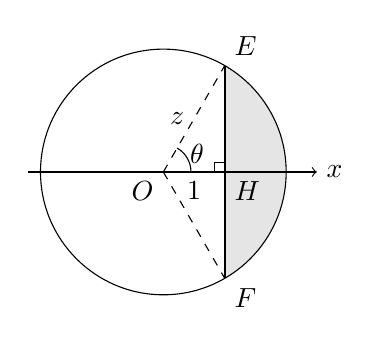
\begin{tikzpicture}[scale=0.78]
        \fill[gray!20] (1,{-sqrt(3)}) arc[start angle=-60,end angle=60,radius=2] -- cycle;
        \draw (0,0) circle[radius=2];
        \draw[thick] (1,{-sqrt(3)}) -- (1,{sqrt(3)});
        \draw[dashed] (0,0) -- (1,{sqrt(3)}) node[midway,left] {$z$};
        \draw[dashed] (0,0) -- (1,{-sqrt(3)});
        \draw[->] (-2.2,0) -- (2.5,0) node[right] {$x$};
        \draw (0.45,0) arc[start angle=0,end angle=60,radius=0.45];
        \node at (0.55,0.30) {$\theta$};
        \node[below left] at (0,0) {$O$};
        \node[below right] at (1,0) {$H$};
        \node[above right] at (1,{sqrt(3)}) {$E$};
        \node[below right] at (1,{-sqrt(3)}) {$F$};
        \node[below] at (0.5,0) {$1$};
        \draw (0.84,0) -- (0.84,0.16) -- (1,0.16);
      \end{tikzpicture}
      \BookFigureCaption{立体の水平断面と円弧・弦}
    \end{center}
    その面積を$A(z)$とすると,扇形から三角形を引いて,
    \[
      \begin{aligned}
        A(z)&=\frac12z^2\cdot2\theta
        -\frac12\cdot2\sqrt{z^2-1}\cdot1\\
        &=z^2\theta-\sqrt{z^2-1}.
      \end{aligned}
    \]
    よって体積は$V=\int_1^2 A(z)\,dz$である.
    $\displaystyle z=\frac{1}{\cos\theta}$と置けば,
    \[
      \sqrt{z^2-1}=\tan\theta,
      \qquad dz=\frac{\sin\theta}{\cos^2\theta}\,d\theta.
    \]
    したがって,
    \[
      \begin{aligned}
        V&=\int_0^{\frac{\pi}{3}}\frac{\theta\sin\theta}{\cos^4\theta}\,d\theta\\
        &\quad-\int_0^{\frac{\pi}{3}}\frac{\sin^2\theta}{\cos^3\theta}\,d\theta.
      \end{aligned}
    \]
    第一項では$\displaystyle (\cos^{-3}\theta)'=\frac{3\sin\theta}{\cos^4\theta}$を使って部分積分する.
    第二項では$\sin^2\theta=1-\cos^2\theta$を使うと,
    \[
      \begin{aligned}
        V&=\left[\frac{\theta}{3\cos^3\theta}\right]_0^{\frac{\pi}{3}}
        -\frac13I_3-(I_3-I_1)\\
        &=\frac{8\pi}{9}-\frac43I_3+I_1\\
        &=\frac{8\pi}{9}-\frac{4\sqrt3}{3}
        +\frac13\log(2+\sqrt3).
      \end{aligned}
    \]
    断面の半径と切断位置の関係を角度で表すと,最初に調べた$I_3$が自然に現れた.
    積分の\bookterm{recurrence}{漸化式}は\bookterm{sequence}{数列}だけの技法ではなく,図形から生まれる積分を計算するためにも使える.
    % F6: 一般項を求めずに減衰の速さを決める
  \item 分母に$a_n$があるが,本編の分数型と違って分母が二乗になっている.
    まず逆数を取って,\bookterm{general}{一般項}が求められるかだけでなく,増え方を評価できるかを調べる.
    \par\noindent
    \textbf{(1) 逆数の\bookterm{difference}{階差}を足す.}
    $a_1=1>0$であり,$a_n>0$なら$(1+2a_n)^2>0$なので$a_{n+1}>0$である.
    よって\bookterm{induction}{数学的帰納法}からすべての項が正で,$\displaystyle b_n=\frac{1}{a_n}$も定義できる.
    逆数を取ると,
    \[
      \begin{aligned}
        b_{n+1}&=\frac{(1+2a_n)^2}{a_n}\\
        &=b_n+4+4a_n.
      \end{aligned}
    \]
    したがって$b_{n+1}-b_n=4+4a_n>4$である.
    $k=1,\ldots,n-1$について足すと,
    \[
      b_n-b_1=4(n-1)+4\sum_{k=1}^{n-1}a_k.
    \]
    $b_1=1$より,
    \[
      b_n=4n-3+4\sum_{k=1}^{n-1}a_k.
    \]
    $n\geq2$なら右辺の総和は正だから,$b_n>4n-3$となる.
    ここまでの変形は,逆数化したあとに\bookterm{difference}{階差}を総和する本編の技法である.
    ただし総和に$a_k$が残っているため,この式だけでは\bookterm{general}{一般項}は得られていない.
    \par\noindent
    \textbf{(2) 項の収束と平均.}
    正の数の逆数を取ると不等号が逆向きになるので,
    \[
      0<a_n<\frac1{4n-3}\qquad(n\geq2).
    \]
    挟み撃ちの原理より$a_n\to0$である.
    しかし平均にも$n$が入っているので,項の\bookterm{limit}{極限}だけで終えず,平均を直接評価する.
    任意の正数$\varepsilon$を取る.
    $a_n\to0$より,$k\geq N$なら$0<a_k<\varepsilon$となる正整数$N$が存在する.
    $C=\sum_{k=1}^{N-1}a_k$と置けば,$C$は$n$によらない定数である.
    $n\geq N$のとき,
    \[
      \begin{aligned}
        0<\frac1n\sum_{k=1}^{n}a_k
        &=\frac Cn+\frac1n\sum_{k=N}^{n}a_k\\
        &\leq\frac Cn+\frac{n-N+1}{n}\varepsilon\\
        &\leq\frac Cn+\varepsilon.
      \end{aligned}
    \]
    十分大きい$n$では$\displaystyle \frac{C}{n}<\varepsilon$でもあるため,平均は$2\varepsilon$より小さい.
    $\varepsilon$はいくらでも小さく取れるので,
    \[
      \lim_{n\to\infty}\frac1n\sum_{k=1}^{n}a_k=0.
    \]
    この証明では,大きかった最初の有限個の項の影響は$n$で割ると消え,
    残りの項はすべて小さい,という二つの点を使っている.
    \par\noindent
    \textbf{(3) 逆数から減り方を読む.}
    (1)の等式を$n$で割ると,
    \[
      \frac{b_n}{n}=4-\frac3n+
      \frac4n\sum_{k=1}^{n-1}a_k.
    \]
    (2)より,
    \[
      0\leq\frac1n\sum_{k=1}^{n-1}a_k
      \leq\frac1n\sum_{k=1}^{n}a_k\longrightarrow0.
    \]
    したがって$\displaystyle \frac{b_n}{n}\to4$であり,
    \[
      na_n=\cfrac{1}{\frac{b_n}{n}}\longrightarrow\frac14.
    \]
    \par
    最初に求めた上界は,$a_n\to0$を示すための中間結果である.
    それによって\bookterm{difference}{階差}の追加項$4a_n$の平均が消え,$b_n$は最終的に$4n$と同じ割合で増えると分かった.
    結論$\displaystyle na_n\to\frac{1}{4}$は,$a_n$の減少の速さが$\displaystyle \frac{1}{4n}$のそれに近づくことを表す.
    このように,\bookterm{general}{一般項}を閉じた式で表さなくても,\bookterm{recurrence}{漸化式}から\bookterm{sequence}{数列}の主要な性質を決められる.
    % F7: 1往復で整列できる札の配置
  \item \textbf{(1)~小さい例と左端の札.}
    二枚ならすべて成功して$c_2=2$となる.
    三枚では往路で$3$が右端へ移り,復路の最後に残り二枚が昇順になるので$c_3=6$である.
    一般に最初の比較後,左端には$b=\min(A_1,A_2)$が残る.
    その後でこの札に触れるのは復路の最後だけだから,最終位置は左から一番目か二番目である.
    成功配置では$b\le2$が必要だが,これだけでは十分でない.
    \smallskip\textbf{(2)~札を戻せる対応.}
    数字を小さい順に読み替えても,比較・交換の動きは変わらない.
    (1)により成功配置を次の四種類に分ける.
    \[
      \begin{array}{ll}
        \text{\textcircled{1}}&A_1=1,\\
        \text{\textcircled{2}}&A_2=1,\\
        \text{\textcircled{3}}&A_1=2,\ A_2\ge3,\\
        \text{\textcircled{4}}&A_2=2,\ A_1\ge3.
      \end{array}
    \]
    \textbf{\textcircled{1},\textcircled{2}の数え方.}
    最初の比較後に左端にある$1$を除くと,残る$n-1$枚への操作は小さい問題と同じになる.
    復路の最後の$1$との比較は交換を起こさないので,成否も一致する.
    逆に数字をすべて$1$増やし,$1$を先頭または二番目へ挿入すれば一意に戻せる.
    よって各種類は$c_{n-1}$通りである.
    \par\textbf{\textcircled{3}の数え方.}
    先頭の$2$を除き,$1$はそのまま,$3,\ldots,n$を$2,\ldots,n-1$に読み替える.
    縮約先の先頭は$1$でない.
    例えば$(2,4,3,1)$は$(3,2,1)$に対応し,操作は次のようになる.
    \[
      \begin{array}{c|c|c}
        &\text{元の配置}&\text{縮約配置}\\ \hline
        \text{開始}&(2,4,3,1)&(3,2,1)\\
        \text{往路後}&(2,3,1,4)&(2,1,3)\\
        \text{復路後}&(1,2,3,4)&(1,2,3)
      \end{array}
    \]
    \BookMathLayout{一般にも往路後の元の配列は$(2,B_1,\ldots,B_{n-1})$で,後ろの札への操作は縮約問題と同じである.}{一般にも往路後の元の配列は\newline
      $(2,B_1,\ldots,B_{n-1})$で,後ろの札への操作は縮約問題と同じである.}
    復路では最小の札$1$がその部分の左端へ移るため,最後の比較直前には
    $(2,1,D_2,\ldots,D_{n-1})$となる.
    最後の$(2,1)$を交換すれば,元の成否と縮約先の成否が一致する.
    逆に,先頭が$1$でない成功配置で数字$2$以上を$1$増やし,先頭に$2$を戻せば一意に復元できる.
    先頭が$1$の成功配置は\textcircled{1}の対応から$c_{n-2}$通りなので,
    \textcircled{3}は$c_{n-1}-c_{n-2}$通りとなる.
    \par\textbf{\textcircled{4}の数え方.}
    最初の二枚を交換すれば\textcircled{3}に一対一で対応し,最初の比較後は同じ配列になる.
    よってこちらも$c_{n-1}-c_{n-2}$通りであり,
    \[
      c_n=2c_{n-1}+2(c_{n-1}-c_{n-2})
      =4c_{n-1}-2c_{n-2}.
    \]
    引いた$c_{n-2}$は,\textcircled{3}の縮約先から除く「先頭が$1$の配置」の数である.
    \smallskip\textbf{(3)~個数から3項型へ.}
    \bookterm{characteristic}{特性方程式}$x^2-4x+2=0$の根は$2\pm\sqrt2$である.
    \[
      c_n=P(2+\sqrt2)^{n-1}+Q(2-\sqrt2)^{n-1}
    \]
    に$c_1=1,c_2=2$を入れると$P=Q=\dfrac{1}{2}$であり,解答の式を得る.
    $c_4=20,c_5=68$となる.二つのべきで$\sqrt2$の奇数次の項が相殺され,個数は整数になる.
    この問の中心は,解く前の「何を取り除き,どう戻すか」という設計にある.
    % F8: 巨大な項の整除と, 添字の互除法
  \item \textbf{(1)~余りの\bookterm{recurrence}{漸化式}.}\par\nobreak
    項は$1,2,5,26,677,\ldots$と急増するが,法$5$で余りの更新を追えば,
    \[
      1\longmapsto2\longmapsto0\longmapsto1
    \]
    と繰り返す.同じ余りから次は一意に決まるため,$5$の倍数となるのは$n=3,6,9,\ldots$である.
    \smallskip\textbf{(2)~項を法に取る.}
    $a_0=0$を補えば更新は$n\ge0$で使える.正整数$m$を固定すると,
    \[
      a_{m+j}\equiv a_j\pmod{a_m}\quad(j\ge0)
    \]
    が成り立つ.$j=0$では両辺が零であり,次も$a_{m+j}^2+1\equiv a_j^2+1$なので,
    \bookterm{induction}{数学的帰納法}で示せる.
    $n=qm+r$（$0\le r<m$）としてこの合同式を繰り返すと,
    $a_n\equiv a_r\pmod{a_m}$となる.
    また$a_{n+1}-a_n=a_n(a_n-1)+1>0$より$a_0$から厳密に増加するので,
    $0\le a_r<a_m$かつ$a_r=0$は$r=0$の場合だけである.
    よって,
    \[
      \begin{aligned}
        a_m\mid a_n&\ \Longleftrightarrow\ a_r=0\\
        &\ \Longleftrightarrow\ r=0\ \Longleftrightarrow\ m\mid n.
      \end{aligned}
    \]
    $m=1$でも$r=0$なので成り立つ.(1)は$a_3=5$を用いた$m=3$の場合に当たる.
    \smallskip\textbf{(3)~項から添字の互除法へ.}
    $a_n-a_r$は$a_m$の倍数なので,共通の約数は変わらず,
    \[
      \gcd(a_m,a_n)=\gcd(a_m,a_r).
    \]
    \BookMathLayout{添字の互除法に沿って進むと,$d=\gcd(m,n)$と$0$で終わるため,}{添字の互除法に沿って進むと,\newline
      $d=\gcd(m,n)$と$0$で終わるため,}
    \[
      \gcd(a_m,a_n)=\gcd(a_d,a_0)=a_d.
    \]
    最後は$a_0=0$と$\gcd(x,0)=x$を使った.
    例では$3040=2026+1014$, $2026=1014+1012$, $1014=1012+2$, $1012=506\cdot2$より$d=2$である.
    したがって$\gcd(a_{2026},a_{3040})=a_2=2$となる.
    巨大な項どうしの整除関係を,小さな添字の計算へ移せた.
    % F9: 整数方程式の解を生み出す漸化式
  \item \textbf{(1)~一つの解から次の解へ.}
    $9+y^2+z^2=3yz$を$y$の二次方程式と見ると,もう一つの根は$3z-y$である.
    実際,
    \[
      \begin{aligned}
        &9+z^2+(3z-y)^2-3z(3z-y)\\
        &\qquad=9+y^2+z^2-3yz=0.
      \end{aligned}
    \]
    $3z-y$は整数で,$0<y\le z$より$3z-y\ge2z>z>0$となる.
    新しい二項も大小関係を満たすため,操作を繰り返せる.
    \smallskip\textbf{(2)~整数解を\bookterm{sequence}{数列}にする.}
    $(3,3,3)$からの操作で,$y,z$は$(3,3),(3,6),(6,15),(15,39),\ldots$と変わる.
    隣接する値を$u_n,u_{n+1}$とすれば$u_{n+2}=3u_{n+1}-u_n$となる.
    \bookterm{characteristic}{特性方程式}$t^2-3t+1=0$の根を$\alpha,\beta$とし,
    $u_n=P\alpha^n+Q\beta^n$とおく.
    $u_0=u_1=3$から,
    \[
      P=\frac{3(\sqrt5-1)}{2\sqrt5},\quad
      Q=\frac{3(\sqrt5+1)}{2\sqrt5}
    \]
    となり,解答の式を得る.
    \smallskip\textbf{(3)~整数性と方程式の確認.}
    初期値と更新の係数から全項が整数である.
    $u_2=6>u_1=3$であり,$u_{n+1}>u_n>0$なら$u_{n+2}>2u_{n+1}>u_{n+1}$となるため,
    $n\ge1$で正値と厳密な増加が続く.
    隣接する二項から作る
    \[
      I_n=u_n^2+u_{n+1}^2-3u_nu_{n+1}
    \]
    に更新式を入れると,
    \[
      \begin{aligned}
        I_{n+1}&=u_{n+1}^2+(3u_{n+1}-u_n)^2\\
        &\quad-3u_{n+1}(3u_{n+1}-u_n)=I_n.
      \end{aligned}
    \]
    よって$I_n=I_0=-9$から$(3,u_n,u_{n+1})$は正の整数解となる.
    増加するため解は互いに異なり,無限個得られる.ここでは全解の分類まではしていない.
    最後に$0<\beta<1<\alpha$と$P,Q>0$から,
    \[
      \frac{u_{n+1}}{u_n}
      =\alpha\,\cfrac{P+Q(\frac\beta\alpha)^{n+1}}
      {P+Q(\frac\beta\alpha)^n}
      \longrightarrow\alpha.
    \]
    更新式は整数性を保証し,\bookterm{general}{一般項}は整数の比が近づく無理数を示している.
    % F10: 元のペアをすべて解消する組み替え
  \item \textbf{(1) 小さい場合を数える.}
    $n=1$では相手がいないので$S(1)=0$である.
    $n=2$では$(A_1,B_2),(A_2,B_1)$の一通り,
    $n=3$では相手の添字が$(2,3,1),(3,1,2)$の二通りである.
    $S(0)=1$は「何も作らない組合せ」を一通りと数える約束である.
    \par\smallskip\textbf{(2) 相手を決めて分ける.}
    $A_1$の相手$B_j$を$j\ne1$の$n-1$通りから選び,固定する.
    $A_j$の相手が$B_1$なら,この二組の四要素を除く.
    残る添字は両側とも$1,j$以外であり,同じ添字のペアを禁止する条件も変わらない.
    したがって,残る$n-2$組の組み方は$S(n-2)$通りである.
    そうでない場合,$B_1$の相手を$A_k$（$k\ne1,j$）とする.
    この場合に四要素をそのまま除くと,両側で消える添字が異なり,残る問題の条件が変わってしまう.
    そこで,二組を一組につなぎ直す.
    \[
      (A_1,B_j),(A_k,B_1)\ \longmapsto\ (A_k,B_j)
    \]
    除くのは$A_1,B_1$だけで,$A_k,B_j$は残る.
    $k\ne j$なので新しいペアも元のペアではなく,ほかのペアは変わらない.
    これで,添字$2,\ldots,n$の元のペアを一組も含まない組み替えが得られる.
    \par
    逆に,この$n-1$組の組み替えを任意に取る.
    $B_j$の相手は一意に決まる$A_k$であり,元のペアがないので$k\ne j$である.
    $(A_k,B_j)$を$(A_1,B_j),(A_k,B_1)$に戻せば,元の配置を一意に復元できる.
    この一対一対応から,後者は$S(n-1)$通りである.
    ここで固定しているのは$j$であり,$k$の異なる場合はすべて$S(n-1)$に含まれている.
    $j$の選び方が$n-1$通りなので,
    \[
      S(n)=(n-1)\{S(n-1)+S(n-2)\}.
    \]
    \par\smallskip\textbf{(3) 差と階乗で整理する.}
    係数が$n$で変わるため,\bookterm{constant}{定数係数}の特性方程式は使えない.
    $T_n=S(n)-nS(n-1)$とおくと,$n\ge2$で,
    \[
      T_n=(n-1)S(n-2)-S(n-1)=-T_{n-1}.
    \]
    $T_1=-1$から$T_n=(-1)^n$となる.
    $S(n)=nS(n-1)+(-1)^n$の倍率を階乗へ吸収し,$P_n=\dfrac{S(n)}{n!}$とおけば,
    \[
      P_n-P_{n-1}=\frac{(-1)^n}{n!},\quad P_0=1.
    \]
    \bookterm{difference}{階差}を足すと,
    \[
      S(n)=n!\sum_{k=0}^n\frac{(-1)^k}{k!}.
    \]
    $S(4)=9,S(5)=44$となる.
    等比型,\bookterm{ratio}{階比}による\bookterm{normalize}{正規化},\bookterm{difference}{階差}型を順に使った.
    \par\smallskip\textbf{(4) 残る組数で数える.}
    残す$r$組を選び,残りを完全に組み替えれば$\binom nrS(n-r)$通りである.
    残るペアは完成形から一意に決まり,$r=n$も$S(0)=1$によって含む.
    平均には,固定した元のペアが残る$(n-1)!$通りを$n$組分数える.
    $r$組残る配置は$r$回数えられるので,残る組数の合計は$n(n-1)!$であり,平均は$\dfrac{n(n-1)!}{n!}=1$となる.
    \par\smallskip\noindent\textbf{【確率として読む】}\par\nopagebreak[4]
    元の位置に戻る要素のない並べ替えを\textbf{完全順列（錯置）}という.
    全$n!$通りが等確率なら,元のペアが一組も残らない確率は,
    \[
      P_n=\frac{S(n)}{n!}=\sum_{k=0}^n\frac{(-1)^k}{k!}.
    \]
    階乗で割る操作は,\textbf{個数を確率に直す操作}でもある.
    \par\smallskip\noindent\textbf{【偶奇に分けて極限を確かめる】}\par\nopagebreak[4]
    まず収束を示し,その後で値を決める.無限級数展開は仮定せず,
    \bookterm{binomial}{二項定理}と\sectionref*{節：対数}の$e$の定義を使う.
    \[
      \begin{aligned}
        P_{2m+2}-P_{2m}&=-\frac{2m+1}{(2m+2)!}<0,\\
        P_{2m+3}-P_{2m+1}&=\frac{2m+2}{(2m+3)!}>0,\\
        P_{2m}-P_{2m+1}&=\frac1{(2m+1)!}\longrightarrow0.
      \end{aligned}
    \]
    偶数番目は減少,奇数番目は増加し,確率は$0$以上$1$以下である.
    よって両者は共通の\bookterm{limit}{極限}$L$をもつ.
    \par\smallskip\noindent\textbf{【二項定理で極限の値を決める】}\par\nopagebreak[4]
    整数$M\ge2$について$b_{M,k}=\dfrac{\binom Mk}{M^k}$とおくと,
    \[
      \frac{b_{M,k+1}}{b_{M,k}}=\frac{M-k}{M(k+1)}\le1
      \quad(0\le k<M).
    \]
    有限の二項展開を途中で止め,残りを隣り合う二項ずつ組にする.
    奇数で止めた残りは非負,偶数で止めた残りは非正なので,$M\ge2\ell+1$では,
    \[
      \begin{aligned}
        \sum_{k=0}^{2\ell+1}(-1)^kb_{M,k}
        &\le\left(1-\frac1M\right)^M,\\
        \left(1-\frac1M\right)^M
        &\le\sum_{k=0}^{2\ell}(-1)^kb_{M,k}.
      \end{aligned}
    \]
    \textbf{まず$\ell$を固定して$M\to\infty$とする.}
    和の項数は固定され,各項で,
    \[
      b_{M,k}=\frac1{k!}\prod_{j=0}^{k-1}\left(1-\frac jM\right)
      \longrightarrow\frac1{k!}
    \]
    となる.$k=0$の空積は$1$である.
    一方,$t=M-1$とおくと,
    \[
      \left(1-\frac1M\right)^M=\left(1+\frac1t\right)^{-t-1}
      \longrightarrow\frac1e
    \]
    である.$\left(1+\dfrac{1}{t}\right)^t\to e$と$1+\dfrac{1}{t}\to1$を使った.
    したがって$P_{2\ell+1}\le\dfrac{1}{e}\le P_{2\ell}$となる.
    \textbf{次に$\ell\to\infty$とする.}両端が$L$へ近づくため,
    \[
      \boxed{\lim_{n\to\infty}\frac{S(n)}{n!}=\frac1e\simeq0.368}.
    \]
    \par\smallskip\noindent\textbf{【個数はどこまで近いか】}\par\nopagebreak[4]
    偶奇の各列が厳密に進むので,$\dfrac{1}{e}$は隣り合う$P_n,P_{n+1}$の間に厳密に入る.
    よって$n\ge1$で,
    \[
      \begin{aligned}
        \left|P_n-\frac1e\right|&<\frac1{(n+1)!},\\
        \left|S(n)-\frac{n!}e\right|&<\frac1{n+1}\le\frac12.
      \end{aligned}
    \]
    下段は上段を$n!$倍したものであり,$S(n)$は$\dfrac{n!}{e}$に最も近い整数となる.
    数え上げの\bookterm{recurrence}{漸化式}が,階乗・確率・自然\bookterm{logarithm}{対数}の底を結んだ.
\end{enumerate}

% BOOK-FILE-ID: f-49d89f9a5544
\subsection{発展・特殊型}\label{節：発展・特殊型}
\sectionref{節：発展的な解法}と\sectionref{節：式の構造を使う}の15題である.
\bookterm{floor}{ガウス記号}には整数性・余り,多項間の関係には\bookterm{difference}{階差}・\bookterm{characteristic}{特性方程式},
\bookterm{nonlinear}{非線形}な式には対称式・\bookterm{trigonometric}{三角関数}の恒等式を使う.
候補は\bookterm{initial}{初期条件}と漸化式で確かめ,分母や角度の定義域も確認する.
問14・問15では初項を動かし,定\bookterm{sequence}{数列}・周期列・有界な\bookterm{sequence}{数列}が現れる条件を調べる.有界や$+\infty$への発散の意味は\sectionref*{節：数列の極限}を参照する.
以下,特に指定しない限り,$n$は正の整数とする.
$\lfloor x\rfloor$は$x$を超えない最大の整数を表す.
周期の最小値とは,すべての添字で$a_{n+p}=a_n$となる正の整数$p$の最小値をいう.

\subsubsection{問題}\label{節：発展・特殊型：問題}
\begin{enumerate}[label=\textbf{問\arabic*.},leftmargin=3.8em,format=\bookitemlink{practice-special}{problem}{answer}]
  % E1: ガウス型・整数の半減
  \item \bookterm{sequence}{数列}$\{a_n\}$を
    \[
      a_1=2026,\qquad
      a_{n+1}=\left\lfloor\frac{a_n}{2}\right\rfloor
    \]
    によって定める.
    \par\smallskip\noindent
    (1) \bookterm{general}{一般項}を求めよ.
    \par\smallskip\noindent
    (2) 初めて$a_n=0$となる添字$n$を求めよ.
    \par\smallskip\noindent
    (3) 非負整数$M$に対し,別の数列を
    \[
      b_1=M,\qquad
      b_{n+1}=\left\lfloor\frac{b_n+6}{2}\right\rfloor
    \]
    と定める.$b_n$の一般項と,最終的に一定になる値を求めよ.
    % E2: ガウス型・三つずつの群
  \item \bookterm{sequence}{数列}$\{a_n\}$を
    \[
      a_0=0,\qquad
      a_{n+1}=a_n+\left\lfloor\frac{n+1}{3}\right\rfloor
      \quad(n\ge0)
    \]
    によって定める.\,
    (1) $n=3q+r$（$q\ge0$,$r=0,1,2$）とおき,
    \bookterm{general}{一般項}を$q,r$で表せ.
    \par\smallskip\noindent
    (2) $a_n$を,次の範囲にある格子点（座標がともに整数の点）の個数として説明せよ.
    \[
      1\le x\le n,\qquad 1\le y\le\frac{x}{3}.
    \]
    % E3: ガウス型・余りの有限個の状態
  \item \bookterm{sequence}{数列}$\{a_n\}$を
    \[
      a_1=1,\qquad
      a_{n+1}=2a_n+1
      -5\left\lfloor\frac{2a_n+1}{5}\right\rfloor
    \]
    によって定める.
    \par\smallskip\noindent
    (1) すべての項が$0,1,2,3,4$のいずれかになることを示せ.
    \par\smallskip\noindent
    (2) \bookterm{general}{一般項}を,$n$を$4$で割った余りで場合分けして表せ.
    また,周期の最小値を求めよ.
    % E4: 隣接4項間・三階差が定数
  \item \bookterm{sequence}{数列}$\{a_n\}$を
    \[
      a_1=2,\qquad a_2=9,\qquad a_3=28,
    \]
    \[
      a_{n+3}=3a_{n+2}-3a_{n+1}+a_n+6
    \]
    によって定める.
    \par\smallskip\noindent
    (1) $d_n=a_{n+2}-2a_{n+1}+a_n$とおき,$d_n$を求めよ.
    \par\smallskip\noindent
    (2) \bookterm{general}{一般項}を求めよ.
    % E5: 隣接4項間・異なる三つの特性根
  \item \bookterm{sequence}{数列}$\{a_n\}$を
    \[
      a_1=3,\qquad a_2=6,\qquad a_3=14,
    \]
    \[
      a_{n+3}=6a_{n+2}-11a_{n+1}+6a_n
    \]
    によって定める.
    \par\smallskip\noindent
    (1) $d_n=a_{n+2}-3a_{n+1}+2a_n$とおき,$d_n$を求めよ.
    \par\smallskip\noindent
    (2) \bookterm{general}{一般項}を求めよ.
    % E6: 虚数解型・周期6
  \item \bookterm{sequence}{数列}$\{a_n\}$を
    \[
      a_1=0,\qquad a_2=1,\qquad
      a_{n+2}=a_{n+1}-a_n
    \]
    によって定める.
    \par\smallskip\noindent
    (1) \bookterm{trigonometric}{三角関数}を用いて\bookterm{general}{一般項}を表せ.
    \par\smallskip\noindent
    (2) 周期の最小値を求めよ.
    % E7: 虚数解型・振幅が減衰する数列
  \item \bookterm{sequence}{数列}$\{a_n\}$を
    \[
      a_1=1,\qquad a_2=0,\qquad
      a_{n+2}=a_{n+1}-\frac12a_n
    \]
    によって定める.\bookterm{trigonometric}{三角関数}を用いて\bookterm{general}{一般項}を表し,
    $\lim_{n\to\infty}a_n$を求めよ.
    % E8: 非隣接2項間・奇数列と偶数列の逆数
  \item \bookterm{sequence}{数列}$\{a_n\}$を
    \[
      a_1=1,\qquad a_2=2,\qquad
      a_{n+2}=\frac{a_n}{1+a_n}
    \]
    によって定める.
    \par\smallskip\noindent
    (1) すべての項が正であることを示し,
    $a_{2k-1},a_{2k}$を$k$で表せ.
    ただし,$k$は正の整数とする.
    \par\smallskip\noindent
    (2) $\lim_{n\to\infty}a_n$を求めよ.
    % E9: 基本対称式型・平行移動して恒等式を使う
  \item \bookterm{sequence}{数列}$\{a_n\}$を
    \[
      a_1=\frac72,\qquad
      a_{n+1}=a_n^2-2a_n
    \]
    によって定める.
    \par\smallskip\noindent
    (1) $b_n=a_n-1$とおき,$b_n$の\bookterm{recurrence}{漸化式}を求めよ.
    \par\smallskip\noindent
    (2) 恒等式
    \[
      \left(u+u^{-1}\right)^2-2=u^2+u^{-2}
      \quad(u\ne0)
    \]
    を用いて$a_n$の\bookterm{general}{一般項}を求めよ.
    % E10: 基本対称式型・三乗の対称式
  \item \bookterm{sequence}{数列}$\{a_n\}$を
    \[
      a_1=\frac52,\qquad
      a_{n+1}=a_n^3-3a_n
    \]
    によって定める.
    \par\smallskip\noindent
    (1) 恒等式
    \[
      \left(u+u^{-1}\right)^3
      -3\left(u+u^{-1}\right)=u^3+u^{-3}
    \]
    を示せ.ただし,$u\ne0$とする.
    \par\smallskip\noindent
    (2) \bookterm{general}{一般項}を求めよ.
    % E11: 三角関数型・余弦の倍角と周期3
  \item \bookterm{sequence}{数列}$\{a_n\}$を
    \[
      a_1=\cos\frac{2\pi}{7},\qquad
      a_{n+1}=2a_n^2-1
    \]
    によって定める.
    \par\smallskip\noindent
    (1) \bookterm{general}{一般項}を求めよ.
    \par\smallskip\noindent
    (2) 周期の最小値を求めよ.
    % E12: 三角関数型・正接の定義域と周期4
  \item 初項と次の項を計算する規則を
    \[
      a_1=\tan\frac{\pi}{5},\qquad
      a_{n+1}=\frac{2a_n}{1-a_n^2}
    \]
    とする.
    \par\smallskip\noindent
    (1) \bookterm{general}{一般項}の候補を求め,すべての段階で分母が$0$にならず,
    \bookterm{sequence}{数列}が定義できることを示せ.
    \par\smallskip\noindent
    (2) 周期の最小値を求めよ.
    % E13: ニュートン法型・初項が収束先より小さい場合
  \item \bookterm{sequence}{数列}$\{a_n\}$を
    \[
      a_1=1,\qquad
      a_{n+1}=\frac{a_n^2+3}{2a_n}
    \]
    によって定める.
    \par\smallskip\noindent
    (1) すべての項が正であることを示せ.
    \par\smallskip\noindent
    (2) $b_n=\frac{a_n-\sqrt3}{a_n+\sqrt3}$とおき,
    $b_n,a_n$の\bookterm{general}{一般項}を求めよ.
    \par\smallskip\noindent
    (3) $n\ge2$で$a_n>\sqrt3$かつ
    $a_{n+1}<a_n$であることを示し,$\lim_{n\to\infty}a_n$を求めよ.
    % E14: 初項依存型・不動点と2周期点
  \item 実数$c$を初項として,\bookterm{sequence}{数列}$\{a_n\}$を
    \[
      a_1=c,\qquad a_{n+1}=a_n^2-1
    \]
    によって定める.
    \par\smallskip\noindent
    (1) \bookterm{sequence}{数列}が定\bookterm{sequence}{数列}となる$c$をすべて求めよ.
    \par\smallskip\noindent
    \BookMathLayout{(2) 定\bookterm{sequence}{数列}ではなく,すべての$n$で$a_{n+2}=a_n$を満たす
      $c$をすべて求め,それぞれの場合の\bookterm{general}{一般項}を表せ.}{(2) 定\bookterm{sequence}{数列}ではなく,\\すべての$n$で$a_{n+2}=a_n$を満たす
      $c$をすべて求め,それぞれの場合の\bookterm{general}{一般項}を表せ.}
    % E15: 初項依存型・有界になる初項の範囲
  \item 実数$c$を初項として,\bookterm{sequence}{数列}$\{a_n\}$を
    \[
      a_1=c,\qquad a_{n+1}=a_n^2-2
    \]
    によって定める.
    \par\smallskip\noindent
    (1) $c=-2,-1,0,2$のそれぞれについて,最初の4項を求めよ.
    \par\smallskip\noindent
    (2) $-2\le c\le2$のとき,$c=2\cos\theta$
    （$0\le\theta\le\pi$）とおき,\bookterm{general}{一般項}を求めよ.
    また,すべての項が$-2$以上$2$以下であることを示せ.
    \par\smallskip\noindent
    (3) $|c|>2$のとき,$a_n\to+\infty$を示せ.
    以上から,\bookterm{sequence}{数列}が有界となる$c$の範囲を求めよ.
\end{enumerate}

\subsubsection{方針}\label{節：発展・特殊型：方針}
\begin{enumerate}[label=\textbf{問\arabic*.},leftmargin=3.8em,format=\bookitemlink{practice-special}{hint}{problem}]
  % E1
  \item 整数を$2$で割った商と余りに分け,
    $\left\lfloor\frac{\lfloor x\rfloor}{2}\right\rfloor
      =\left\lfloor\frac{x}{2}\right\rfloor$となることを確かめる.
    初めて$0$になる位置は,$2026$と$2$の累乗を比べればよい.
    (3)では$b_n-6$を考え,負の数の切り捨てにも注意する.
    % E2
  \item \bookterm{difference}{階差}を足すと$\sum_{k=1}^{n}\lfloor\frac{k}{3}\rfloor$になる.
    同じ値を取る添字を三つずつまとめ,最後の群を$r+1$項として数える.
    $\lfloor\frac{k}{3}\rfloor$は,$x=k$上にある指定範囲の格子点の個数でもある.
    % E3
  \item $x-5\lfloor\frac{x}{5}\rfloor$は整数$x$を$5$で割った余りである.
    項の値が五つに絞れたら,それぞれが次にどの値へ移るかを表にする.
    % E4
  \item $d_{n+1}-d_n$を作ると元の\bookterm{recurrence}{漸化式}を移項した式の左辺が現れる.
    その後,$e_n=a_{n+1}-a_n$を求め,もう一度足して$a_n$へ戻す.
    % E5
  \item $d_{n+1}-3d_n$を展開すると$0$になる.
    得られた3項間の式を満たす$3^{n-1}$を引き,残りを解く.
    % E6
  \item \bookterm{characteristic}{特性方程式}の根の絶対値と\bookterm{argument}{偏角}を調べる.
    最初の二つの項に合う$\sin$の式を作り,実際の値の並びから周期を確かめる.
    % E7
  \item 特性方程式の解の絶対値は$1$未満である.
    \bookterm{polar}{極形式}から\bookterm{trigonometric}{三角関数}の\bookterm{general}{一般項}を作り,その絶対値を\bookterm{geometric}{等比数列}で上から押さえる.
    % E8
  \item 正値を確かめてから逆数を取る.
    奇数番目と偶数番目を別々の\bookterm{sequence}{数列}にすると,二つの\bookterm{arithmetic}{等差数列}が得られる.
    % E9
  \item $a_n^2-2a_n=(a_n-1)^2-1$と\bookterm{square}{平方完成}する.
    $b_1=2+2^{-1}$と書けば,恒等式によって指数が毎回2倍になる.
    % E10
  \item 展開すると,交差項が$3(u+u^{-1})$であることが分かる.
    初項を$2+2^{-1}$と表し,指数を毎回3倍にする候補を作る.
    % E11
  \item 余弦の倍角公式で,角度を毎回2倍にする候補を作る.
    3回倍にした角度と元の角度との差が$2\pi$の整数倍になることを調べる.
    % E12
  \item 正接の倍角公式を使う.
    候補の角度が$\frac{\pi}{2}$に$\pi$の整数倍を加えた値になるかを,
    整数の偶奇で判断する.次の角度でも正接が定義できれば,\bookterm{recurrence}{漸化式}の分母も$0$にならない.
    % E13
  \item $a_{n+1}\pm\sqrt3$の分子は平方になる.比を取って$b_{n+1}=b_n^2$を導く.
    $b_1<0$なので,\bookterm{logarithm}{対数}を取らずにべき乗の形を帰納法で確かめる.
    減少を示す範囲が$n\ge2$であることにも注意する.
    % E14
  \item 定\bookterm{sequence}{数列}には$a_2=a_1$,周期2の候補には$a_3=a_1$が必要である.
    後者の方程式を因数分解し,定\bookterm{sequence}{数列}の初項を除く.残った初項が実際に二つの値を往復することも確かめる.
    % E15
  \item $|c|\le2$では$2\cos\theta$という表示を使う.
    $|c|>2$では第2項が$2$を超えるので,
    $a_{n+1}-2=(a_n-2)(a_n+2)$から下からの評価を作る.
\end{enumerate}

\subsubsection{答え}\label{節：発展・特殊型：答え}
\begin{enumerate}[label=\textbf{問\arabic*.},leftmargin=3.8em,format=\bookitemlink{practice-special}{answer}{problem}]
  % E1
  \item (1)
    \[
      a_n=\left\lfloor\frac{2026}{2^{n-1}}\right\rfloor.
    \]
    (2) $n=12$である.
    \par\smallskip\noindent
    (3)
    \[
      b_n=6+\left\lfloor\frac{M-6}{2^{n-1}}\right\rfloor.
    \]
    有限回の操作の後で,$M<6$なら$5$,$M\ge6$なら$6$に固定される.
    % E2
  \item (1)
    \[
      a_n=\frac{3q(q-1)}2+q(r+1),
    \]
    \[
      n=3q+r,\qquad q\ge0,\quad r=0,1,2.
    \]
    (2) $x=k$ごとに$\lfloor\frac{k}{3}\rfloor$個の点があり,その和が$a_n$である.
    % E3
  \item (1) 整数性と\bookterm{floor}{ガウス記号}の定義から,各項は$0$以上$4$以下の整数となる.
    \par\smallskip\noindent
    (2) $k$を$0$以上の整数として,
    \[
      a_{4k+1}=1,\quad a_{4k+2}=3,
    \]
    \[
      a_{4k+3}=2,\quad a_{4k+4}=0.
    \]
    周期の最小値は$4$である.
    % E4
  \item (1) $d_n=6n+6$.
    \par\smallskip\noindent
    (2) $a_n=n^3+1$.
    % E5
  \item (1) $d_n=2\cdot3^{n-1}$.
    \par\smallskip\noindent
    (2)
    \[
      a_n=1+2^{n-1}+3^{n-1}.
    \]
    % E6
  \item (1)
    \[
      a_n=\frac2{\sqrt3}\sin\frac{(n-1)\pi}{3}.
    \]
    (2) 周期の最小値は$6$である.
    % E7
  \item
    \[
      a_n=\left(\frac1{\sqrt2}\right)^{n-1}
      \left(\cos t_n-\sin t_n\right),
    \]
    \[
      t_n=\frac{(n-1)\pi}{4},\qquad
      \lim_{n\to\infty}a_n=0.
    \]
    % E8
  \item (1) すべての項は正であり,
    \[
      a_{2k-1}=\frac1k,\qquad
      a_{2k}=\frac2{2k-1}\quad(k\ge1).
    \]
    (2) \bookterm{limit}{極限}は$0$である.
    % E9
  \item (1) $b_1=\frac52$,$b_{n+1}=b_n^2-2$.
    \par\smallskip\noindent
    (2)
    \[
      a_n=1+2^{\,2^{n-1}}+2^{-2^{n-1}}.
    \]
    % E10
  \item (1) 左辺を展開すると右辺を得る.
    \par\smallskip\noindent
    (2)
    \[
      a_n=2^{\,3^{n-1}}+2^{-3^{n-1}}.
    \]
    % E11
  \item (1)
    \[
      a_n=\cos\left(2^{n-1}\frac{2\pi}{7}\right).
    \]
    (2) 周期の最小値は$3$である.
    % E12
  \item (1)
    \[
      a_n=\tan\left(2^{n-1}\frac{\pi}{5}\right).
    \]
    すべての項で正接が定義でき,\bookterm{recurrence}{漸化式}の分母も$0$にならない.
    \par\smallskip\noindent
    (2) 周期の最小値は$4$である.
    % E13
  \item (1) 初項が正で,正の項から次の正の項が定まる.
    \par\smallskip\noindent
    (2) $q=\sqrt3-2$とおくと,
    \[
      b_n=q^{\,2^{n-1}},\qquad
      a_n=\sqrt3\,\frac{1+q^{\,2^{n-1}}}{1-q^{\,2^{n-1}}}.
    \]
    (3) $n\ge2$で設問の二つの不等式が成り立ち,
    \[
      \lim_{n\to\infty}a_n=\sqrt3.
    \]
    % E14
  \item (1)
    \[
      c=\frac{1+\sqrt5}{2},\quad
      \frac{1-\sqrt5}{2}.
    \]
    それぞれ$a_n=c$である.
    \par\smallskip\noindent
    (2) $c=0,-1$であり,どちらも
    \[
      a_n=-\frac12+\left(c+\frac12\right)(-1)^{n-1}
    \]
    と表せる.周期の最小値は$2$である.
    % E15
  \item (1)
    \[
      \begin{array}{c|rrrr}
        c&a_1&a_2&a_3&a_4\\ \hline
        -2&-2&2&2&2\\
        -1&-1&-1&-1&-1\\
        0&0&-2&2&2\\
        2&2&2&2&2
      \end{array}
    \]
    (2)
    \[
      a_n=2\cos(2^{n-1}\theta),\qquad -2\le a_n\le2.
    \]
    (3) $n\ge2$で
    \[
      a_n\ge2+4^{n-2}(c^2-4)
    \]
    となり,$a_n\to+\infty$である.
    有界となる範囲は$-2\le c\le2$である.
\end{enumerate}

\subsubsection{解説}\label{節：発展・特殊型：解説}
\begin{enumerate}[label=\textbf{問\arabic*.},leftmargin=3.8em,format=\bookitemlink{practice-special}{solution}{problem}]
  % E1
  \item \textbf{(1)~整数部分を分ける.}
    \sectionref{節：ガウス記号を含む式}の整数性に着目する.
    実数$x$について,整数$\lfloor x\rfloor$を
    \[
      \lfloor x\rfloor=2q+r,\qquad r=0,1
    \]
    と表す.\bookterm{floor}{ガウス記号}の定義を使って$2$で割れば,
    \begin{align*}
      \frac x2&\ge q+\frac r2\ge q,\\
      \frac x2&<q+\frac{r+1}{2}\le q+1.
    \end{align*}
    したがって,
    \[
      \left\lfloor\frac{x}{2}\right\rfloor=q
      =\left\lfloor\frac{\lfloor x\rfloor}{2}\right\rfloor.
    \]
    $a_1=\lfloor2026\rfloor$であり,この恒等式を繰り返し使うと,
    \[
      a_n=\left\lfloor\frac{2026}{2^{n-1}}\right\rfloor
    \]
    が帰納法で得られる.

    \smallskip
    \textbf{(2)~1未満になる位置.}
    $2^{10}=1024\le2026<2048=2^{11}$だから,
    \[
      a_{11}=1,\qquad a_{12}=0.
    \]
    $n\le11$では切り捨てる前の値が$1$以上なので,
    初めて$0$となるのは$n=12$である.
    毎回の切り捨てを一つの\bookterm{floor}{ガウス記号}にまとめられる理由は,割る数が正の整数であることにある.

    \smallskip
    \textbf{(3)~整数を引いて同じ操作にする.}
    $c_n=b_n-6$とおく.整数をガウス記号の外へ出すと,
    \[
      c_{n+1}=\left\lfloor\frac{c_n}{2}\right\rfloor,
      \qquad c_1=M-6.
    \]
    (1)の恒等式は負の$x$にも成り立つので,
    \[
      c_n=\left\lfloor\frac{M-6}{2^{n-1}}\right\rfloor
    \]
    となる.十分大きな$n$では,中身が$M\ge6$なら$[0,1)$,$M<6$なら$(-1,0)$に入る.
    したがって$b_n$は,それぞれ$6$,$5$に有限回で到達する.
    実際,整数$x$が不動点となる条件は
    \[
      x\le\frac{x+6}{2}<x+1
      \iff 4<x\le6
    \]
    である.丸めを外した実数の漸化式の不動点は$6$だけだが,切り捨てると$5$も不動点となる.
    % E2
  \item \textbf{(1)~同じ値をまとめて足す.}
    \sectionref{節：同じ値を群にまとめる}の考え方を使う.
    \bookterm{difference}{階差}を足すと,
    \[
      a_n=\sum_{k=1}^{n}\left\lfloor\frac{k}{3}\right\rfloor.
    \]
    $k=1,2$では0で,$k=3j,3j+1,3j+2$では値が$j$になる.
    $n=3q+r$, $q\ge1$なら,値$1,\ldots,q-1$の群は三項ずつ,最後の値$q$の群は$r+1$項ある.
    よって,
    \begin{align*}
      a_n&=3\sum_{j=1}^{q-1}j+q(r+1)\\
      &=\frac{3q(q-1)}2+q(r+1).
    \end{align*}
    $q=0$でも実際の値と式は0である.
    最後の群は途中までなので,常に三項と数えてはいけない.

    \smallskip
    \textbf{(2)~和を個数として読む.}
    $x=k$のとき,指定範囲の整数$y$は$1$から$\lfloor\frac{k}{3}\rfloor$まである.
    $k=1,\ldots,n$について足せば,(1)の和に一致する.
    群ごとに値と項数を掛けて足す方法と,格子点の個数を数える方法は,同じ和の二つの見方である.
    % E3
  \item \textbf{(1)~余りに読み替える.}
    \sectionref{節：ガウス記号を含む式}では,\bookterm{floor}{ガウス記号}が整数問題の道具にもなる.
    整数$x$について\bookterm{floor}{ガウス記号}の定義から,
    \[
      0\le x-5\left\lfloor\frac{x}{5}\right\rfloor<5.
    \]
    整数なので値は$0,1,2,3,4$に限られる.
    初項の整数性と$x=2a_n+1$を使えば,帰納的に全項がこの範囲に入る.

    \smallskip
    \textbf{(2)~5つの値の移り方.}
    (1)より,次の表だけを調べれば十分である.
    \[
      \begin{array}{c|rrrrr}
        a_n&0&1&2&3&4\\ \hline
        a_{n+1}&1&3&0&2&4
      \end{array}
    \]
    初項$1$からは$1,3,2,0,1,\ldots$と進む.
    次は一意に決まるためこの四値を繰り返し,解答の\bookterm{general}{一般項}となる.
    四値が異なるので最小周期は$4$である.取り得る値を先に絞った.
    % E4
  \item \textbf{(1)~4項型から\bookterm{difference}{階差}へ.}
    \sectionref{節：隣接多項式}と同じく,\bookterm{difference}{階差}の組合せを見る.
    設問の$d_n$について,
    \begin{align*}
      d_{n+1}-d_n
      &=a_{n+3}-3a_{n+2}\\
      &\quad+3a_{n+1}-a_n\\
      &=6.
    \end{align*}
    $d_1=28-2\cdot9+2=12$だから,
    \[
      d_n=12+6(n-1)=6n+6.
    \]

    \smallskip
    \textbf{(2)~\bookterm{difference}{階差}を足して戻す.}
    $e_n=a_{n+1}-a_n$とおくと,
    \[
      e_{n+1}-e_n=d_n=6n+6,
    \]
    かつ$e_1=9-2=7$である.したがって,
    \begin{align*}
      e_n&=7+\sum_{k=1}^{n-1}(6k+6)\\
      &=3n^2+3n+1.
    \end{align*}
    もう一度足せば,
    \begin{align*}
      a_n&=2+\sum_{k=1}^{n-1}(3k^2+3k+1)\\
      &=n^3+1.
    \end{align*}
    ここでは$n=1$の空の和を$0$とする.
    初期値を$d_1,e_1,a_1$の順に使った.
    \bookterm{difference}{階差}で次数を下げ,和で元へ戻す.
    % E5
  \item \textbf{(1)~3項をまとめて等比型へ.}
    \sectionref{節：隣接多項式}の方法を使う.
    \bookterm{characteristic}{特性方程式}の左辺は
    \[
      x^3-6x^2+11x-6=(x-1)(x-2)(x-3)
    \]
    であり,$1,2$に対応する二次式から設問の$d_n$が作られる.
    実際に展開すると,
    \[
      d_{n+1}-3d_n
      =a_{n+3}-6a_{n+2}+11a_{n+1}-6a_n=0.
    \]
    $d_1=14-3\cdot6+2\cdot3=2$より,
    \[
      d_n=2\cdot3^{n-1}.
    \]
    初期値が0でないので,右辺を残して進める.

    \smallskip
    \textbf{(2)~右辺を作る\bookterm{sequence}{数列}を引く.}
    $3^{n-1}$に同じ組合せを施すと,
    \[
      3^{n+1}-3\cdot3^n+2\cdot3^{n-1}=2\cdot3^{n-1}.
    \]
    そこで$b_n=a_n-3^{n-1}$とおけば,
    \[
      b_{n+2}-3b_{n+1}+2b_n=0.
    \]
    特性方程式の解は$1,2$だから$b_n=A+B2^{n-1}$とおける.
    $b_1=2,b_2=3$から$A=B=1$となり,
    \[
      a_n=1+2^{n-1}+3^{n-1}
    \]
    を得る.4項間を3項間へ,さらに既習の解法へ順に帰着させた.
    % E6
  \item \textbf{(1)~特性方程式の解を角度で表す.}
    \sectionref{節：特性方程式の解が虚数の場合}を使う.
    \bookterm{characteristic}{特性方程式}$x^2-x+1=0$の根は,
    \[
      \frac{1\pm\sqrt3\,i}{2}
      =\cos\frac\pi3\pm i\sin\frac\pi3.
    \]
    絶対値が$1$なので,
    \[
      a_n=C\cos\frac{(n-1)\pi}{3}
      +D\sin\frac{(n-1)\pi}{3}
    \]
    とおける.$a_1=0$より$C=0$であり,
    $a_2=1$より$D=\frac2{\sqrt3}$である.
    得られた漸化式は$\sin$の\bookterm{addition}{加法定理}からも確認できる.

    \smallskip
    \textbf{(2)~最小周期を確かめる.}
    \bookterm{general}{一般項}より$a_{n+6}=a_n$であり,最初の6項は
    \[
      0,1,1,0,-1,-1
    \]
    である.周期が$1,2,4,5$なら$a_{1+p}=a_1$が成り立たない.
    周期が$3$なら$a_5=a_2$が必要だが,
    $-1\ne1$である.
    したがって周期の最小値は$6$である.

    \smallskip
    \noindent \textbf{【別解】}\\
    \bookterm{recurrence}{漸化式}を一つ進めると,
    \[
      a_{n+3}=a_{n+2}-a_{n+1}=-a_n.
    \]
    さらに3項進めれば$a_{n+6}=a_n$となる.
    特性方程式の解の角度と,直接の式変形による周期の証明が対応している.
    % E7
  \item \textbf{振幅と\bookterm{limit}{極限}.}
    \sectionref{節：特性方程式の解が虚数の場合}では,特性方程式の解の絶対値も見る.
    \bookterm{characteristic}{特性方程式}$x^2-x+\frac12=0$の根は,
    \[
      \frac{1\pm i}{2}
      =\frac1{\sqrt2}
      \left(\cos\frac\pi4\pm i\sin\frac\pi4\right).
    \]
    したがって$t_n=\frac{(n-1)\pi}{4}$として,
    \[
      a_n=\left(\frac1{\sqrt2}\right)^{n-1}
      (C\cos t_n+D\sin t_n)
    \]
    とおける.$a_1=1$から$C=1$であり,
    $a_2=0$から$D=-1$である.
    よって解答の\bookterm{general}{一般項}を得る.\bookterm{trigonometric}{三角関数}の絶対値は$1$以下なので,
    \[
      |a_n|\le2\left(\frac1{\sqrt2}\right)^{n-1}\longrightarrow0.
    \]
    したがって$a_n\to0$となる.
    角度は一定ずつ進み,振幅は\bookterm{geometric}{等比数列}として縮んでいる.
    % E8
  \item \textbf{(1)~正値の確認と奇偶の分割.}
    \sectionref{節：非隣接2項型}と同じく奇偶に分ける.
    $a_1,a_2>0$で,正の項から次も正になるので両方で帰納法を使えば全項が正である.
    逆数を取ると,
    \[
      \frac1{a_{n+2}}=\frac1{a_n}+1.
    \]
    $b_n=\frac1{a_n}$とおくと,
    \[
      b_1=1,\quad b_2=\frac12,\quad b_{n+2}=b_n+1.
    \]
    したがって,
    \[
      b_{2k-1}=k,\qquad b_{2k}=k-\frac12.
    \]
    逆数を取って解答の\bookterm{general}{一般項}を得る.

    \smallskip
    \textbf{(2)~部分列から\bookterm{limit}{極限}へ.}
    奇数番目と偶数番目のどちらも$0$へ近づく.
    全体としても,$n\ge2$では\bookterm{general}{一般項}から
    \[
      0<a_n\le\frac2{n-1}
    \]
    となるので,$a_n\to0$である.
    添字を分けたあとには,各部分列の答えを元の添字へ戻して確認する.
    % E9
  \item \textbf{(1)~値をずらす.}
    \bookterm{square}{平方完成}して$b_n=a_n-1$とおくと,
    \begin{align*}
      b_{n+1}&=a_n^2-2a_n-1\\
      &=(a_n-1)^2-2=b_n^2-2.
    \end{align*}
    初項は$b_1=\frac52$である.

    \smallskip
    \textbf{(2)~対称式の指数を変える.}
    \sectionref{節：対称式を使う}と同じ形が現れた.
    $\frac52=2+2^{-1}$であるから,
    \[
      B_n=2^{\,2^{n-1}}+2^{-2^{n-1}}
    \]
    を候補とする.設問の恒等式に$u=2^{\,2^{n-1}}$を入れると,
    \[
      B_{n+1}=B_n^2-2.
    \]
    $B_1=b_1$でもあるので,帰納法により$b_n=B_n$となる.
    よって$a_n=1+B_n$である.
    \bookterm{square}{平方完成}の後,逆数となる二量の和として恒等式を使った.
    % E10
  \item \textbf{(1)~交差項の打ち消し.}
    \sectionref{節：対称式を使う}の三次の恒等式を使う.
    展開すると,
    \[
      (u+u^{-1})^3=u^3+3u+3u^{-1}+u^{-3}
    \]
    であるから,$3(u+u^{-1})$を引けばよい.

    \smallskip
    \textbf{(2)~指数を3倍する.}
    $a_1=2+2^{-1}$に合う候補を
    \[
      A_n=2^{\,3^{n-1}}+2^{-3^{n-1}}
    \]
    とする.(1)に$u=2^{\,3^{n-1}}$を代入すると,
    \[
      A_{n+1}=A_n^3-3A_n
    \]
    となる.初項と\bookterm{recurrence}{漸化式}が一致するので,帰納法より$a_n=A_n$である.
    $-3a_n$の項が交差項を正確に打ち消すため,同じ対称式の形を保って次へ進める.
    % E11
  \item \textbf{(1)~倍角から候補を作る.}
    \sectionref{節：三角関数型}の余弦の倍角公式を使う.
    $\theta_n=2^{n-1}\frac{2\pi}{7}$とおき,
    $A_n=\cos\theta_n$とすれば,
    \[
      A_{n+1}=\cos(2\theta_n)=2A_n^2-1.
    \]
    初項も一致するので,帰納法により$a_n=A_n$である.
    角度から解を作っており,余弦の値から角度を一意に決めたのではない.

    \smallskip
    \textbf{(2)~一周の差を比べる.}
    3回進めると,
    \[
      \theta_{n+3}-\theta_n=2^n\pi
      =2\pi\cdot2^{n-1}.
    \]
    これは$2\pi$の整数倍だから,$a_{n+3}=a_n$である.
    $\cos\frac{8\pi}{7}=\cos\left(2\pi-\frac{8\pi}{7}\right)=\cos\frac{6\pi}{7}$に注意すると,最初の三つの値は,
    \[
      \cos\frac{2\pi}{7},\quad
      \cos\frac{4\pi}{7},\quad
      \cos\frac{6\pi}{7}
    \]
    となる.$\cos$は$0\le\theta\le\pi$で狭義に減少するので,
    三つの値は異なり,周期の最小値は$3$である.
    % E12
  \item \textbf{(1)~二つの分母を確認する.}
    \sectionref{節：三角関数型}の正接の倍角公式から,
    \[
      \theta_n=2^{n-1}\frac\pi5,\qquad A_n=\tan\theta_n
    \]
    を候補とする.$\cos\theta_n=0$となるには,
    ある整数$j$について
    \[
      2^{n-1}\frac\pi5=\frac\pi2+j\pi,
      \quad\text{すなわち}\quad 2^n=5(2j+1)
    \]
    が必要である.左辺は偶数,右辺は奇数なので,これは起こらない.
    よって$A_n$はすべての$n\ge1$で定義できる.
    さらに,
    \[
      1-A_n^2=\frac{\cos(2\theta_n)}{\cos^2\theta_n}
      =\frac{\cos\theta_{n+1}}{\cos^2\theta_n}\ne0.
    \]
    したがって,倍角公式を各段階で使うことができ,
    \[
      A_{n+1}=\frac{2A_n}{1-A_n^2}
    \]
    となる.初項も一致するから,帰納法で$a_n=A_n$を得る.

    \smallskip
    \textbf{(2)~正接の周期と角度の差.}
    4回進めると,
    \[
      \theta_{n+4}-\theta_n=3\cdot2^{n-1}\pi.
    \]
    $\tan$の周期は$\pi$なので,$a_{n+4}=a_n$である.
    最初の四つの値は,
    \[
      \tan\frac\pi5,\quad \tan\frac{2\pi}{5},\quad
      -\tan\frac\pi5,\quad -\tan\frac{2\pi}{5}
    \]
    である.$0<\frac\pi5<\frac{2\pi}{5}<\frac\pi2$で正接は狭義に増加するから,
    この四つは異なる.よって周期の最小値は$4$である.
    % E13
  \item \textbf{(1)~正値を確かめる.}
    $a_1=1>0$であり,$a_n>0$なら分子・分母がともに正である.
    よって帰納法によりすべての項が正であり,$a_n+\sqrt3$も$0$にならない.

    \smallskip
    \textbf{(2)~二つの平方の比.}
    \sectionref{節：ニュートン法}の$\sqrt2$を$\sqrt3$に置き換えた形である.
    \[
      a_{n+1}-\sqrt3=\frac{(a_n-\sqrt3)^2}{2a_n},
    \]
    \[
      a_{n+1}+\sqrt3=\frac{(a_n+\sqrt3)^2}{2a_n}.
    \]
    共通の分母を消すために比を取ると,
    \[
      b_{n+1}=b_n^2.
    \]
    初項は
    \[
      b_1=\frac{1-\sqrt3}{1+\sqrt3}=\sqrt3-2=q.
    \]
    $q<0$なので最初から実数の\bookterm{logarithm}{対数}は使えない.二乗の繰り返しから帰納的に
    \[
      b_n=q^{\,2^{n-1}}
    \]
    が得られる.$b_n$の定義を$a_n$について解けば,
    \[
      a_n=\sqrt3\,\frac{1+b_n}{1-b_n}.
    \]
    $-1<q<0$なので$|b_n|<1$であり,
    分母$1-b_n$は常に正である.

    \smallskip
    \textbf{(3)~第2項以降の減少.}
    $n\ge2$では$b_n>0$なので,\bookterm{general}{一般項}から$a_n>\sqrt3$である.
    また,
    \[
      a_{n+1}-a_n=\frac{3-a_n^2}{2a_n}<0
      \quad(n\ge2).
    \]
    $|q|<1$から$b_n\to0$であり,$a_n\to\sqrt3$となる.
    初項は収束先の下にあるが,第2項で上へ移ってから減少する.
    誤差を二乗する式も,この移動と速い収束を表す.
    % E14
  \item \textbf{(1)~\bookterm{fixed}{不動点}と定\bookterm{sequence}{数列}.}
    \sectionref{節：初項による違い}の考え方を使う.
    定\bookterm{sequence}{数列}には$c=c^2-1$が必要だから,
    \[
      c^2-c-1=0,\qquad c=\frac{1\pm\sqrt5}{2}.
    \]
    これらの初項なら毎回同じ値になるので,十分条件でもある.

    \smallskip
    \textbf{(2)~二回で戻る初項.}
    $a_3=a_1$から,
    \begin{align*}
      (c^2-1)^2-1&=c,\\
      c^4-2c^2-c&=0,\\
      c(c+1)(c^2-c-1)&=0.
    \end{align*}
    (1)の定\bookterm{sequence}{数列}を除くと$c=0,-1$だけが残る.
    実際,項は$0\mapsto-1\mapsto0$と移るので,
    どちらの初項もこの二つの値を交互に取る.
    その\bookterm{general}{一般項}は
    \[
      a_n=-\frac12+\left(c+\frac12\right)(-1)^{n-1}
      \quad(c=0,-1)
    \]
    と表せる.二つの値が異なるから周期の最小値は$2$である.
    ここでの\bookterm{general}{一般項}は,調べた初項に限って使える.
    % E15
  \item \textbf{(1)~初項による振る舞い.}
    代入すると解答の表を得る.$c=-1,2$は初めから定\bookterm{sequence}{数列},$c=-2,0$は数項後に$2$で一定になる.

    \smallskip
    \textbf{(2)~初項に合う表示.}
    \sectionref{節：初項による違い}から\sectionref{節：三角関数型}へつながる例である.
    $-2\le c\le2$なら$c=2\cos\theta$
    （$0\le\theta\le\pi$）と表せる.
    $A_n=2\cos(2^{n-1}\theta)$とおくと,
    \begin{align*}
      A_n^2-2
      &=4\cos^2(2^{n-1}\theta)-2\\
      &=2\cos(2^n\theta)=A_{n+1}.
    \end{align*}
    初項も一致するので,帰納法により$a_n=A_n$である.
    $|\cos x|\le1$から,すべての項で$|a_n|\le2$となる.

    \smallskip
    \textbf{(3)~2からの距離を評価する.}
    $|c|>2$なら$a_2=c^2-2>2$である.
    $a_n>2$のとき,
    \[
      a_{n+1}-2=(a_n-2)(a_n+2)>4(a_n-2)>0.
    \]
    よって帰納法で$a_n>2$が$n\ge2$のすべてで続く.
    この不等式を繰り返すと,
    \[
      a_n-2\ge4^{n-2}(a_2-2)
      =4^{n-2}(c^2-4).
    \]
    右辺は$+\infty$へ発散するので,$a_n\to+\infty$である.
    したがって有界となる初項はちょうど$-2\le c\le2$である.
    \bookterm{general}{一般項}が表せる範囲と,不等式で振る舞いを調べる範囲を,初項に応じて選んだ.
\end{enumerate}

% BOOK-FILE-ID: f-c0e3f5877230
\subsection{解法のつながり}\label{節：解法のつながり}
既習の操作を別の対象へ使う7題である.
問1・2は置く量,問3・4は添字の扱い,問5〜7は周期・近似・和を扱う.
本文と関係が深いのは問1・2・4・5,\,\chapterref*{章：解法の背景と広がり}と関係が深いのは問3・6・7である.
読んだ説明に対応する題を選べる.

\subsubsection{問題}
\begin{enumerate}[label=\textbf{問\arabic*.},format=\bookitemlink{practice-connections}{problem}{answer}]
  \item $a_1=3$,
    $a_{n+1}=\frac{n+2}{n}a_n+n(n+1)(n+2)$ $(n\ge1)$とする.
    $b_n=\frac{a_n}{n(n+1)}$が満たす漸化式を求め,\bookterm{general}{一般項}を求めよ.
    また,元の漸化式を満たす1つの\bookterm{sequence}{数列}$v_n$を見つけ,
    $a_n-v_n$を考える別解を説明せよ.
  \item $a_1=1$, $a_2=3$,
    $a_{n+2}=\frac{a_{n+1}^2+1}{a_n}$ $(n\ge1)$とする.
    各項が正であることを示し,
    $I_n=\frac{a_n^2+a_{n+1}^2+1}{a_na_{n+1}}$を使って\bookterm{general}{一般項}を求めよ.
    初めの二項を正の値$x,y$に変えると,\bookterm{invariant}{不変量}の値はどう変わるか.
  \item $n,m\ge0$とする.\,$A_{n,0}=A_{0,m}=1$,
    $A_{n,m}=A_{n-1,m}+A_{n,m-1}$ $(n,m\ge1)$から,
    $A_{n,m}=\binom{n+m}{m}$を$n+m$に関する帰納法で証明せよ.
    また右と上に進む格子経路の数として説明せよ.
  \item $a_1=2$とし,
    \[
      a_{n+1}=\begin{cases}
        -a_n&(n\text{が奇数}),\\
        2a_n+1&(n\text{が偶数})
      \end{cases}
    \]
    とする.奇数番目と偶数番目の\bookterm{general}{一般項}を求めよ.
    係数が周期的であることと,\bookterm{sequence}{数列}自身が周期的であることは同じか.
  \item $a_1=1$, $a_2=2$,
    $a_{n+2}=\frac{1+a_{n+1}}{a_n}$ $(n\ge1)$とする.
    周期を使って\bookterm{general}{一般項}を定め,最小周期を求めよ.
    正の初期値を変えて定\bookterm{sequence}{数列}となる場合も求めよ.
  \item $x_1=3$, $y_1=2$,
    $x_{k+1}=3x_k+4y_k$, $y_{k+1}=2x_k+3y_k$ $(k\ge1)$とする.
    $x_k^2-2y_k^2=1$を証明せよ.
    $r_k=\frac{x_k}{y_k}$について,\,$r_k-\sqrt2$を$y_k,r_k$で表して\bookterm{limit}{極限}を求め,
    $\frac12\left(r_k+\frac{2}{r_k}\right)=r_{2k}$も示せ.
  \item $j^3=6\binom j3+6\binom j2+\binom j1$を確かめよ.
    二項係数の\bookterm{difference}{階差}を使って,\,$\sum_{j=0}^{N-1}j^3$ $(N\ge0)$を求めよ.
    単項式の係数比較で求める方法と,何が違うか述べよ.
\end{enumerate}

\subsubsection{方針}
\begin{enumerate}[label=\textbf{問\arabic*.},format=\bookitemlink{practice-connections}{hint}{problem}]
  \item 割る因子の隣り合う比を確認する.残った\bookterm{difference}{階差}は$n$となる.
    両辺を割った後の式の1つの解から,引く量$v_n$を逆に作る.
  \item 正値性を先に帰納的に確かめる.\,$xz=y^2+1$から$I_{n+1}=I_n$を示し,
    初期値で係数を決める.
  \item 内側の二つの位置では添字の和が一つ小さい.
    境界を先に確かめ,二項係数の加法公式を使う.
  \item 2回分の漸化式をまとめる.\,$x_k=a_{2k-1}$は\bookterm{constant}{定数係数}の一次\bookterm{recurrence}{漸化式}になる.
  \item 最初の七項を計算し,直前の二項の組が戻ることを確かめる.
    \bookterm{initial}{初期条件}が変わる場合は文字で計算する.
  \item 保存される式は,漸化式を代入する前後で展開して比べる.
    誤差は$x_k^2-2y_k^2$の因数分解,添字の倍増は二次式の平方から得る.
  \item 連続整数の積へ展開して恒等式を確かめる.
    各二項係数の和は,上の添字$N$で下の添字を一つ増やしたものになる.
\end{enumerate}

\subsubsection{解答}\label{節：解法のつながり：解答}\label{節：解法のつながり：答え}
\begin{enumerate}[label=\textbf{問\arabic*.},format=\bookitemlink{practice-connections}{answer}{problem}]
  \item \textbf{チャートの経路：}数列の項の係数から指定の式で割り,階差型にする方法と一つの解を引く方法を比べる.\par\smallskip
    \textbf{結論}\par\nopagebreak[4]
$b_{n+1}-b_n=n$, $b_1=\frac32$より,
    \[
      a_n=\frac{n(n+1)(n^2-n+3)}2.
    \]
    $v_n=\frac{n^2(n-1)(n+1)}2$を選ぶと,
    $a_n-v_n=\frac32n(n+1)$となる.
\par\smallskip\noindent\textbf{計算・証明}\par\nopagebreak[4]
\textbf{両辺を割って階差型にする.}
    $h_n=n(n+1)$は$\frac{h_{n+1}}{h_n}=\frac{n+2}{n}$を満たす.
    両辺を$(n+1)(n+2)$で割ると$b_{n+1}=b_n+n$であり,
    $b_n=\frac32+\sum_{j=1}^{n-1}j=\frac{n^2-n+3}{2}$となる.
    \par\smallskip\textbf{引く方法との比較.}
    両辺を割った後の式では,\,$w_n=\frac{n(n-1)}{2}$も$w_{n+1}-w_n=n$を満たす.
    $v_n=h_nw_n$は元の漸化式を満たすため,
    $d_n=a_n-v_n$について$d_{n+1}=\frac{n+2}{n}d_n$となる.
    $d_1=3$から$d_n=\frac32n(n+1)$を得る.
    この場合は割る方法から引く量も発見できた.
    \sectionref*{節：変数係数の一次型}へ戻って比べよう.

  \item \textbf{チャートの経路：}項どうしの積から指定の不変量を確かめ,正値を用いて隣接3項型へ直す.\par\smallskip
    \textbf{結論}\par\nopagebreak[4]
$I_n=\frac{11}{3}$なので$a_{n+2}=\frac{11}{3}a_{n+1}-a_n$となる.
    $\alpha=\frac{11+\sqrt{85}}{6}$, $\beta=\frac{11-\sqrt{85}}{6}$とすると,
    \[
      a_n=\frac{(3-\beta)\alpha^{n-1}+(\alpha-3)\beta^{n-1}}{\alpha-\beta}.
    \]
    正の初期値$x,y$では$I_n=\frac{x^2+y^2+1}{xy}$となる.
\par\smallskip\noindent\textbf{計算・証明}\par\nopagebreak[4]
\textbf{正値と保存の確認.}
    正の二項から次も正になる.\,$x=a_n,y=a_{n+1},z=a_{n+2}$とすると,\,$xz=y^2+1$である.
    これを不変量の分子に使えば,
    \[
      I_n=\frac{x^2+y^2+1}{xy}
      =\frac{x^2+xz}{xy}=\frac{x+z}{y}.
    \]
    次の位置でも
    \[
      I_{n+1}=\frac{y^2+z^2+1}{yz}
      =\frac{xz+z^2}{yz}=\frac{x+z}{y}
    \]
    となるので,\,$I_{n+1}=I_n$である.
    \par\smallskip\textbf{定数係数の漸化式へ戻す.}
    $I_1=\frac{1+9+1}{3}=\frac{11}{3}$なので$x+z=\frac{11}{3}y$となる.
    特性方程式の2つの解で$a_n=C\alpha^{n-1}+D\beta^{n-1}$と置き,
    $C+D=1$, $C\alpha+D\beta=3$を解くと解答の係数になる.
    本文の例とは初期値が異なり,不変量の値も$3$とは異なる.
    $I_n$の値は初期値によって変わるが,初期値を一組選べば,その\bookterm{sequence}{数列}の中では一定である.
    \sectionref*{節：変わらない量を使う}へ.

  \item \textbf{チャートの経路：}式全体の二つの添字に注目し,添字の和による帰納法と格子経路の計数を使う.\par\smallskip
    \textbf{境界から内側へ.}
    $n=0$または$m=0$では式は$1$になる.
    $n,m\ge1$の場合,\,$n+m$より小さい添字の和で式が成立すると仮定し,
    \BookMathLayout{\[
        A_{n,m}=\binom{n+m-1}{m}+\binom{n+m-1}{m-1}
        =\binom{n+m}{m}
      \]}{\[
        \begin{aligned}
          A_{n,m}&=\binom{n+m-1}{m}+\binom{n+m-1}{m-1}\\
          &=\binom{n+m}{m}
        \end{aligned}
      \]}
    を得る.格子経路では最後の一歩が右か上かで分けた和であり,
    全歩の並べ方を直接数えても同じ二項係数になる.
    \sectionref*{節：二方向の階差}へ.

  \item \textbf{チャートの経路：}係数の周期から2回分の式をまとめ,奇数番目を特性方程式型にする.\par\smallskip
    \textbf{結論}\par\nopagebreak[4]
$k\ge1$について,
    \BookMathLayout{\[
        a_{2k-1}=\frac{1+5(-2)^{k-1}}3,\qquad
        a_{2k}=-\frac{1+5(-2)^{k-1}}3.
      \]}{\[
        \begin{aligned}
          a_{2k-1}&=\frac{1+5(-2)^{k-1}}3,\\
          a_{2k}&=-\frac{1+5(-2)^{k-1}}3.
        \end{aligned}
      \]}
    絶対値が非有界になるので,\bookterm{sequence}{数列}自身は周期的ではない.
\par\smallskip\noindent\textbf{計算・証明}\par\nopagebreak[4]
\textbf{一周期分をまとめる.}
    $x_k=a_{2k-1}$とすると,\,$a_{2k}=-x_k$から
    $x_{k+1}=-2x_k+1$となる.
    \bookterm{fixed}{不動点}$\frac{1}{3}$を引けば$x_{k+1}-\frac{1}{3}=-2\left(x_k-\frac{1}{3}\right)$であり,
    $x_1=2$から解答の式が得られる.
    係数の周期が$2$でも,一周期後の係数$-2$によって項の絶対値は大きくなる.
    \sectionref*{節：一周期分をまとめる}へ.

  \item \textbf{チャートの経路：}非線形な3項間の式で正値を確かめ,2項の組の繰り返しから周期を求める.\par\smallskip
    \textbf{結論}\par\nopagebreak[4]
各項は$1,2,3,2,1$を繰り返す.
    $n-1$を$5$で割った余りが$0,1,2,3,4$のとき,
    $a_n$はそれぞれ$1,2,3,2,1$である.最小周期は$5$.
    正の定\bookterm{sequence}{数列}は$a_1=a_2=\frac{1+\sqrt5}{2}$の場合である.
\par\smallskip\noindent\textbf{計算・証明}\par\nopagebreak[4]
\textbf{二項の組が戻る.}
    $a_3=3,a_4=2,a_5=1,a_6=1,a_7=2$なので,
    $(a_6,a_7)=(a_1,a_2)$である.連続する2項から以降の項はすべて決まるので,全体が繰り返す.
    周期$5$の最小周期は$1$または$5$であり,定\bookterm{sequence}{数列}ではないので$5$である.
    定数$t>0$では$t^2=t+1$が必要十分である.
    \sectionref*{節：非線形の周期性}へ.

  \item \textbf{チャートの経路：}連立の平方差を不変量として確かめ,積と比の関係から誤差と添字の倍増を調べる.\par\smallskip
    \textbf{結論}\par\nopagebreak[4]
$x_k^2-2y_k^2=1$が保たれ,
    \[
      r_k-\sqrt2=\frac1{y_k^2(r_k+\sqrt2)},\qquad
      \lim_{k\to\infty}r_k=\sqrt2.
    \]
    また$r_{2k}=\frac12\left(r_k+\frac{2}{r_k}\right)$である.
\par\smallskip\noindent\textbf{計算・証明}\par\nopagebreak[4]
\textbf{保存・近似・添字の倍増.}
    漸化式を代入して展開すれば
    \[
      (3x+4y)^2-2(2x+3y)^2=x^2-2y^2
    \]
    となり,初期値での値$1$が保存される.
    正値性と$y_{k+1}>3y_k$から$y_k\to\infty$であり,
    $(r_k-\sqrt2)(r_k+\sqrt2)=\frac{1}{y_k^2}$から誤差と\bookterm{limit}{極限}が得られる.
    また漸化式と初期値から$x_k+y_k\sqrt2=(3+2\sqrt2)^k$である.
    平方して$x_{2k}=x_k^2+2y_k^2$, $y_{2k}=2x_ky_k$を得れば,
    比は\bookterm{newton}{ニュートン法}の式になる.
    \sectionref*{節：整数から作る近似分数}へ.

  \item \textbf{チャートの経路：}和を求めるため多項式を二項係数で表し,隣接する二項係数の差を使う.\par\smallskip
    \textbf{結論}\par\nopagebreak[4]
\BookMathLayout{\[
        \sum_{j=0}^{N-1}j^3
        =6\binom N4+6\binom N3+\binom N2
        =\frac{N^2(N-1)^2}{4}.
      \]}{\[
        \begin{aligned}
          \sum_{j=0}^{N-1}j^3&=6\binom N4+6\binom N3+\binom N2\\
          &=\frac{N^2(N-1)^2}{4}.
        \end{aligned}
      \]}
    階差を取りやすい部品へ表し直してから,部品ごとに和を取った.
\par\smallskip\noindent\textbf{計算・証明}\par\nopagebreak[4]
\textbf{操作に合う表示.}
    $j(j-1)(j-2)+3j(j-1)+j=j^3$だから,提示された恒等式が成り立つ.
    階差の和の公式をそれぞれに使うと,
    $6\binom N4+6\binom N3+\binom N2$となる.
    $N\ge4$では階乗表示を整理して解答の式を得る.
    $N=0,1,2,3$でも,範囲外の二項係数を0とする規約で直接確かめられる.
    係数比較で差を逆に戻す方法に対し,ここでは階差を取ると添字が1つ下がる部品を使った.
    \sectionref*{節：二項係数で多項式を表す}へ.
\end{enumerate}

\subsubsection{解説}\label{節：解法のつながり：解説}
解法1は解答で用いた方法である.以下では,その選択の理由や別解との違いを説明する.
\begin{enumerate}[label=\textbf{問\arabic*.},format=\bookitemlink{practice-connections}{solution}{problem}]
  \item \textbf{【解法の選択】}\par\nopagebreak[4]
両辺を割る方法では,隣接する比が係数$\frac{n+2}{n}$になる$n(n+1)$を選ぶ.
一つの解を引く方法では,元の漸化式全体を満たす$v_n$を探す.
\par\smallskip\noindent\textbf{【比較】}\par\nopagebreak[4]
割った後の階差型で一つの解を作り,それに$n(n+1)$を掛ければ,引く数列$v_n$を作れる.
二つの方法は独立した技巧ではなく,同じ係数を処理した後,付加項を和で扱うか一つの解として先に引くかの違いである.
設問で要求された両方法の計算は,解答に示した.
\end{enumerate}

\begin{enumerate}[start=6,label=\textbf{問\arabic*.},format=\bookitemlink{practice-connections}{solution}{problem}]
  \item \textbf{【解法の選択】}\par\nopagebreak[4]
平方差が一定であることは代入で確認できる.これを因数分解すれば近似値の誤差を評価できる.
添字が倍になる式は,元の二つの数列を使って考えよう.
\par\smallskip\noindent\textbf{【もう一つの導き方】}\par\nopagebreak[4]
$z_k=x_k+\sqrt2y_k$とおくと,\,$z_{k+1}=(3+2\sqrt2)z_k$である.
初項から$z_k=(3+2\sqrt2)^k$なので,\,$z_{2k}=z_k^2$が成り立つ.
共役な式も合わせて実数部分と$\sqrt2$の係数を比べれば,
\begin{align*}
  x_{2k}&=x_k^2+2y_k^2,\\
  y_{2k}&=2x_ky_k.
\end{align*}
したがって
\begin{align*}
  r_{2k}&=\frac{x_k^2+2y_k^2}{2x_ky_k}\\
        &=\frac12\left(r_k+\frac2{r_k}\right).
\end{align*}
\par\smallskip\noindent\textbf{【比較】}\par\nopagebreak[4]
元の整数列で添字を倍にすることは,その比にニュートン法を1回使うことに対応する.
整数性や不変量を示すには元の連立式が便利であり,近似値の改善を読むには比の式が便利である.

  \item \textbf{【解法の選択】}\par\nopagebreak[4]
二項係数では隣接する差を取ると下の添字が一つ下がる.
そのため,\,$j^3$を二項係数で表せば,和を取る操作を逆向きに行える.
\par\smallskip\noindent\textbf{【別の方法との比較】}\par\nopagebreak[4]
通常の係数比較なら,和を$AN^4+BN^3+CN^2+DN$と置き,隣接する差が$N^3$になるよう四つの係数を決める.
二項係数を使う方法では,差の取り方が既知なので,和を取るたびに係数を解き直す必要がない.
ただし,最初に多項式を二項係数で表す計算が必要である.どちらも同じ和を求めるが,計算しやすい式の選び方が異なる.
\end{enumerate}

